\documentclass[a4paperm,bezier,amstex]{report}

\special{papersize=210mm,297mm}
\renewcommand{\baselinestretch}{1.4}
\usepackage[latin1]{inputenc}
\usepackage[12pt]{extsizes}
\footskip =1.5cm
\usepackage{amsmath}
\usepackage{amsfonts}
\usepackage{amssymb}
\usepackage{moreverb}
\usepackage{makeidx}
\usepackage{nomencl}
\usepackage{booktabs}
\usepackage{multirow}
\usepackage{units}
\usepackage{psfrag}
\usepackage[left=2.5 cm, right=2.5 cm,top=2 cm, bottom=1.5 cm]{geometry}
\usepackage[color]{graphicx}
\usepackage{epsfig}
\usepackage[numbers, sort]{natbib}
\usepackage{enumerate}
\usepackage{caption}
\usepackage{subcaption}
\usepackage{lscape}
\usepackage[ddmmyyyy]{datetime}
\usepackage{siunitx}
\usepackage[dvipdfm, breaklinks]{hyperref}

%\numberwithin{equation}{subsection}
\numberwithin{equation}{section}
\numberwithin{figure}{section}
\title{Double-Weighted Power Mean Mixture Model for the Gibbs Energy of Fluid Mixtures: Modelling of Liquid-Liquid Equilibria}
\author{}
\date{}
\makenomenclature
\DeclareMathSizes{12}{12}{12}{12}%

\begin{document}
\setlength{\parindent}{0pt}
\pagestyle{empty}
\pagenumbering{gobble}
\renewcommand{\dateseparator}{-}
%%----------------------------------------------Cover/Title------------------------------------------------------%%
\begin{titlepage}
\vspace*{\fill}
\begin{center}
\begin{LARGE}
{\Huge \bfseries  Double-Weighted Power Mean Mixture Model for the Gibbs Energy of Fluid Mixtures: Modelling of Liquid-Liquid Equilibria}\\
\bigskip
\emph{by}\\
Desire\'{e} Strauss\\
\vspace*{\fill}
\end{LARGE}
\end{center}
\end{titlepage}

%%----------------------------------------------Title page------------------------------------------------------%%
\begin{titlepage}
\begin{center}
\begin{LARGE}
{\Huge \bfseries  Double-Weighted Power Mean Mixture Model for the Gibbs Energy of Fluid Mixtures: Modelling of Liquid-Liquid Equilibria}\\
\bigskip
\emph{by}\\
Desire\'{e} Strauss\\
22151789\\
\bigskip
Institute of Applied Materials\\
Department of Chemical Engineering\\
University of Pretoria\\
\bigskip
\emph{Supervisors:}\\
Prof. Walter W. Focke and Mr. Carl Sandrock\\
\vfill
\end{LARGE}
\end{center}
\end{titlepage}
%%--------------------------------------------Synopsis-----------------------------------------------------------%%
\cleardoublepage 
\pagestyle{plain}
\pagenumbering{roman}
\begin{center}
\begin{LARGE}
{\Huge \bfseries  Double-Weighted Power Mean Mixture Model for the Gibbs Energy of Fluid Mixtures: Modelling of Liquid-Liquid Equilibria}\\
\vspace*{30pt}
\end{LARGE}
\end{center}
{\Huge \bfseries Synopsis}
\vspace*{20pt}
\addcontentsline{toc}{chapter}{Synopsis}

A double-weighted power mean model for the excess Gibbs energy of fluid mixtures, combined with the cubic equations of state, is applied to liquid-liquid phase equilibria. Algorithms for binary model parameter estimation and phase diagram construction were formulated and implemented using the Python programming language. The suggested method was applied successfully to correlate experimental liquid-liquid equilibrium data of a number of binary and ternary mixtures using the double-weighted power mean, NRTL and UNIQUAC models.\\

The following conclusions were drawn:\
\begin{itemize}
\item The double-weighted power mean model, in the form of the modified Wilson model, has been found to be adequately flexible to reproduce experimental binary and ternary data with single two-phase regions.\
\item The pseudo-analytical approach, formulated for excess Gibbs energy model parameter estimation, was applied successfully to all binary mixtures studied and ternary mixtures with single two-phase regions.\
\item Similarly, the pseudo-analytical approach for equilibrium phase calculation, was applied successfully to all binary mixtures studied and ternary mixtures with single two-phase regions.\
\item The pseudo-analytical approach was easily implemented and produced repeatable results.\
\end{itemize}

The following recommendations were made:\
\begin{itemize}
\item A modified pseudo-analytical approach should be applied to fit the adjustable parameters of the double-weighted power mean model, as well as the binary interaction parameters, to data of systems containing multiple liquid miscibility gaps.\
\item By correlating unusual liquid-liquid equilibrium data, the ability of the double-weighted power mean model to accurately reproduce such behaviour can be investigated.\
\item A statistical method for tie-line selection or overall parameter optimization, in conjunction with the pseudo-analytical method for parameter estimation from ternary data, should be investigated.\
\item The use of a suitable data reduction technique, for binary and ternary data, should be explored in order to increase the confidence in the calculated model parameters.
\end{itemize}


\pagebreak
{\Huge \bfseries Acknowledgements}
\vspace*{20pt}
\addcontentsline{toc}{chapter}{Acknowledgements}

Funding for this project received form the National Research Foundation of South Africa is gratefully acknowledged. The author thanks Prof.~Walter Focke for the opportunity to participate in this project, and for the support received from the Institute of Applied Materials. Also, the seemingly endless patience and encouragement of Mr.~Carl Sandrock, in addition to the insights and suggestions he offered, are particularly appreciated.\\
\pagebreak\
\newcounter{PageDummy}
\setcounter{PageDummy}{\value{page}}

%%--------------------------------------------TOC----------------------------------------------------------------%%
\pagestyle{empty}
\pagenumbering{gobble}

\tableofcontents
\pagebreak	
%%--------------------------------------------Nomencl------------------------------------------------------------%%
\cleardoublepage 
\pagestyle{plain}
\pagenumbering{roman}
\setcounter{page}{\value{PageDummy}}

	\addcontentsline{toc}{chapter}{Nomenclature}
	\printnomenclature%
	\pagebreak	
%%---------------------------------------------Body---------------------------------------------------------------%%
\pagenumbering{arabic}
	\chapter*{Introduction}\
	\addcontentsline{toc}{chapter}{Introduction}
	%The accurate prediction of phase equilibrium properties by means of excess Gibbs, activity coefficient and equation of state models are of %significant practical importance for process design and optimization. It is often the case that experimental data for the required systems, at %applicable temperatures and pressures, are not readily available. Also, experimental procedures for obtaining these data are often time consuming, %tedious and costly, especially in the case of multicomponent mixtures.~\cite{GasLiquidProperties, MolecularThermodynamicsOfFluidPhaseEquilibria}.\\


 
 

	\chapter{Literature Survey and Theoretical Background}
		\section{Fluid Thermodynamics}
		%Section on Fluid Thermodynamics: Pure Compound and Mixture Properties
\subsection{Intermolecular Forces}

The intermolecular forces present between individual molecules ultimately determine the thermodynamic properties of pure substances and mixtures alike. In the case of pure compounds only interactions between like molecules take place. In the case of mixtures, however, the additional interactions between dissimilar molecules also contribute to the overall properties of the fluid~\cite{MolecularThermodynamicsOfFluidPhaseEquilibria, GasLiquidProperties}.\\

Quantitative models as well as analytical relations from statistical mechanics are often only applied to simple, idealised systems of real matter. Consequently, our limited understanding of intermolecular interactions are used in an approximate manner to extrapolate from simple cases the overall properties of complex systems and mixtures.The theory of intermolecular forces do nonetheless provide useful insights into the thermodynamic properties and phase behaviour of real systems. In addition, molecular simulation with the aid of modern computer capabilities can provide predictions of bulk fluid properties from quantitative knowledge of the governing intermolecular forces~\cite{MolecularThermodynamicsOfFluidPhaseEquilibria}.\\

The interactions between molecules in close proximity to one another can be either attractive or repulsive. The ultimate consequences of these interactions are observed, for example, when a vapour condenses to form a liquid; which would not be possible in the absence of attractive intermolecular forces. Similarly, the virtual incompressibility of condensed phases are a testament to the presence of repulsive intermolecular forces. Configurational properties of matter are determined by the balance of attractive and repulsive interactions~\cite{MolecularThermodynamicsOfFluidPhaseEquilibria}.\\

The most significant of intermolecular interactions are electrostatic, induction, dispersion and chemical forces. These intermolecular forces are expressed with the aid of potential energy functions; similar to moving particles which have kinetic energy due to their relative motion, the potential energy of a particle results from the position of particles relative to each other. In general the force, $F$, acting between two molecules is given by~\cite{MolecularThermodynamicsOfFluidPhaseEquilibria}:\

\begin{equation}
F\left(r, \theta, \phi...\right) = -\nabla\Gamma_{ij}\left(r, \theta, \phi...\right) \
\end{equation}\

\nomenclature{$\Gamma_{ij}$}{Potential energy between two molecules $\left[\Gamma_{ij}\right]=\mathrm{J}$}

Where $\Gamma_{ij}$ denotes the potential energy shared by these two molecules, and $r$, $\theta$, $\phi$ etc. are the parameters required to express the separation between and orientation of two non-spherical molecules relative to each other. For two spherically symmetric particles, separated by distance $r$~\cite{MolecularThermodynamicsOfFluidPhaseEquilibria}:\

\begin{equation}
F = -\frac{\mathrm{d}\Gamma_{ij}}{\mathrm{d}r}
\end{equation}\

Theoretically, the work required to separate two spherical particles from some finite $r$ to infinity is given by $-\Gamma_{ij}\left(r\right)$.\\

%Convention dictates that attractive forces are negative and repulsive forces are positive
%%-----------------------------------Electrostatic Forces-------------------------------------------------%%
%%-----------------------------------------------------------------------------------------------------------%%
\subsubsection{Electrostatic Forces}\

Electrostatic forces are observed between permanently charged particles, such as ions and dipoles. The magnitude of this kind of interaction is determined using Coulomb's law in equation \ref{Electrostatic Force}. Whereas most intermolecular forces are inversely related to higher orders of the distance between molecules, the electrostatic forces are inversely proportional to the square thereof. Electrostatic forces consequently operate over much longer ranges and the resulting potential energy is therefore also larger in magnitude.The long range of these forces is one of the complications in the modelling of electrolyte solutions. The electrostatic forces are also the main cause for the high melting points of ionic salt crystals.~\cite{MolecularThermodynamicsOfFluidPhaseEquilibria}.\

\begin{equation}
F = \dfrac{q_{i}q_{j}}{4 \pi \varepsilon_{0} r^{2}} \label{Electrostatic Force}
\end{equation}\

\nomenclature{$F$}{Electrostatic force between two point charges $\left[F\right]=\mathrm{N}$}
\nomenclature{$q_{i}$}{Magnitude of point a charge $\left[q_{i}\right]=\mathrm{C}$}
\nomenclature{$\varepsilon_{0}$}{Dielectric permittivity of a vacuum 8.85419~$\mathrm{\times 10^{-12}~\dfrac{C^{2}}{Jm}}$}
\nomenclature{$r$}{Distance between two point charges $\left[r\right]=\mathrm{m}$} 

Where $F$ denotes the resulting force between two point charges, a distance of $r$ apart, with magnitude $q_{i}$ and $q_{j}$. Also, the dielectric permittivity of a vacuum, $\varepsilon_{0}$, is taken as 8.85419~$\mathrm{\times~10^{-12}~\dfrac{C^{2}}{Jm}}$. When the electrostatic forces need to be calculated in a medium other than a vacuum, the dielectric constant, $\varepsilon_{r}$, is used to determine the absolute permittivity, $\varepsilon$~\cite{MolecularThermodynamicsOfFluidPhaseEquilibria}:\

\begin{equation}
\varepsilon = \varepsilon_{0} \varepsilon_{r}
\end{equation}\

After integration of equation \ref{Electrostatic Force}, the potential energy between two spherical molecules in a vacuum is expressed by equation \ref{Electrostatic Potential}.\

\begin{equation}
\Gamma_{ij} = \frac{q_{i}q_{j}}{4 \pi \varepsilon_{0} r} + C_{0} \label{Electrostatic Potential}
\end{equation}\

The constant of integration, $C_{0}$, reduces to zero when it is assumed, according to common convention, that $\Gamma_{ij}\left(r\right)\vert_{r =\infty}~=~0$. For charged molecules $q_{i}$ and $q_{j}$ are multiples of the unit charge $\mathit{e}$, and consequently  the potential energy between two ions can be determined from~\cite{MolecularThermodynamicsOfFluidPhaseEquilibria}:\

\begin{equation}
\Gamma_{ij} = \frac{z_{i}z_{j}\mathit{e}^{2}}{4 \pi \varepsilon r}
\end{equation}\

\nomenclature{$z_{i}$}{Ionic valence of a charged molecule or ion}
\nomenclature{$\mathit{e}$}{Unit charge 1.60218~$\mathrm{\times 10^{-19}~C}$}
\nomenclature{$\varepsilon$}{Absolute permittivity of a medium $\left[ \varepsilon \right]=\mathrm{\dfrac{C^{2}}{Jm}}$}
\nomenclature{$\varepsilon_{r}$}{Dielectric constant of a medium $\left[ \varepsilon_{r} \right]=\mathrm{\dfrac{C^{2}}{Jm}}$}

In addition to charged particles, electrostatic forces can also be observed between particles that do not have a net charge. For example, in the case of molecules that have electric couples or permanent dipoles. Dipoles arise due to the uneven distribution of electric charge in asymmetric molecules. Generally, the larger the assymetry of a molecule, the larger the resulting dipole moment. For two charges held a distance of $d$ apart, the dipole moment is given by~\cite{MolecularThermodynamicsOfFluidPhaseEquilibria}:\

\begin{equation}
\tau = \mathit{e} d \label{DipoleMoment}
\end{equation}\

\nomenclature{$d$}{Distance between two opposite charges of a dipole $\left[ d\right]=\mathrm{m}$}
\nomenclature{$\tau$}{Magnitude of a dipole moment $\left[\tau\right]=\mathrm{D}$}

For two dipole moments in proximity to each other, the resulting potential energy is a function of the distance between and orientation of the four dipole charges. Figure \ref{DipoleDrawing} illustrates the parameters used to characterise the orientation of the dipole moments relative to each other. If the distance between the dipoles, $r$, is large in comparison to $d_{i}$ and $d_{j}$ the potential energy can be calculated according to~\cite{MolecularThermodynamicsOfFluidPhaseEquilibria}:\

\begin{equation}
\Gamma_{ij} = -\frac{\\tau_{i}\tau_{j}}{4 \pi \varepsilon_{0} r^{3}}\left[2 \cos\theta_{i}\cos\theta_{j} - \sin\theta_{i}\sin\theta{j}\cos\left(\phi_{i}-\phi_{j}\right)\right] \label{Dipole Potential}
\end{equation}\

\nomenclature{$\tau_{i}$}{Magnitude of a dipole moment $i$ $\left[ \tau_{i}\right]=\mathrm{D}$}
\nomenclature{$\theta_{i}$}{Parameter  used to describe orientation of dipole moment  $i$ relative to another $\left[\theta_{i}\right] = \mathrm{rad}$}
\nomenclature{$\phi_{i}$}{Parameter  used to describe orientation of dipole moment $i$ relative to another $\left[\phi_{i}\right] = \mathrm{rad}$}
\nomenclature{$d_{i}$}{Distance between two opposite charges of a dipole  $i$ or distance from arbitrary origin  of a linear quadrupole $\left[d_{i}\right] = \mathrm{m}$}
\nomenclature{$\Gamma_{ij}$}{Potential energy between two charged particles, molecules or dipoles $\left[\Gamma_{ij}\right]=\mathrm{J}$}

\begin{figure}
\begin{center}
\resizebox{0.8\textwidth}{!}{\input{Drawings/pstex/DipoleDrawing.pstex_t}}\\
\end{center}
\caption{Orientation of two dipoles } \label{DipoleDrawing}
\end{figure}

A maximum in this resulting potential energy is observed when like charges of each dipole are aligned, whereas a minimum corresponds to the alignment of the opposite charges. The orientation of the two dipole moments is influenced firstly by the electric field created by the charges, and secondly by the kinetic energy of the molecules. The electric field tends to align the dipoles, while the kinetic energy tends to cause random, chaotic movements. Consequently, an increase in temperature corresponds to a decrease in potential energy until the polar effects finally become negligible at some temperature limit~\cite{MolecularThermodynamicsOfFluidPhaseEquilibria}.\\

The average potential energy due to polar interactions can be calculated by averaging all $\Gamma_{ij}$ over all orientations and weighting each orientation according to the Boltzmann factor. For two ideal dipoles $i$ and $j$ ($r \le d$), a fixed distance $r$ apart in a vacuum, the average potential energy is then:~\cite{MolecularThermodynamicsOfFluidPhaseEquilibria}\

\begin{equation}
\bar{\Gamma}_{ij} = -\frac{2}{3}\frac{\tau_{i}^{2}\tau_{j}^{2}}{\left(4 \pi \varepsilon_{0}\right)^{2}kt.^{6}}+\cdots \label{Dipole Potential Average}
\end{equation}\

\nomenclature{$T$}{Temperature $\left[T\right] = \mathrm{K}$}
\nomenclature{$k$}{Boltzmann constant 1.38~$\mathrm{\times 10^{-23}~\dfrac{J}{K}}$}
\nomenclature{$\bar{\Gamma}_{ij}$}{Average potential energy $\left[\bar{\Gamma}_{ij}\right]=\mathrm{J}$}

Intermolecular interactions due to polar forces can be very significant and small increases in dipole moments can produce large increases in potential energy. This is especially true for small molecules with larger dipole moments~\cite{MolecularThermodynamicsOfFluidPhaseEquilibria}.\\

Molecules with higher order multiples such as quadrupoles, octapoles, hexadecapoles etc. also exist. Quadrupoles arise when charge concentrates at four seperate locations in a molecule. Intermolecular interactions due to quadrupole forces can have significant effects on the thermodynamic properties of a substance however, the effects are much less pronounced than that of dipole forces. Due to the very short range of higher order multipole forces the effect of these interactions become negligible for higher order multipoles. The quadrupole moment can be calculated by summation of the second moments of the charges, as in equation \ref{Quadrupole Force} below. Figure \ref{QuadrupoleDrawing} provides a schematic representation of molecules with linear quadrupoles~\cite{MolecularThermodynamicsOfFluidPhaseEquilibria}.\

\begin{equation}
\psi = \Sigma_{i} \mathit{e}_{i} d_{i}^{2} \label{Quadrupole Force}
\end{equation}\

\nomenclature{$\psi$}{Magnitude of quadrupole moment $\left[\psi\right] = \mathrm{D}$}

\begin{figure}
\begin{center}
\resizebox{0.8\textwidth}{!}{\input{Drawings/pstex/QuadrupoleDrawing.pstex_t}}\\
\end{center}
\caption{Schematic representation of linear quadrupoles} \label{QuadrupoleDrawing}
\end{figure}

The potential energy resulting from the interactions of permanent quadrupoles with other quadrupoles or dipoles is determined by the separations and relative orientations. The average potential energy is determined, as in the case of only dipole interactions, by averaging over all orientations and weighting each orientation with the Boltzmann factor~\cite{MolecularThermodynamicsOfFluidPhaseEquilibria}.\\

For dipole-quadrupole interactions:\
\begin{equation}
\bar{\Gamma}_{ij} = - \frac{\tau_{i}^{2} \psi_{j}^{2}}{\left(4\pi\varepsilon_{0}\right)^{2}kTr^{8}} +\cdots \label{Dipole-Quad Potential Average}
\end{equation}\
For quadrupole-quadrupole interactions:\
\begin{equation}
\bar{\Gamma}_{ij} = -\frac{7}{40} \frac{\psi_{i}^{2} \psi_{j}^{2}}{\left(4\pi\varepsilon_{0}\right)^{2}kTr^{10}} +\cdots \label{Quadrupole-Quad Potential Average}
\end{equation}\

\nomenclature{$\psi_{i}$}{Magnitude of quadrupole moment $i$ $\left[\psi\right] = \mathrm{D}$}

%%----------------------------------------Induction Forces-----------------------------------------------%%
%%-----------------------------------------------------------------------------------------------------------%%
\subsubsection{Induction Forces}\

Induction forces are encountered when non-polar molecules are in the vicinity of polar molecules. When non-polar molecules are situated in an electric field a dipole moment is induced due to the displacement of the electrons from their normal positions. Induced dipole forces can also be present between permanent polar molecules however, the magnitude of the potential energy due to induced dipoles is normally small in comparison to that due to permanent dipoles or quadrupoles~\cite{MolecularThermodynamicsOfFluidPhaseEquilibria}.\\

In moderate electric fields the induced dipole moment is directly proportional to the field strength. The proportionality constant is termed the polarizability, which is a constant property of the substance for symmetric molecules and a function of orientation for asymmetric molecules~\cite{MolecularThermodynamicsOfFluidPhaseEquilibria}.\

\begin{equation}
\tau^{I} = \alpha E
\end{equation}\

\nomenclature{$\tau^{I}$}{Magnitude of induced dipole moment $\left[\tau^{I}\right] = \mathrm{D}$}
\nomenclature{$\alpha$}{Polarizability of a pure substance $\left[\alpha\right] = \mathrm{\dfrac{C^{2}m^{2}}{J}}$}
\nomenclature{$E$}{Strength of electric field $\left[E\right] = \mathrm{\dfrac{V}{m}}$}

The resulting force between a permanent dipole and the nearby induced dipole in the non polar molecule is always attractive. The associated average potential energy can be calculated using the Debye equation~\cite{MolecularThermodynamicsOfFluidPhaseEquilibria}:\

\begin{equation}
\bar{\Gamma}_{ij} = -\frac{\alpha_{i}\tau_{j}^{2}}{\left(4\pi\varepsilon_{0}\right)^{2}r^{6}}
\end{equation}\

The average potential energy due to induced dipoles between two permanent dipoles or two quadrupoles are calculated according to equations \ref{InducedDipole} and \ref{InducedQaud}, respectively~\cite{MolecularThermodynamicsOfFluidPhaseEquilibria}.\

\begin{equation}
\bar{\Gamma}_{ij} = -\frac{\alpha_{i}\tau_{j}^{2} + \alpha_{j}\tau_{i}^{2}}{\left(4\pi\varepsilon_{0}\right)^{2}r^{6}} \label{InducedDipole}
\end{equation}\

\begin{equation}
\bar{\Gamma}_{ij} = -\frac{2}{3}\frac{\alpha_{i}\psi_{j}^{2} + \alpha_{j}\psi_{i}^{2}}{\left(4\pi\varepsilon_{0}\right)^{2}r^{8}} \label{InducedQaud}
\end{equation}\

%%----------------------------------------Dispersion Forces----------------------------------------------%%
%%-----------------------------------------------------------------------------------------------------------%%
\subsubsection{Dispersion Forces}\

Electrostatic interactions between polar molecules have been widely well understood for much longer than the dispersion interactions between non-polar molecules. Deviation from ideal gas behaviour by non-polar substances, such as that of argon, are explained by the presence of dispersion forces~\cite{MolecularThermodynamicsOfFluidPhaseEquilibria}.\\

Continuous movements and oscillations of the electron cloud about the nucleus of non-polar molecules are sufficient to result in small momentary dipole moments. These momentary dipole moments do average to zero over a small period of time however, they do induce instantaneous dipole moments in surrounding molecules. The potential energy associated with the resulting attractive forces between the two temporary dipoles are given by London's equation, equation \ref{LondonEquation} below~\cite{MolecularThermodynamicsOfFluidPhaseEquilibria}.\ 

\begin{equation}
\Gamma_{ij} = -\frac{3}{2}\frac{\alpha_{i}\alpha_{j}}{\left(4\pi\varepsilon_{0}\right)^{2}r^{6}}\left(\frac{h\nu_{0i}h\nu_{0j}}{h\nu_{0i}+h\nu_{0j}}\right) \label{LondonEquation}
\end{equation}\

\nomenclature{$h$}{Planck's constant 6.62606 $\mathrm{\times 10^{-34}~Js}$}
\nomenclature{$\nu_{0i}$}{Characteristic electronic frequency of molecule $i$ in unexcited state $\left[\nu_{0i}\right] = \mathrm{\dfrac{1}{s}}$}

Where $h$ represents Planck's constant and $\nu_{0i}$ the characteristic electronic frequency of molecule $i$. Equation \ref{LondonEquation} was first derived by London for two spherically symmetric molecules separated by a large distance. The product $h\nu_{0i}$ is very nearly equal to the first ionization potential of molecule $i$, $I_{i}$. Consequently, equation \ref{LondonEquation} is often expressed as~\cite{MolecularThermodynamicsOfFluidPhaseEquilibria}:\

\begin{equation}
\Gamma_{ij} = -\frac{3}{2}\frac{\alpha_{i}\alpha_{j}}{\left(4\pi\varepsilon_{0}\right)^{2}r^{6}}\left(\frac{I_{i}I_{j}}{I_{i}+I_{j}}\right) \label{ModifiedLondonEquation}
\end{equation}\

Which reduces to the following expression if molecules $i$ and $j$ are of the same species:\

\begin{equation}
\Gamma_{ij} = -\frac{3}{4}\frac{\alpha_{i}^{2}I_{i}}{\left(4\pi\varepsilon_{0}\right)^{2}r^{6}} \label{ModifiedLondonEquationPureComp}
\end{equation}\

From equations \ref{ModifiedLondonEquation} and \ref{ModifiedLondonEquationPureComp} we can deduce that the potential energy due to dispersion forces are independent of temperature and inversely proportional to $r^{6}$. This reduced impact of distance of separation, in comparison to polar molecules, explains the relative ease with which nonpolar substances are melted and vaporised. In addition, the potential energy is a stronger function of polarizability than of ionization potential. The latter varies only slightly from species to species while the former varies almost linearly with molecular size~\cite{MolecularThermodynamicsOfFluidPhaseEquilibria}.\\

Calculations confirm that dispersion forces tend to be far from negligible, even for polar substances, and are normally much more significant than induction forces. When molecules are in such close proximity that the electron clouds overlap, London's equation does not hold. In such cases interactions between molecules become repulsive and are not well understood. The total potential energy due to attractive and repulsive forces are calculated as follows, according to Mie's equation~\cite{MolecularThermodynamicsOfFluidPhaseEquilibria}:\

\begin{equation}
\Gamma_{Total} = \frac{A}{r^{u}}-\frac{B}{r^{w}} \label{MiePotentialShort}
\end{equation}\

$A$, $B$, $u$, and $w$ are positive constants. The first term in equation \ref{MiePotentialShort} represents the repulsive interactions and the second term the attractive interactions. It was investigated extensively by Lennard-Jones and is the basis for a variety of physiochemical calculations. It can be rewritten as~\cite{MolecularThermodynamicsOfFluidPhaseEquilibria}:\

\begin{equation}
\Gamma = \epsilon \frac{\left( \frac{u^{u}}{w^{w}} \right)^{\frac{1}{\left(u-w\right)}}}{u-w}\left[\left(\frac{\sigma}{r}\right)^{u}-\left(\frac{\sigma}{r}\right)^{w}\right] \label{MiePotentialLong}
\end{equation}\
 
\nomenclature{$\epsilon$}{Energy parameter in Mie's potential energy function $\left[\epsilon\right] = \mathrm{J}$ } 
\nomenclature{$u$}{Positive constant in the repulsive interaction term of Mie's potential energy function}
\nomenclature{$w$}{Positive constant in the attractive interaction term of Mie's potential energy function}
 
Where $\epsilon = -\Gamma_{min}$ and $\sigma = r$ at $\Gamma = 0$. London proved that $w = 6$ and normally $u$ is taken as $12$ for computational convenience, although better agreement with experimental data is obtained when allowing $u$ to be an adjustable parameter. When $u = 6$ and $w = 12$ are substituted into equation \ref{MiePotentialLong}, an expression for the Lennard-Jones potential is obtained~\cite{MolecularThermodynamicsOfFluidPhaseEquilibria}:\

\begin{equation}
\Gamma = 4\epsilon\left[\left(\frac{\sigma}{r}\right)^{u}-\left(\frac{\sigma}{r}\right)^{w}\right] \label{LennardJones}
\end{equation}\

\nomenclature{$\sigma$}{Distance parameter in Mie's potential energy function $\left[\sigma\right] = \mathrm{m}$}

The Lennard-Jones potential yields the potential energy between two molecules as a function of the distance of seperation between them, with two parameters $\epsilon$ and $\sigma$. Then energy parameter, $\epsilon$, is equal to the negative of the minimum in energy and the distance parameter, $\sigma$, is the seperation between molecules when the potential energy is zero. The constants $\epsilon$, $\sigma$ and $u$ can all be estimated from numerous physical properties and experimental measurements, such as viscosity, compressibility, specific heat and second virial coefficients~\cite{MolecularThermodynamicsOfFluidPhaseEquilibria}.\\

Mie's potential, and consequently equations \ref{MiePotentialShort} through \ref{LennardJones}, are only valid for isolated, nonpolar, spherically symmetric molecules. Consequently, certain simplifying assumptions are required in order to derive a relationship which holds for non-dilute media and condensed phases. For a condensed phase at conditions similar to that at the triple point, we assume that only interactions between neighbouring pairs of molecules make a significant contribution to the potential energy. Then, for $N$ molecules and $z$ binary interactions, the total potential energy of the system~\cite{MolecularThermodynamicsOfFluidPhaseEquilibria}:\

\begin{equation}
\Gamma_{T} = \frac{1}{2}Nz \Gamma \label{TotalPotential}
\end{equation}\

\nomenclature{$\Gamma_{T}$}{Total potential energy of a system of $N$ molecules $\left[\Gamma_{T}\right] = \mathrm{J}$}
\nomenclature{$N$}{Total number of molecules in a system}
\nomenclature{$z$}{Number of binary interactions between neighbouring molecules for a system of $N$ molecules}

Upon substitution of equation \ref{TotalPotential} into equation \ref{MiePotentialShort}:\

\begin{equation}
\Gamma_{T} = \frac{1}{2}Nz \left(\frac{A}{r^{u}}-\frac{B}{r^{w}}\right) \label{TotalPotentialBinary}
\end{equation}\

Equation \ref{TotalPotentialBinary} can be modified to account for interactions between non-neighbouring molecules by introducing two parameters $s_{u}$ and $s_{w}$, as in equation \ref{TotalPotentialInteractions}. These constants are normally close to unity and can be calculated from lattice geometry for crystalline substances~\cite{MolecularThermodynamicsOfFluidPhaseEquilibria}.\

\begin{equation}
\Gamma_{T} = \frac{1}{2}Nz \left(\frac{s_{u}A}{r^{u}}-\frac{s_{w}B}{r^{w}}\right) \label{TotalPotentialInteractions}
\end{equation}\

%%----------------------------------------Structural Effects----------------------------------------------%%
%%-----------------------------------------------------------------------------------------------------------%%

\subsubsection{Structural Effects}\

Intermolecular forces between non-spherical molecules are influenced by distance of separation as well as spacial orientation. Structural effects are most pronounced at low temperatures and in condensed phases, when intermolecular distances are small. The consequences of these effects are demonstrated by the pronounced differences in boiling points between the isomers of many organic compounds; branched carbon chains have significantly lower boiling points than their straight chain counterparts and the more numerous the branches the lower the boiling point of the chain~\cite{MolecularThermodynamicsOfFluidPhaseEquilibria}.\\

Organic molecules will approach a spherical shape as branching increases. The reduced surface area of a branched molecule versus that of a straight chain molecule results in weaker intermolecular attractions. Consequently less kinetic energy is required to overcome these attractions and a reduction in boiling point is observed~\cite{MolecularThermodynamicsOfFluidPhaseEquilibria}.\\

Another important structural effect is observed when studying amphiphiles. Such molecules have a hydrophilic part as well as a hydrophobic part, and as a result display unique behaviour in an aqueous medium. These molecules will group together to form aggregates, termed micelles, which keep them in solution. The hydrophobic part, like a long hydrocarbon chain, is kept away from the water whilst the uncharged or ionic hydrophilic part orientates itself toward the water.  Reverse micelles can also form when small amounts of water are added to non-polar organic phases that contain surfactants. Figure \ref{MicelleDrawing} illustrates cross-sectional representations of arrangements of micelles and reverse micelles~\cite{MolecularThermodynamicsOfFluidPhaseEquilibria}.\\

\begin{figure}
\begin{center}
\resizebox{0.7\textwidth}{!}{\input{Drawings/pstex/MicelleDrawing.pstex_t}}\\
\end{center}
\caption{Schematic representation of a micelle and reverse micelle} \label{MicelleDrawing}
\end{figure}

Hydrophobic effects are mainly responsible for the insolubility of non-polar and organic substances in water. These effects differ from the numerous other intermolecular effects in that they are mainly an entropic phenomenon rather than enthalpic; when a solute is introduced to the structured nature of liquid water, the hydrogen bonds present between the water molecules have to be disrupted to accommodate the solute molecules. However, in many cases, the hydrogen bonds are not completely broken but only rearranged or distorted. The water molecules still partake in hydrogen bond formation whilst achieving a larger degree of order and thereby resulting in a decrease in entropy.  This decrease in entropy, rather than a large enthalpy of mixing, is responsible for the unfavourable Gibbs energy of solubilization of non-polar substances in water~\cite{MolecularThermodynamicsOfFluidPhaseEquilibria}.\\

%%----------------------------------------Chemical Forces----------------------------------------------%%
%%-----------------------------------------------------------------------------------------------------------%%
\subsubsection{Chemical Forces}\

Chemical forces are specific attractions which lead to the formation of new chemical species. Not surprisingly, chemical forces contribute significantly to the thermodynamic properties of mixtures or solutions. No simple, quantitative equations, as for physical interactions, can be formulated to describe chemical interactions between molecules and consequently only qualitative relations are used to link these to overall mixture properties. Among the numerous chemical interactions of import to solution thermodynamics is complex formation, electron-donor and -acceptor interactions, hydrogen bonding and acid-base reactions~\cite{MolecularThermodynamicsOfFluidPhaseEquilibria}.\\

Chemical interactions are considered saturated where physical interactions are considered unsaturated; after a chemical reaction has taken place between two molecules the resulting species is usually stable and will not undergo further changes, unless another species is present which can interact chemically with this new compound. For example, when two hydrogen atoms collide they will tend to form a $\mathrm{H_{2}}$ molecule. However, upon collision with another $\mathrm{H}$ atom a $\mathrm{H_{3}}$ molecule will probably not form. Therefore, the chemical force between the two hydrogen atoms is satisfied or saturated. Physical attractions meet no such saturation and the resulting aggregates can contain any number of atoms~\cite{MolecularThermodynamicsOfFluidPhaseEquilibria}.\\

Chemical effects are normally classified into one of two categories namely, association and solvation. Association occurs when molecules of the same species form polymers and solvation when molecules of different species form complexes. Solvation effects are very common and may result in negative deviations from Raoult's law. Association effects are a strong function of composition and the presence of another species can have a very distinct effect on the extent thereof. Both association and solvation effects are related to the electron structure of the molecule at hand. For example, in the case of $\mathrm{AlCl_{3}}$ the aluminium atom has only 6 electrons in it's outer shell i.e. the chemical forces are not satisfied. It will consequently have a strong tendency to add another two by interacting with other molecules by solvation~\cite{MolecularThermodynamicsOfFluidPhaseEquilibria}.\\

The most commonly encountered chemical interaction is hydrogen bonding. This effect takes place when molecules containing hydrogen linked to an electronegative atom associate with each other. Studies of substances such as hydrogen fluoride and ice show that the hydrogen atoms form one normal bond with an electronnegative atom and another auxiliary bond with an electronegative atom. These compounds therefore tend to associate with one another and solvate with other molecules containing accessible electronegative atoms~\cite{MolecularThermodynamicsOfFluidPhaseEquilibria}.\\

Although the strength of hydrogen bonds are much smaller than that of normal covalent bonds, their presence can have a marked effect on thermodynamic properties. These effects are best illustrated when comparing the properties of chemical isomers. For example, it is noted that the normal boiling point, enthalpy of vaporization and water solubility of ethyl alcohol is much larger than that of dimethyl ether. These are as a result of the additional attractive forces between the ethyl alcohol molecules due to hydrogen bonding. In addition to pure component or isomer properties, the behaviour of hydrogen bonding compounds when mixed with non-polar solvents also illustrate the effects of hydrogen bonding. When a non-polar substance like benzene is mixed isothermally with a non-polar paraffinic solvent, a small amount of heat is absorbed and a small volumetric expansion takes place. On the other hand, when a substace containing strong hydrogen bonds like ethanol is mixed with the same solvent, a much larger amount of energy is absorbed because it is required to break the hydrogen bonds. Inter-atomic distances between hydrogen bonded molecules tend to be less than the non-bonded molecules and therefore a significant volumetric expansion also takes place. Both heat of mixing and volumetric expansion exhibit highly non-linear behaviour as functions of composition for hydrogen bonding molecules~\cite{MolecularThermodynamicsOfFluidPhaseEquilibria}.\\

Even though hydrogen bonding are most commonly encountered, chemical forces also arise from other kinds of complex formations between electron-donor and -acceptor molecules. The existence of these complexes can be determined, from ultraviolet spectroscopy, nuclear magnetic resonance studies, molar absorptivity and various other experimental techniques~\cite{MolecularThermodynamicsOfFluidPhaseEquilibria}.\\

 Measurements of thermodynamic properties also confirm complex formation in some cases, for example the mixtures 1~,~2~,~4~-~trichlorobenzene with benzene, toluene and $p$~-~xylene. The volume of mixing is negative in all three cases over the entire composition range. The interactions also tends to increase with increasing electron-donating potential of the hydrocarbon. In fact, the volume of mixing, at $0.5~\mathrm{mol}$ 1~,~2~,~4~-~trichlorobenzene, has been found to be a linear function of the ionization potential of the hydrocarbon~\cite{MolecularThermodynamicsOfFluidPhaseEquilibria}.\\
 
The profound influence of chemical forces on thermodynamic properties are even illustrated by some well known separation processes used in the petrochemical industry; for example the tendency of polar solvents to form complexes with unsaturated hydrocarbons and not with saturated hydrocarbons~\cite{MolecularThermodynamicsOfFluidPhaseEquilibria}.\\
 






 
 
		
%\subsection{Molecular Thermodynamics of Liquids}
%%%------------------------------------------------------------Molecular Thermodynamics--------------------------------------------------------------%%
%%%------------------------------------------------------------------------------------------------------------------------------------------------------------%%
%\subsubsection*{Pure Compounds}
%
%A simple liquid is assumed to consist of small, uncharged, nonpolar, spherical molecules. Simple liquids are very suitable for theoretical treatment, due to the lack of intermolecular interactions like hydrogen bonding, polar interactions or structural effects, and so on. The molecules of simple liquids therefore interact mainly due to dispersion forces~\cite{MolecularThermPure}. 

\subsection{Mixture Theory and Thermodynamics}

It has been found useful in many fields of science to develop simplified models or theories of natural phenomena. These theories will initially contain only essential behaviour and are then expanded to include many possible exceptions and details. The additional terms are used to describe behaviour which was initially neglected and therefore accounts for deviations of reality from the ideal. This approach has been applied quite successfully in the field of solution thermodynamics.\

%%-----------------------------------------------------Fundemental Thermodynamic Properties-----------------------------------------------------%%
%%------------------------------------------------------------------------------------------------------------------------------------------------------------%%
\subsubsection{Fundamental Thermodynamic Properties}\

We have the following expression for the Gibbs energy of a closed system at a specific temperature and pressure~\cite{SmithNessAbbott}:\

\begin{equation}
\mathrm{d}\left(nG\right) = \left(nV\right) \mathrm{d}P - \left(nS\right) \mathrm{d}T \label{GibbsClosedSystem}
\end{equation}\

\nomenclature{$H$}{Total enthalpy of a system $\left[H\right]=\mathrm{\dfrac{J}{mol}}$ }
\nomenclature{$S$}{Total entropy of a system $\left[S\right]=\mathrm{\dfrac{J}{molK}}$ }
\nomenclature{$n$}{Number of moles in a closed system}

If no chemical reaction occurs the composition of the system is constant and we have~\cite{SmithNessAbbott}:\

\begin{equation}
\left[\frac{\partial \left(nG\right)}{\partial P}\right]_{T, n}  = nV \label{nV}
\end{equation}\
and 
\begin{equation}
\left[\frac{\partial \left(nG\right)}{\partial T}\right]_{P, n}  = -nS \label{nS}
\end{equation}\

If however, the single phase system interacts with it's surroundings and consequently the number of moles of the composite species are variable~\cite{SmithNessAbbott}:\

\begin{equation}
\mathrm{d}\left(nG\right) = \left[\frac{\partial \left(nG\right)}{\partial P}\right]_{T, n}\mathrm{d}P + \left[\frac{\partial \left(nG\right)}{\partial T}\right]_{P, n}\mathrm{d}T + \sum_{i}\left[\frac{\partial \left(nG\right)}{\partial n_{i}}\right]_{P, T, n_{j}}\mathrm{d} n_{i} \label{GibbsOpenSystem}
\end{equation}\

which leads to the definition of the chemical potential of species $i$ in a mixture~\cite{SmithNessAbbott, MolecularThermodynamicsOfFluidPhaseEquilibria}:\

\begin{equation}
\mu_{i} \equiv \left[\frac{\partial \left(nG\right)}{\partial n_{i}}\right]_{P, T, n_{j}} \label{ChemicalPotential}
\end{equation}\

\nomenclature{$\mu_{i}$}{Chemical potential of species $i$ $\left[\mu_{i}\right]=\mathrm{\dfrac{J}{mol}}$}

By substituting the chemical potential and equations \ref{nS} and \ref{nV} into equation \ref{GibbsOpenSystem}, we obtain the following fundamental property relation for an open system with variable composition~\cite{SmithNessAbbott}:\

\begin{equation}
\mathrm{d}\left(nG\right) = \left(nV\right)\mathrm{d}P - \left(nS\right)\mathrm{d}T + \sum_{i}\mu_{i}\mathrm{d} n_{i} \label{FundementalPropertyRelationOpenSystem}
\end{equation}\

This equation forms the basis of solutions thermodynamics. When the Gibbs energy is expressed, as is the case in equation \ref{FundementalPropertyRelationOpenSystem}, as a function of it's canonical variables it implicitly provides complete property information. All other thermodynamic properties of the system at hand can then be calculated by mathematical operations and manipulations~\cite{SmithNessAbbott, MolecularThermodynamicsOfFluidPhaseEquilibria}.

%%---------------------------------------------------The Ideal Solution and Excess Functions-----------------------------------------------------%%
%%------------------------------------------------------------------------------------------------------------------------------------------------------------%%
\subsubsection{Ideal Mixture and Excess Functions} \label{IdealExcessPropertiesSection}\

The concept of defining an ideal mixture, and subsequent excess properties to relate this ideal mixture to reality, is similar to how the ideal gas model serves as a reference state for the behaviour of real gasses, and is completed by the introduction of residual properties~\cite{MolecularThermodynamicsOfFluidPhaseEquilibria, SmithNessAbbott}.\\

An ideal mixture is defined as one for which:\

\begin{equation}
\bar{G}_{i}^{ideal} \left(T, P, x\right)= G_{i}\left(T, P\right) + RT \ln x_{i} \label{IdealSolution}
\end{equation}\

\nomenclature{$G_{i}$}{Gibbs energy of  pure component $i$ in a mixture $\left[G_{i}\right]=\mathrm{\dfrac{J}{mol}}$}
\nomenclature{$\bar{G}_{i}^{ideal}$}{Partial molar Gibbs energy of  pure component $i$ in an ideal mixture $\left[\bar{G}_{i}^{ideal}\right]=\mathrm{\dfrac{J}{mol}}$}


Where $\bar{G}_{i}^{ideal}$ represents the partial molar Gibbs energy of component $i$ in an ideal mixture, and $G_{i}$ represents the molar Gibbs energy of that component at the same conditions as the mixture. All thermodynamic properties of the ideal mixture are derived from or based on equation \ref{IdealSolution}~\cite{MolecularThermodynamicsOfFluidPhaseEquilibria, SmithNessAbbott}.\\

 The partial entropy can now be determined from:\

\begin{equation}
 \bar{S}_{i}^{ideal}= -\left(\frac{\partial \bar{G}_{i}^{ideal}}{\partial T}\right)_{P,x}
\end{equation}\

\nomenclature{$\bar{S}_{i}^{ideal}$}{Partial molar entropy of  pure component $i$ in an ideal mixture $\left[\bar{S}_{i}^{ideal}\right]=\mathrm{\dfrac{J}{molK}}$}

Therefore\
\begin{equation}
 \bar{S}_{i}^{ideal}= -\left(\frac{\partial G_{i}}{\partial T}\right)_{P} - R \ln x_{i}
\end{equation}\

And since $-S_{i} = \left(\dfrac{\partial G_{i}}{\partial T}\right)_{P}$, we have:\
\begin{equation}
 \bar{S}_{i}^{ideal}\left(T, P, x\right)= S_{i}\left(T, P\right) - R \ln x_{i}
\end{equation}\

\nomenclature{$S_{i}$}{Entropy of  pure component $i$ in a mixture $\left[S_{i}\right]=\mathrm{\dfrac{J}{molK}}$}

In a similar manner we can derive:\
\begin{equation}
\bar{V}_{i}^{ideal} = V_{i}
\end{equation}
\begin{equation}
\bar{H}_{i}^{ideal} = H_{i}
\end{equation}\

\nomenclature{$\bar{V}_{i}^{ideal}$}{Partial molar volume of  pure component $i$ in an ideal mixture $\left[\bar{V}_{i}^{ideal}\right]=\mathrm{\dfrac{cm^{3}}{mol}}$}
\nomenclature{$\bar{H}_{i}^{ideal}$}{Partial molar enthalpy of  pure component $i$ in an ideal mixture $\left[\bar{H}_{i}^{ideal}\right]=\mathrm{\dfrac{J}{mol}}$}
\nomenclature{$V_{i}$}{Molar volume of  pure component $i$ in a mixture $\left[V_{i}\right]=\mathrm{\dfrac{cm^{3}}{mol}}$}
\nomenclature{$H_{i}$}{Enthalpy of  pure component $i$ in a mixture $\left[H_{i}\right]=\mathrm{\dfrac{J}{mol}}$}

Since the principal of summability holds for the partial properties of ideal mixtures, similar to general partial properties, we finally also have the following for ideal mixtures:\
\begin{equation}
G^{ideal}\left(T, P, x\right) = \Sigma _{i} x_{i} G_{i}\left(T, P\right) + RT \Sigma _{i} x_{i} \ln x_{i}\label{Gideal}
\end{equation}
\begin{equation}
S^{ideal}\left(T, P, x\right) = \Sigma _{i} x_{i} S_{i}\left(T, P\right) - R \Sigma _{i} x_{i} \ln x_{i}
\end{equation}
\begin{equation}
V^{ideal}\left(T, P, x\right) = \Sigma _{i} x_{i} V_{i}\left(T, P\right) 
\end{equation}
\begin{equation}
H^{ideal}\left(T, P, x\right) = \Sigma _{i} x_{i} H_{i}\left(T, P\right) \label{Hideal}
\end{equation}\

\nomenclature{$G^{ideal}$}{Gibbs energy of an ideal mixture $\left[G_{ideal}\right]=\mathrm{\dfrac{J}{mol}}$}
\nomenclature{$S^{ideal}$}{Entropy of an ideal mixture $\left[S_{ideal}\right]=\mathrm{\dfrac{J}{molK}}$}
\nomenclature{$H^{ideal}$}{Enthalpy of an ideal mixture $\left[H_{ideal}\right]=\mathrm{\dfrac{J}{mol}}$}
\nomenclature{$V^{ideal}$}{Molar volume of an ideal mixture $\left[V_{ideal}\right]=\mathrm{\dfrac{cm^{3}}{mol}}$}

Therefore, formation of an ideal mixture takes place without any evolution or absorption of heat and without change of volume~\cite{MolecularThermodynamicsOfFluidPhaseEquilibria, SmithNessAbbott, ThermodynamicModels}.\\

It can be shown that, for an ideal mixture, equation \ref{IdealSolutionFugacity} holds at a specific temperature and pressure, and all temperatures and pressures in the immediate vicinity. Where $f_{i}^{ideal}$, $c_{i}$ and $x_{i}$ is the ideal mixture fugacity, proportionality constant and mole fraction, respectively, of component $i$ in the liquid mixture. The liquid fugacity is however also conveniently related to the activity coefficient, $\gamma_{i}$, and liquid mole fraction by equation \ref{LiquidFugacity}\cite{MolecularThermodynamicsOfFluidPhaseEquilibria, ThermodynamicModels}.\

\begin{equation}
f_{i}^{ideal} = c_{i}x_{i} \label{IdealSolutionFugacity}
\end{equation}
\begin{equation}
f_{i}^{ideal} = \gamma_{i} x_{i} f_{i}^{0} \label{LiquidFugacity}
\end{equation}\
where $f_{i}^{0}$ is the fugacity of $i$ at some arbitrary reference state.\\

\nomenclature{$f_{i}^{ideal}$}{Fugacity of component $i$ in an ideal mixture}
\nomenclature{$c_{i}$}{Proportionality constant for component $i$ in the ideal solution relation}
\nomenclature{$x_{i}$}{Mole fraction of component $i$ in a liquid mixture}
\nomenclature{$f_{i}^{0}$}{Fugacity of component $i$ in a mixture at an arbitrary reference standard state}

If we let $f_{i}^{0} = c_{i}$, then $\gamma_{i} =1$. If this relationship holds for the entire composition range it follows that $c_{i}$ is equal to the fugacity of the pure liquid at the same temperature. Raoult's law is then obtained if the fugacity in equation \ref{IdealSolutionFugacity} is set to the partial pressure of $i$. Therefore, for an ideal solution a relation, known as the Lewis/Randall rule, can be derived~\cite{MolecularThermodynamicsOfFluidPhaseEquilibria, SmithNessAbbott}:\

\begin{equation}
f_{i}^{ideal}\left(T, P, x \right) = f_{i}^{pure} \left(T, P\right) x_{i} \label{LewisRandall}
\end{equation}\

\nomenclature{$f_{i}^{pure}$}{Fugacity of pure component $i$}

Real mixtures of similar components often exhibit near-ideal behaviour however, for most liquids ideal behaviour only holds for a small range of compositions. Very dilute mixtures of non-electrolytes behave ideally and Henry's law for ideal dilute solutions is also derived from equation \ref{IdealSolutionFugacity}. Correction terms which account for the non-idealities of real mixtures can be included and are termed excess functions~\cite{MolecularThermodynamicsOfFluidPhaseEquilibria, SmithNessAbbott}.\\

As the name suggests, excess properties are thermodynamic properties which are in excess of that of an ideal mixture's at a specified temperature, pressure and composition. The excess Gibbs energy of a mixture is defined as~\cite{MolecularThermodynamicsOfFluidPhaseEquilibria, SmithNessAbbott}:\

\begin{equation}
G^{E}\left(T, P, x\right) = G\left(T, P, x\right) - G^{ideal}\left(T, P, x\right)
\end{equation}\

\nomenclature{$G^{E}$}{Excess Gibbs energy of a real mixture $\left[G^{E}\right]=\mathrm{\dfrac{J}{mol}}$}
\nomenclature{$G$}{Total Gibbs energy of a system $\left[G\right]=\mathrm{\dfrac{J}{mol}}$}
\nomenclature{$P$}{Pressure $\left[P\right]=\mathrm{kPa}$}

The excess volume, $V^{E}$, excess entropy, $S^{E}$, excess enthalpy, $H^{E}$, excess internal energy, $U^{E}$, and excess Helmholtz energy,$A^{E}$, are all defined in a similar manner. Excess property relations are similar to that of total thermodynamic and residual properties. Table \ref{ExcessPropertyTable} summarises these similarities.\\

\begin{table}
			\caption{Summary of similarities between Total property and excess property relations}\label{ExcessPropertyTable}
			\begin{center}
			\begin{tabularx}{\textwidth}{X|X}
			\hline
			\textbf{Total Property Relation}&\textbf{Excess Property Relation}\\
			\hline
			\multicolumn{1}{c|}{$ S = -\left(\frac{\partial G}{\partial T}\right)_{P,x} $}&\multicolumn{1}{c}{$ S^{E} = -\left(\frac{\partial G^{E}}{\partial T}\right)_{P,x} $}\\
			\hline
			\multicolumn{1}{c|}{$V = \left(\frac{\partial G}{\partial P}\right)_{T,x} $}&\multicolumn{1}{c}{$V^{E} = \left(\frac{\partial G^{E}}{\partial P}\right)_{T,x} $}\\
			\hline
			\multicolumn{1}{c|}{$H  = G + TS$}&\multicolumn{1}{c}{$H^{E}  = G^{E} + TS^{E}$}\\
			\multicolumn{1}{c|}{$ = G - T\left(\frac{\partial G}{\partial T}\right)_{P,x}$}&\multicolumn{1}{c}{$ = G^{E} - T\left(\frac{\partial G^{E}}{\partial T}\right)_{P,x}$}\\
			\multicolumn{1}{c|}{$ = -RT^{2}\left[ \frac{\partial\left(\frac{G}{RT}\right)}{\partial T}\right]_{P,x}$}&\multicolumn{1}{c}{$ = -RT^{2}\left[ \frac{\partial\left(\frac{G^{E}}{RT}\right)}{\partial T}\right]_{P,x}$}\\
			\hline			
			\end{tabularx}
			\end{center}
\end{table}
			
In addition, we can derive a fundamental excess-property relation. Firstly, with the use of the chain rule, we have~\cite{SmithNessAbbott}:\

\begin{equation}
\mathrm{d}\left(\frac{nG}{RT}\right) \equiv \frac{1}{RT}\mathrm{d}\left(nG\right) - \frac{nG}{RT^{2}} \mathrm{d}T \label{ChainRule}
\end{equation}\

If we now substitute $G$ with $H - TS$, and $\mathrm{d}\left(nG\right)$ with equation \ref{FundementalPropertyRelationOpenSystem}, we obtain a fundamental overall property relation~\cite{SmithNessAbbott}:\

\begin{equation}
\mathrm{d}\left(\frac{nG}{RT}\right) = \frac{nV}{RT}\mathrm{d}P - \frac{nH}{RT^{2}}\mathrm{d}T  + \sum_{i}\frac{\bar{G}_{i}}{RT}\mathrm{d}n_{i} \label{FundementalPropertyRelation}
\end{equation}\

Finally, by rewriting equation \ref{FundementalPropertyRelation} for an ideal mixture and subtracting it from the original a fundamental excess property relation is obtained~\cite{MolecularThermodynamicsOfFluidPhaseEquilibria, SmithNessAbbott}:\

\begin{equation}
\mathrm{d}\left(\frac{nG^{E}}{RT}\right) = \frac{nV^{E}}{RT}\mathrm{d}P - \frac{nH^{E}}{RT^{2}}\mathrm{d}T  + \sum_{i}\frac{\bar{G}^{E}_{i}}{RT}\mathrm{d}n_{i} \label{FundementalExcessPropertyRelation}
\end{equation}\
			
\nomenclature{$V^{E}$}{Excess volume of a real mixture $\left[V^{E}\right]=\mathrm{\dfrac{cm^{3}}{mol}}$}
\nomenclature{$S^{E}$}{Excess entropy of a real mixture $\left[S^{E}\right]=\mathrm{\dfrac{J}{molK}}$}
\nomenclature{$H^{E}$}{Excess enthalpy of a real mixture $\left[H^{E}\right]=\mathrm{\dfrac{J}{mol}}$}
\nomenclature{$A^{E}$}{Excess Helmholtz energy of a real mixture $\left[A^{E}\right]=\mathrm{\dfrac{J}{mol}}$}
\nomenclature{$U^{E}$}{Excess internal energy of a real mixture $\left[U^{E}\right]=\mathrm{\dfrac{J}{mol}}$}

Depending on whether the excess Gibbs energy is positive or negative, real mixtures are said to exhibit positive or negative deviations from the ideal. Characteristic behaviour of liquid mixtures are often explained upon investigation of excess thermodynamic properties. The excess Gibbs energy can be determined from experimental vapour-liquid equilibrium data, and the excess enthalpy from mixing experiments. Since the excess entropy cannot be determined experimentally, the following relationship is used~\cite{SmithNessAbbott}:\

\begin{equation}
S^{E} = \frac{H^{E} - G^{E}}{T}
\end{equation}\

Figure \ref{ExcessPropertyDrawing} illustrates quantitatively the excess properties of some real binary mixtures. The excess properties of all mixtures become zero as the composition approaches a pure substance; since that property will obviously approach that of the pure substance. It has also been observed from experimental data that if an excess property does not change sign in the composition range, it will often have it's extreme value near the equimolar composition~\cite{SmithNessAbbott}.\

\begin{figure}[t]
\begin{center}
\resizebox{0.7\textwidth}{!}{\input{Drawings/pstex/ExcessPropertyDrawings.pstex_t}}\\
\end{center}
\caption{Typical excess properties for real mixtures} \label{ExcessPropertyDrawing}
\end{figure}

%%----------------------------------------------------Property Changes on Mixing-----------------------------------------------------------------%%
%%------------------------------------------------------------------------------------------------------------------------------------------------------------%%
\subsubsection{Changes on Mixing}\

When combining the definition of excess properties with equations \ref{Gideal} to \ref{Hideal} the following relationships result~\cite{SmithNessAbbott}:\

\begin{equation}
G^{E}  = G - \sum_{i}x_{i}G_{i}  - RT\sum_{i}x_{i}\ln x_{i} \label{Gexcess}
\end{equation}
\begin{equation}
S^{E}  = S - \sum_{i}x_{i}S_{i}  + R\sum_{i}x_{i}\ln x_{i}
\end{equation}
\begin{equation}
V^{E}  = V - \sum_{i}x_{i}V_{i}
\end{equation}
\begin{equation}
H^{E}  = H - \sum_{i}x_{i}H_{i} \label{Hexcess}
\end{equation}\

\nomenclature{$\Delta G$}{Change in Gibbs energy on mixing $\left[\Delta G\right]=\mathrm{\dfrac{J}{mol}}$}
\nomenclature{$\Delta S$}{Change in entropy on mixing $\left[\Delta S\right]=\mathrm{\dfrac{J}{molK}}$}
\nomenclature{$\Delta V$}{Change in molar volume on mixing $\left[\Delta V\right]=\mathrm{\dfrac{cm^{3}}{mol}}$}
\nomenclature{$\Delta H$}{Change in enthalpy on mixing $\left[\Delta H\right]=\mathrm{\dfrac{J}{mol}}$}

The first two terms on the right hand side of equations \ref{Gexcess} through \ref{Hexcess} express the property changes upon mixing. For example, the change of Gibbs energy on mixing, $\Delta G$, is defined as:

\begin{equation}
\Delta G \equiv G - \sum_{i} x_{i}G_{i}
\end{equation}\

Other properties of mixing are defined similarly. From these definitions it is apparent that the excess volume of a mixture is equal to the change of molar volume on mixing, $V^{E} = \Delta V$, and similarly the excess enthalpy is equal to the change in molar enthalpy on mixing, $H^{E} = \Delta H$. The following expressions for $G^{E}$ and $S^{E}$ can therefore also be written~\cite{SmithNessAbbott}:\

\begin{equation}
G^{E}  = \Delta G - RT\sum_{i}x_{i}\ln x_{i} 
\end{equation}
\begin{equation}
S^{E}  = \Delta S  + R\sum_{i}x_{i}\ln x_{i}
\end{equation}\

The change of enthalpy and volume on mixing is of greatest interest as these can be measured experimentally, and are equal to the corresponding excess properties.\\

%%%%%%%%%%%%%%%%%%%%%%insert reference%%%%%%%%%%%%%%%%%
Similar to excess properties, change of properties on mixing are obviously zero for pure species. If mixing occurs, the change of the Gibbs energy on mixing is negative. In general, the change in entropy on mixing is positive however, negative values are observed in rare cases. The second law of thermodynamics places no restriction on the entropy of mixing for systems open to their surroundings; it forbids negative changes of entropy only for systems which are isolated from their surroundings~\cite{SmithNessAbbott}.\


%%--------------------------------------------Liquid Mixture Activity Coefficients and Fugacities------------------------------------------------%%
%%------------------------------------------------------------------------------------------------------------------------------------------------------------%%
\subsubsection{Mixture Activity Coefficients and Fugacities}\

The chemical potential of a species is an abstract theoretical term and it is difficult to make a connection between it and physical reality. The fugacity of a species conveniently relates pure thermodynamics to physical variables. It was first considered by G.N. Lewis in an attempt to simplify the the expression for chemical equilibrium~\cite{MolecularThermodynamicsOfFluidPhaseEquilibria}.\\

For the chemical potential of a pure species we have:\

\begin{equation}
\left(\frac{\partial\mu_{i}}{\partial P}\right) = V_{i}
\end{equation}\
 
For an ideal gas, we substitute $V_{i} = \dfrac{RT}{P}$, and then integrate with respect to pressure at constant temperature:\

\begin{equation}
\mu_{i} - \mu^{0}_{i} = RT \ln \frac{P}{P^{0}}
\end{equation}\

This is a significant result as it relates the chemical potential to an experimentally measurable variable, namely pressure. It is however only valid for an ideal gas and consequently Lewis defined, for an isothermal change, the fugacity of a species in any system, in any state as~\cite{MolecularThermodynamicsOfFluidPhaseEquilibria}:\

\begin{equation}
\mu_{i} - \mu^{0}_{i} = RT \ln \frac{f_{i}}{f^{0}_{i}} \label{DefinitionFugacity}
\end{equation}\

Where $f_{i}$ is the fugacity of species $i$ in a mixture. Either $\mu_{i}^{0}$ or $f_{i}^{0}$, but not both, can be chosen arbitrarily. For an ideal gas $f_{i} = P$, and for an ideal gas mixture $f_{i} = y_{i}P$. All systems approach ideal gas behaviour at very low pressures and consequently we have a complete definition for fugacity by including~\cite{MolecularThermodynamicsOfFluidPhaseEquilibria, SmithNessAbbott}:\

\begin{equation}
\lim_{P\rightarrow 0} \;\frac{f_{i}}{y_{i}P} =1
\end{equation}

The importance of the partial molar excess Gibbs energy in mixture thermodynamics is due to it's direct relation to the activity coefficient of a species in a mixture. With the use of equation \ref{DefinitionFugacity}~\cite{MolecularThermodynamicsOfFluidPhaseEquilibria}:\

\begin{equation}
\bar{G}_{i} - \bar{G}_{i}^{id} = RT \ln \frac{f_{i}}{f_{i}^{ideal}} \label{FugacityExcessGibbs}
\end{equation} \

And by substituting the definition of the partial molar excess Gibbs energy and the Lewis/Randall rule, equation \ref{LewisRandall}, into equation \ref{FugacityExcessGibbs} we obtain the following significant relationship~\cite{MolecularThermodynamicsOfFluidPhaseEquilibria}:\

\begin{equation}
\bar{G}_{i}^{E}  = RT \ln \frac{f_{i}}{x_{i}f_{i}^{pure}}
\end{equation}\

The activity of a species in a mixture is the ratio of the fugacity of $i$ in the mixture to the fugacity in some standard reference state. It is an indication of the isothermal change in the chemical potential of species $i$ from the reference state to that of the mixture; how "active" species $i$ is at the mixture state. When the activity coefficient of a species $i$ is defined as\

\begin{equation}
\gamma_{i} \equiv \frac{f_{i}}{x_{i}f_{i}^{pure}}
\end{equation}\

the expressions, in equations \ref{ActivityCoeffiecientExcessGibbs} through \ref{ActivityCoeffiecientSum} are obtained. They are of significant importance in mixture phase-equilibrium thermodynamics. Equation \ref{ActivityCoeffiecientSum}, for example, is a consequence of applying the Gibbs-Duhem equation to the partial molar excess Gibbs energy and is extensively used in practice to determine the thermodynamic consistency of experimental data~\cite{MolecularThermodynamicsOfFluidPhaseEquilibria, SmithNessAbbott, ThermodynamicModels}.\

\begin{equation}
\bar{G}_{i}^{E}  = RT \ln \gamma_{i}\label{ActivityCoeffiecientExcessGibbs}
\end{equation}
\begin{equation}
\therefore G^{E} = RT\sum_{i} x_{i} \ln \gamma_{i} 
\end{equation}
\begin{equation}
\therefore \sum_{i} x_{i}\mathrm{d}\ln \gamma_{i}  = 0 \label{ActivityCoeffiecientSum}
\end{equation}\

The pressure and temperature derivatives of the activity coefficients are related to the partial molar excess volume and partial molar excess enthalpy, respectively, of the mixture~\cite{MolecularThermodynamicsOfFluidPhaseEquilibria}:\

\begin{equation}
\left(\frac{\partial \ln \gamma_{i}}{\partial P}\right)_{T,x} = \frac{\bar{V}_{i}^{E}}{RT}
\end{equation}
\begin{equation}
\left(\frac{\partial \ln \gamma_{i}}{\partial T}\right)_{P,x} = \frac{\bar{H}_{i}^{E}}{RT^{2}}
\end{equation}\




	
		\section{Phase Equilibrium Thermodynamics}
		%%---------------------------------------------------------------------The Gibbs Phase Rule---------------------------------------------------------------------%%
%%---------------------------------------------------------------------------------------------------------------------------------------------------------------------%%
\subsection{The Gibbs Phase Rule}

A homogeneous phase is one for which all intensive properties are the same throughout, where intensive properties, for example temperature, pressure, composition etc.,  are those which are not dependent on the size or mass of the phase. Conversely, a heterogeneous system is considered to consist of two or more phases. A phase does not necessarily have to be a continuous whole and it is permissible for one phase to be distributed throughout another. For example the dispersion of gas bubbles in a liquid or a dispersion of one liquid phase inside another~\cite{MolecularThermodynamicsOfFluidPhaseEquilibria, SmithNessAbbott}.\\

The state of a single pure homogeneous phase is fixed when 2 intensive variables are specified. The degrees of freedom of a heterogeneous system composed of numerous species is given by the Gibbs phase rule:\

\begin{equation}
p = m + 2 - \pi \label{GibbsPhaseRule}
\end{equation}\

\nomenclature{$p$}{Number of degrees of freedom of a heterogeneous system}
\nomenclature{$m$}{Number of components in a heterogeneous system}
\nomenclature{$\pi$}{Number of phases in a heterogeneous system}

Where $p$, $m$, and $\pi$ represent the degrees of freedom, the number of species and the number of phases, respectively. Therefore, the phase rule establishes the number of intensive variables that must be specified in order to fix the state of the system. The remaining intensive variables are subsequently also fixed and cannot be chosen arbitrarily or independently from the rest. It is important to note that equation \ref{GibbsPhaseRule} only applies to a non-reacting system at equilibrium~\cite{ SmithNessAbbott}. \\

A system is completely determined when all intensive and extensive variables are fixed. Duhem's theorem states that if two independent variables are fixed, then the equilibrium state of a closed system, containing specified masses of a given number of species, is completely determined. These two variables may be extensive or intensive however, the number of intensive variables that must be independently specified is given by the Gibbs phase rule, and the remaining may be extensive~\cite{ SmithNessAbbott}.\

%%---------------------------------------------------------------------Phase Equilibrium-------------------------------------------------------------------------%%
%%---------------------------------------------------------------------------------------------------------------------------------------------------------------------%%
\subsection{Phase Equilibrium}
An isolated system comprising of two phases will exchange material until the compositions of each phase attains a constant value, or an equilibrium. Even though material still migrates from one phase to another on a microscopic level, after equilibrium is reached there is no net change in the macroscopic system properties. This natural phenomena of phase equilibrium is of fundamental importance in many natural and industrial processes and is consequently an important topic in the natural and physical sciences. Phase equilibrium thermodynamics is concerned with establishing the relations between variables, such as temperature, pressure and composition, that prevail at equilibrium~\cite{MolecularThermodynamicsOfFluidPhaseEquilibria, SmithNessAbbott}.\\

Since equilibrium denotes a static state or the absence of change, it also implies the absence of some driving force which brings about change. For example, the driving force behind heat transfer is a temperature gradient, and an imbalance of mechanical forces cause the transfer of work. The chemical potential, as defined by Gibbs in 1875, denotes the driving force responsible for phase transition. Phase equilibrium occurs only when the chemical potential $\mu_{i}$ of each component is the same in each phase. Therefore, for any phase equilibrium problem we initially have~\cite{MolecularThermodynamicsOfFluidPhaseEquilibria}:\

\begin{equation}
\mu_{i}^{\alpha} = \mu_{i}^{\beta}
\end{equation}\

Where $\alpha$ and $\beta$ denote the phases. In order to solve the phase equilibrium problem, the relation between the chemical potential and temperature, pressure and composition has to be established for each phase. Auxiliary variables, like fugacity and activity, are normally used to link these physical variables to the abstract concept of chemical potential.\


%%-------------------------------------------------------------------Phase Equilibria and Stability-------------------------------------------------------------%%
%%---------------------------------------------------------------------------------------------------------------------------------------------------------------------%%
\subsection{Phase Equilibria and Stability} \label{PhaseEqStabilitySection}

Consider a closed system that consists of a number of phases and components. Assume that this system is at uniform, but variable, temperature and pressure. It is initially not in a state of equilibrium with regard to mass transfer between phases and chemical reaction. In addition, we assume that the system is at the same temperature and pressure as it's surroundings and therefore all heat exchange with it's surroundings and expansion takes place reversibly~\cite{ SmithNessAbbott}.\\

Consequently we have:\

\begin{equation}
\mathrm{d}S_{surr} = \frac{\mathrm{d}Q_{surr}}{T_{surr}} = -\frac{\mathrm{d}Q}{T} \label{ClosedSysHeatTransfer}
\end{equation}\

\nomenclature{$S_{surr}$}{Total entropy of the surroundings of a closed system $\left[S_{surr}\right] = \frac{\mathrm{J}}{\mathrm{molK}}$}
\nomenclature{$Q_{surr}$}{Heat transfer from closed system to it's surroundings $\left[Q_{surr}\right] = \frac{\mathrm{J}}{\mathrm{mol}}$}
\nomenclature{$T_{surr}$}{Temperature of the surroundings of a closed system $\left[T_{surr}\right] = \mathrm{K}$}
\nomenclature{$Q$}{Heat transfer to a closed system from it's surroundings $\left[Q\right] = \frac{\mathrm{J}}{\mathrm{mol}}$}

Where $S_{surr}$,  $Q_{surr}$ and $T_{surr}$  represents the entropy, the heat transferred to and the temperature of the surroundings, respectively. In order for the heat transfer to take place reversibly $T_{surr} = T$. The second law of thermodynamics requires that:\

\begin{equation}
\mathrm{d}S + \mathrm{d}S_{surr} \geq 0 \label{SecondLaw}
\end{equation}\

Upon combination of equations \ref{ClosedSysHeatTransfer} and \ref{SecondLaw} we obtain:

\begin{equation}
\mathrm{d}Q \leq T \mathrm{d}S
\end{equation}\

And lastly, by applying the first law of thermodynamics we have:\

\begin{equation}
\mathrm{d}U + P \mathrm{d}V - T \mathrm{d}S \leq 0 \label{ChangesEq}
\end{equation}\

It is noted that the expression in equation \ref{ChangesEq} involves only properties and is consequently relevant to changes in state of any system with uniform temperature and pressure, not only for systems in mechanical and thermal equilibrium with their surroundings. The following is applicable to equation \ref{ChangesEq}~\cite{ SmithNessAbbott}:\

\begin{itemize}
\item the inequality holds for any incremental change between non-equilibrium states
\item it dictates the direction in which change of the properties will occur towards equilibrium
\item the equality applies to changes between equilibrium states i.e. reversible processes
\end{itemize}

For a process occurring at constant temperature and pressure, equation \ref{ChangesEq} becomes~\cite{ SmithNessAbbott}:\

\begin{eqnarray}
\mathrm{d}U_{T, P} +  \mathrm{d}\left(PV\right)_{T, P} - \mathrm{d}\left(TS\right)_{T, P} \leq 0 \\
\therefore \mathrm{d}\left(U + PV - TS\right)_{T,P} \leq 0 \\
\therefore \mathrm{d}\left(H - TS\right)_{T,P} \leq 0 \\
\therefore \mathrm{d} G_{T,P} \leq 0 \label{ChangeGibbsTowardsEq}
\end{eqnarray}\

The result in equation \ref{ChangeGibbsTowardsEq} is significant. It indicates that all irreversible changes in a process occur in such a way to accomplish a minimum in Gibbs energy of the system. Therefore, the equilibrium state of a closed system, at constant temperature and pressure, is that for which the Gibbs energy of the system is at a minimum. In addition, as indicated by the equality, at the state of equilibrium differential changes in the system can occur, at constant temperature and pressure, without yielding a change in the Gibbs energy of the system~\cite{ SmithNessAbbott, Dechema, SolidLiquidStability}.\\

A general criterion for calculating the equilibrium state is provided by equation \ref{ChangeGibbsTowardsEq}. It is most useful for complex systems containing phase equilibrium, chemical reaction equilibrium and systems containing both phase- and chemical reaction equilibrium. The equilibrium conditions are found by determining the mole numbers which bring about a minimum in the Gibbs energy of the system, whilst satisfying the constraints of conservation of mass~\cite{Dechema, SmithNessAbbott, GasLiquidProperties, SolidLiquidStability, LLECalculation, BilevelOptimization, StabilityAnalysis, ReliableComputationBinaryParams}.\\

Equation \ref{ChangeGibbsTowardsEq} also provides an important criterion which is applied to determine the stability of a single liquid phase. The total Gibbs energy of a system has to decrease if two liquids mix. Therefore, if mixing occurs, the mixed state must result in a negative change in Gibbs energy of the system:\ 

\begin{eqnarray}
G - \sum_{i} x_{i}G_{i} < 0\\
\therefore \Delta G < 0
\end{eqnarray}\

\begin{figure}[t]
\begin{center}
\resizebox{0.7\textwidth}{!}{\input{Drawings/pstex/GibsMix.pstex_t}}\\
\end{center}
\caption{Change of Gibbs energy on mixing for $\left(a\right)$ stable and $\left(b\right)$ unstable liquid mixtures} \label{GibsMixDrawing}
\end{figure}	

A phase is considered unstable if upon mixing it can achieve a lower overall Gibbs energy by forming multiple phases rather than remaining in a single phase. Figure \ref{GibsMixDrawing} illustrates typical shapes of the $\Delta G_{mix}$ curve as a function of composition. The usual shape represented in $\left(a\right)$ is that of a stable mixture; it is everywhere less than or equal to zero. The mixture in the case of curve $\left(b\right)$ however is unstable. For a mixture with an overall composition $\alpha < z_{1}< \beta$ the system will split into two phases with $x_{1} = \alpha$ and  $x_{1} = \beta $~\cite{ SmithNessAbbott, Dechema, SolidLiquidStability, BilevelOptimization, ReliableComputationBinaryParams, MultiphaseEquilibria}.\\

Therefore, for stability in a binary mixture at constant temperature and pressure $\Delta G$ and it's first and second order derivatives must be continuous functions of $x_{1}$ and the second derivative must be everywhere positive~\cite{SmithNessAbbott}.\

\begin{equation}
\frac{d^{2} \Delta G}{ dx_{1}^{2} } > 0
\end{equation}\

%%-------------------------------------------------------------------Liquid-Liquid Equilibria--------------------------------------------------------------------%%
%%---------------------------------------------------------------------------------------------------------------------------------------------------------------------%%
\subsection{Liquid-liquid Equilibria} \label{LiquidLiquidEquilibriaSection}

Many chemical species form unstable liquid mixtures and split to form two liquid phases in equilibrium. Liquid-liquid equilibrium forms an important topic in liquid separation processes by extraction. The phenomena of liquid-liquid equilibria requires that, similar to vapour-liquid equilibria, the chemical potential or fugacities of each component be equal in each phase. In addition to the regular requirements of uniform temperature and pressure throughout the system~\cite{ SmithNessAbbott, BilevelOptimization}.\\

Four kinds of binary liquid-liquid equilibria have been observed. They are qualitatively represented in the solubility diagrams in figure \ref{BinaryLLEDrawing}~\cite{ SmithNessAbbott, Dechema, GasLiquidProperties}.\\

\begin{figure}[t]
\begin{center}
\resizebox{0.5\textwidth}{!}{\input{Drawings/pstex/BinaryLLE.pstex_t}}\\
\end{center}
\caption{Solubility diagrams of three kinds of binary liquid-liquid equilibria} \label{BinaryLLEDrawing}
\end{figure}	

At constant pressure, or under conditions where pressure effects are negligible, equilibrium compositions of the two liquid phases are determined by the intersections of an isothermal tie-line with the phase boundary. In figure \ref{BinaryLLEDrawing} $\left(a\right)$ an isolated region, with upper and lower temperature boundaries, of partial solubility is observed. At temperatures outside of these boundaries the binary mixture becomes completely mixable. It is only between these temperature bounds that liquid-liquid equilibria is observed for a certain overall mixture composition range. The upper temperature bound is termed the upper consolute temperature, or the upper critical solution temperature. Similarly the lower temperature bound is called the lower consolute temperature, or the lower critical solution temperature. Similar to the liquid/gas critical point of pure fluids, these critical solution points represent limiting states at which the properties of the two phases become identical~\cite{LLERetrieval, SmithNessAbbott, GasLiquidProperties, ThermophysicalProperties}.\\

Liquid-liquid equilibria of the type in figure \ref{BinaryLLEDrawing} $\left(a\right)$ is however observed much less frequently experimentally than the behaviour depicted in figure \ref{BinaryLLEDrawing} $\left(b\right)$ and $\left(c\right)$. The kind of liquid-liquid equilibria depicted in \ref{BinaryLLEDrawing} $\left(b\right)$ is encountered when the solubility curve intersects the freezing curve and consequently only the upper critical solution point is observed. In a similar manner, the behaviour observed in \ref{BinaryLLEDrawing} $\left(c\right)$ occurs when the vapour-liquid bubble-point curve is intersected. Lastly, the solubility diagram in figure \ref{BinaryLLEDrawing} $\left(d\right)$  is observed when both the freezing- and the bubble-point curve is intersected. In such a case no critical solubility points are present~\cite{LLERetrieval, SmithNessAbbott, ThermophysicalProperties}.\\

\begin{figure}%[t]
\begin{center}
\resizebox{0.8\textwidth}{!}{\input{Drawings/pstex/TernaryLLE.pstex_t}}\\
\end{center}
\caption{Solubility diagrams of six kinds of ternary liquid-liquid equilibria} \label{TernaryLLEDrawing}
\end{figure}	

Solubility diagrams for the six kinds of liquid-liquid equilibria that have been observed experimentally for ternary systems are depicted in figure \ref{TernaryLLEDrawing}. With the exception of the type of system represented in figure \ref{TernaryLLEDrawing} $\left(f\right)$, which may have three liquid phases in equilibrium, unstable ternary mixtures are only observed to split into two equilibrium phases~\cite{LLERetrieval, Dechema, LLECalculation, TernaryLLECalculation}.\



	
 		\section{Thermodynamic Models}
 		%%----------------------------------------------------------------Thermodynamic LLE Models-------------------------------------------------------%%
%%-----------------------------------------------------------------------------------------------------------------------------------------------%%

Equilibrium based separation processes are common in chemical industry, for example distillation, extraction and absorption. In order to design such process equipment accurate knowledge of transport properties, phase equilibrium data etc. is essential. However, the list of possible mixtures is endless, even at only a limited set of temperatures and pressures. It is therefore understandably inconceivable that experimental data would be available for every possible combination of species. It is in fact often the case that experimental data is not available for a specific system at the applicable temperature, pressure and composition. In such cases reliable methods of correlation are required. Thermodynamic models provide such methods by which the required properties of mixtures can be deduced, extrapolated or correlated from available pure component and mixture data. The judicious use of suitable thermodynamic models is therefore a vital tool in the chemical engineering design industry~\cite{SmithNessAbbott, GasLiquidProperties, ThermophysicalProperties}.\\

In the case of Liquid-liquid equilibria thermodynamic models may take the form of excess Gibbs energy models and equations of state. Equations of state find widespread application for both property and phase equilibrium predictions. They are the preferable method by which high-pressure vapour-liquid equilibria is calculated for systems of non-associating molecules. Excess Gibbs energy or activity coefficient models, i.e. expressions for $\frac{G^{E}}{RT}$ from which activity coefficients are calculated, normally provide more accurate predictions for associating systems~\cite{ThermophysicalProperties}.\\

Whether a specific model is suitable for the problem at hand is determined by it's ability to accommodate the specific type of liquid-liquid phase equilibria. The ability of a activity coefficient model to accurately predict liquid-liquid equilibria poses a significant problem; seeing as the activity coefficients it predicts are the only thermodynamic contributions used in the equilibrium calculation, as opposed to the supplementary role played by thermodynamic models in vapour-liquid equilibria calculations~\cite{SmithNessAbbott, GasLiquidProperties}.\\

%%---------------------------------------------------------------------Equation of State---------------------------------------------------------%%
%%-----------------------------------------------------------------------------------------------------------------------------------------------%%
\subsection{Equations of State}\label{EOSSection}

Equations of state are semi-theoretical, empirically derived functions of state variables, i.e. pressure, temperature, molar volume and composition. They provide a method for calculation of configurational and residual thermodynamic properties, normally based on theoretical analysis of molecular interactions combined with parametrisations which allow for the reproduction of experimental data. The virial equation of state, for example, is derived from molecular theory. Cubic and quartic equations of state are semi-theoretical equations which can be solved analytically and are applicable to a wide range of compounds. Equations of state which are derived purely empirically are applicable over a much larger temperature and pressure range for many more compounds. Empirical equations of state can however not be solved analytically and normally require large amounts of property data in order to fit the numerous parameters involved~\cite{ThermophysicalProperties, GasLiquidProperties}.\\

Some equations of state are applicable to the gas phase, some to the liquid phase, some are simultaneously applicable, in the same form, to both the gas and liquid phase.  The virial equation of state is suitable for representing slight deviations from ideal gas behaviour. Cubic and quartic equations are applicable to both the gas and liquid phases. However, no equation of state is simultaneously applicable to the gas, liquid and solid phase.~\cite{ThermophysicalProperties, GasLiquidProperties}.\


%%-----------------------------------------------------------------------------------------------------------------------------------------------%%
%%-----------------------------------------------------van der Waals Equations of State----------------------------------------------------------%%

\subsubsection{van der Waals Equation of State}\

The simplest equation of state is known as the ideal gas law, which can be stated as follows for an ideal gas mixture:\
\begin{equation}
P = \sum_{i} n_{i}\frac{RT}{V} \label{IdealGasMixture}
\end{equation}\

\nomenclature{$V$}{Total volume of a pure gas or mixture $\left[V\right] = \mathrm{cm^{3}}$} 

As interest and research about the transition from liquid to vapour phase enjoyed more attention the van der Waals equation of state evolved from the ideal gas law. It is cubic in the molar volume and contains two adjustable parameters a and b, see equation \ref{vdWaals}. It is the simplest cubic equation of state and is never very accurate for real fluids. It does however have sound theoretical basis and the behaviour that it predicts is qualitatively correct ~\cite{ThermophysicalProperties, ThermodynamicModels}.\

\begin{equation}
P  = \dfrac{RT}{v - b} - \dfrac{a}{v^{2}} \label{vdWaals}
\end{equation}\

\nomenclature{$a$}{Adjustable parameter in the van der Waals equation for correction of attractive forces between molecules}
\nomenclature{$b$}{Adjustable parameter in the van der Waals equation for correction of repulsive forces between molecules}
\nomenclature{$v$}{Molar volume $\left[v\right] = \mathrm{\dfrac{cm^{3}}{mol}}$ }
\nomenclature{$R$}{Ideal Gas Constant $ 8.314 \mathrm{\dfrac{J}{molK}}$ }

Term 1 of equation \ref{vdWaals} represents the effects of the repulsive interactions between molecules on the pressure and term 2 that of the attractive interactions. It was the first equation of state capable of predicting both gas and liquid phase properties and many modern empirical equations of state are derived from it. More complex equations of state are available and provide more accurate predictions however, the cubic equations of state are fairly accurate and relatively simple to apply. In the derivation of the van der Waals equation the following assumptions were made ~\cite{ThermophysicalProperties}:\

\begin{itemize}
\item Each individual molecule, in a fluid of interacting molecules, moves independently in a uniform potential field produced by other molecules.\
\item A molecule cannot occupy the same space as the core of another molecule.\
\item Molecules are rigid spheres between which there is an infinitesimal attractive force with infinite range.\
\item The distribution of molecules around any one molecule is random.\
\end{itemize}


Equation \ref{vdWaals} has three real roots below the critical temperature. For a specific vapour pressure the smallest root corresponds to the liquid molar volume, the largest to that of the vapour and the intermediate has no known physical significance. As the critical temperature is approached these roots converge on the critical volume. The parameters, a and b, are calculated at the critical point by utilising the following~\cite{ThermophysicalProperties}:\

\begin{equation}
\left( \dfrac{\partial P}{\partial V}\right) _{T}=0 
\end{equation}\
\begin{equation}
\left( \dfrac{\partial^{2}P}{\partial V^{2}}\right) =0
\end{equation}\
These are solved to find expressions for a and b:\
\begin{equation}
a = \dfrac{27 \left( RT^{c} \right) ^{2}}{64P^{c}} \label{Consta}
\end{equation}\
\begin{equation}
b = \dfrac{ RT^{c}}{8P^{c}} \label{Constb}
\end{equation}\

\nomenclature{$P^{c}$}{Critical pressure $\left[P_{c}\right] = \mathrm{bar}$}
\nomenclature{$T^{c}$}{Critical temperature $\left[T_{c}\right] = \mathrm{K}$}

Figure \ref{roots} illustrates how the vapour-liquid equilibrium pressure and the roots of the van der Waals equation are related.\\
				
\begin{figure}[t]
\begin{center}
\resizebox{0.7\textwidth}{!}{\input{Drawings/pstex/roots.pstex_t}}\\
\end{center}
\caption{Roots of the Van der Waals equation of state} \label{roots}
\end{figure}

The van der Waals equation is applied to mixtures by utilising suitable combining rules. It is common practice to calculate the attractive parameter $a$ for a mixture by~\cite{ThermophysicalProperties}:\
\begin{equation}
a = \left(\sum_{i} x_{i} \sqrt{a_{i}}\right)^{2}
\end{equation}\
And the repulsive parameter simply as the mole weighted average of the pure component parameters~\cite{ThermophysicalProperties}:\
\begin{equation}
b = \sum_{i} x_{i}b_{i}
\end{equation}\

These combining- or mixing rules are regularly used in conjunction with modern cubic equations of state. In more complex cases, binary interaction parameters are introduced in the calculation of the attractive parameter $a$~\cite{ThermophysicalProperties}.\

%%-----------------------------------------------------------------------------------------------------------------------------------------------%%
%%-------------------------------------------------------General Cubic Equations of State--------------------------------------------------------%%
\subsubsection{General Cubic Equations of State}\

The predictions provided by the standard van der Waals equation are usually found to be qualitatively accurate but quantitatively rather poor. Predicted densities in the region of the critical point are particularly inaccurate and the vapour-liquid equilibrium curve is found to deviate from reality. The two most apparent ways in which the van der Waals equation can be improved are~\cite{ThermophysicalProperties, ThermodynamicModels}:\
\begin{itemize}
\item The crude expression for the free volume which neglects many body interactions can be improved by using the correct rigid sphere model for the repulsive term.\
\item The attractive term, which assumes a uniform distribution of molecules over the entire temperature range, can be improved by utilising empirical modifications for term 1 of \ref{vdWaals}.\
\end{itemize}

The application of equations of state are however usually at sub-critical temperatures and under these conditions the contribution to inaccuracy of the repulsive term is considered insignificant in comparison to that of the attractive term. Consequently, most modifications to the van der Waals equation took the form of improvements to the attractive term~\cite{ThermophysicalProperties, EOSModification}.\\

Cubic equations of state are very well suited for application to vapour-liquid equilibrium and many of the modifications for these functions originated in that field, such as the cohesion function~\cite{Parsafar}. A commonly used modification to the van der Waals equation is that of Adachi-Lu, displayed below in equation \ref{Adachi-Lu}~\cite{Adachi-Lu}:\

\begin{equation}
\dfrac{a\left(T\right)}{a_{c}}= \exp \left[m\left(1-T_{R}\right)\right] \label{Adachi-Lu}
\end{equation}\
\begin{equation}
T_{R} = \dfrac{T}{T^{c}}
\end{equation}\
			
\nomenclature{$a_{c}$}{Adjustable parameter in the van der Waals equation evaluated at critical temperature}
\nomenclature{$m$}{Adjustable parameter for the repulsive term from the Adachi-Lu relation }
\nomenclature{$T_{R}$}{Relative temperature}

Most modified cubic equations of state take the following form~\cite{ThermophysicalProperties}:\
\begin{equation}
P = \dfrac{RT}{v - b} - \dfrac{a\left(T\right)}{\left(v + c_{1}b\right)\left(v + c_{2}b\right)} \label{GenericCubicEOS}
\end{equation}\

\nomenclature{$c_{1}$}{Characteristic variable to establish the form of a cubic equation of state}
\nomenclature{$c_{2}$}{Characteristic variable to establish the form of a cubic equation of state}

Parameters $c_{1}$ and $c_{2}$ are integer variables which determine the shape of the specific cubic equation of state. In addition, the variable $a$ is considered to be temperature dependant in all modified cubic equations of state; the functional form of which was determined by fitting experimental vapour pressure data. Modern cubic equations of state which find widespread practical application are summarised in table \ref{CubicEOSTable}~\cite{ThermophysicalProperties, GasLiquidProperties, EOSModification}.\\

Which form of cubic equation is used is determined by which properties are to be predicted. The most common approach is to choose a formulation in such a way that produces the most accurate liquid densities and vapour pressures~\cite{GasLiquidProperties}.\\
	
\begin{table}
			\caption{Cubic Equations of State}\label{CubicEOSTable}
			\begin{center}
			\begin{tabularx}{\textwidth}{XX}
			\hline
			\textbf{van der Waals}&\\
			\hline
			\multicolumn{2}{c}{ $P = \dfrac{RT}{v - b} - \dfrac{a}{v^{2}}$}\\
			\multicolumn{2}{c}{$a_{i}  = \dfrac{27\left(RT_{i}^{c}\right)^{2}}{64P_{i}^{c}}$, $\qquad b_{i} = \dfrac{RT_{i}^{c}}{8P_{i}^{c}}$}\\
			\multicolumn{2}{c}{$a = \left(\sum_{i} x_{i} \sqrt{a_{i}}\right)^{2}$}\\
			\hline
			\textbf{Redlich - Kwong }&\\
			\hline
			\multicolumn{2}{c}{$P = \dfrac{RT}{v - b} - \dfrac{a}{v\left(v +b\right)\sqrt{T}}$}\\
			\multicolumn{2}{c}{$a_{i}  = 0.42748 \dfrac{R^{2}\left(T_{i}^{c}\right)^{2.5}}{P_{i}^{c}}$,  $\qquad b_{i} = 0.08664 \dfrac{RT_{i}^{c}}{P_{i}^{c}}$}\\
			\multicolumn{2}{c}{$a = \sum_{i}\sum_{j} x_{i}x_{j}\left(1-k_{ij}\right) \sqrt{a_{i}a_{j}} $}\\
			\hline
			\textbf{Soave-Redlich-Kwong}  & \\
			\hline
			\multicolumn{2}{c}{$P = \dfrac{RT}{v - b} - \dfrac{a \alpha }{v\left(v +b\right)}$}\\
			\multicolumn{2}{c}{$a_{i}  = 0.42747 \dfrac{\left(RT_{i}^{c}\right)^{2}}{P_{i}^{c}}$, $\qquad b_{i} = 0.08664 \dfrac{RT_{i}^{c}}{P_{i}^{c}}$}\\
			\multicolumn{2}{c}{$\alpha_{i} = \left[1+ n_{i}\left(1- \sqrt{T_{R,i}}\right)\right]^{2}$}\\
			\multicolumn{2}{c}{$n_{i} = 0.48508 + 1.55171 \omega_{i} - 0.15613 \omega_{i}^{2}$}\\
			\multicolumn{2}{c}{$a \alpha = \sum_{i}\sum_{j} x_{i}x_{j}\left(1-k_{ij}\right) \sqrt{a_{i} \alpha_{i}a_{j} \alpha_{j}} $}\\
			\hline
			\textbf{Peng-Robinson}&\\
			\hline
			\multicolumn{2}{c}{$P = \dfrac{RT}{v - b} - \dfrac{a \alpha}{v\left(v +b\right)+ b\left(v -b\right)}$}\\
			\multicolumn{2}{c}{$a_{i}  = 0.45724 \dfrac{\left(RT_{i}^{c}\right)^{2}}{P_{i}^{c}}$, $\qquad b_{i} = 0.07780 \dfrac{RT_{i}^{c}}{P_{i}^{c}}$}\\
			\multicolumn{2}{c}{$\alpha_{i} = \left[1+ n_{i}\left(1- \sqrt{T_{R,i}}\right)\right]^{2}$}\\
			\multicolumn{2}{c}{$n_{i} = 0.37464 + 1.54226 \omega_{i} - 0.26992 \omega_{i}^{2}$}\\
		    \multicolumn{2}{c}{$a \alpha = \sum_{i}\sum_{j} x_{i}x_{j}\left(1-k_{ij}\right) \sqrt{a_{i} \alpha_{i}a_{j} \alpha_{j}} $}\\
			\hline			
			\end{tabularx}
			\end{center}
\end{table}

The modifications introduced in the Redlich-Kwong equation has no theoretical basis but is rather a successful empirical improvement. The parameters of this equation are considered functions of $T^{c}$ and $P^{c}$, whereas most other modifications also take into the account the acentric factor of the molecules. As a result it provides accurate results only for simple fluids. Many modifications of the Redlich-Kwong equation were developed, among these is the Soave-Redlich-Kwong equation. It assumes the attractive term to be a more complex function of temperature, which includes the acentric factor. Similarly, the Peng-Robinson equation of state also incorporates the acentric factor along with the critical temperature and pressure. This latter form of the cubic equation of state does however provide improved liquid density predictions when compared to the former equations~\cite{ThermophysicalProperties, ThermodynamicModels}.\\

%%--------------------------------------------------Properties from EOS--------------------------------------------------------------------------%%
%%-----------------------------------------------------------------------------------------------------------------------------------------------%%
\subsubsection{Thermodynamic Properties from Equations of State} \label{EOSPropertiesSection}\

The common P-V-T equation of state may be used to derive expressions for configurational and residual thermodynamic properties within it's domain of applicability. Equations of state which can be used to describe liquid and gas phase behaviour are necessarily pressure explicit with temperature and volume the independent variables. Using Maxwell's relations we have the following expressions for the internal energy and entropy of a system~\cite{MolecularThermodynamicsOfFluidPhaseEquilibria}:\

\begin{equation}
\mathrm{d}U = \left[ T\left(\frac{\partial P }{\partial T}\right)_{v, n} - P\right]\mathrm{d}v \label{InternalEnergyTVMaxwell}
\end{equation}\
\begin{equation}
\mathrm{d}S = \left(\frac{\partial P }{\partial T}\right)_{v, n}\mathrm{d}v \label{EntropyTV}
\end{equation}\

\nomenclature{$U$}{Internal energy of system $\left[U\right] = \mathrm{\dfrac{J}{mol}}$}

Combining equations \ref{InternalEnergyTVMaxwell} and \ref{EntropyTV} with fundamental thermodynamic property relations yields equations \ref{InternalEnergyTV} to \ref{ChemicalPotentialTV}, which can be used to determine property values from pressure explicit equations of state~\cite{MolecularThermodynamicsOfFluidPhaseEquilibria,ThermophysicalProperties}.\

\begin{equation}
nU = \int_{V}^{\infty} \left[ P - T\left(\frac{\partial P }{\partial T}\right)_{V, n} \right]\mathrm{d}V + \Sigma_{i} n_{i}U_{i}^{ig} \label{InternalEnergyTV}
\end{equation}\
\begin{equation}
nH = \int_{V}^{\infty} \left[ P - T\left(\frac{\partial P }{\partial T}\right)_{V, n} \right]\mathrm{d}V + PV +\Sigma_{i} n_{i}U_{i}^{ig}
\end{equation}\
\begin{equation}
nS = \int_{V}^{\infty} \left[ \frac{nR}{V} -\left(\frac{\partial P }{\partial T}\right)_{V, n} \right]\mathrm{d}V + R\Sigma_{i} n_{i} \ln \frac{V}{n_{i}RT}+ \Sigma_{i} n_{i}S_{i}^{ig}
\end{equation}\
\begin{equation}
nA = \int_{V}^{\infty} \left[P -\frac{nRT }{V}\right]\mathrm{d}V - RT\Sigma_{i} n_{i} \ln \frac{V}{n_{i}RT}+ \Sigma_{i} n_{i}\left(U_{i}^{ig} -TS_{i}^{ig}\right) \label{HelmholtzFromEOS}
\end{equation}\
\begin{equation}
nG = \int_{V}^{\infty} \left[P -\frac{nRT }{V}\right]\mathrm{d}V - RT\Sigma_{i} n_{i} \ln \frac{V}{n_{i}RT}+ PV + \Sigma_{i} n_{i}\left(U_{i}^{ig} -TS_{i}^{ig}\right)
\end{equation}\
\begin{equation}
\mu_{i} = \int_{V}^{\infty} \left[\left(\frac{\partial P }{\partial n_{i}}\right)_{T,V, n_{j}} -\frac{RT }{V}\right]\mathrm{d}V - RT \ln \frac{V}{n_{i}RT}+ RT + U_{i}^{ig} -TS_{i}^{ig} \label{ChemicalPotentialTV}
\end{equation}\

Equation \ref{ChemicalPotentialTV} can subsequently be used to derive an expression for the fugacity of component $i$~\cite{MolecularThermodynamicsOfFluidPhaseEquilibria,ThermophysicalProperties}:\

\begin{equation}
RT \ln \frac{f_{i}}{y_{i}P} = \int_{V}^{\infty} \left[\left(\frac{\partial P }{\partial n_{i}}\right)_{T,V, n_{j}} -\frac{RT}{V}\right]\mathrm{d}V - RT \ln \frac{PV}{nRT}
\end{equation}\

\nomenclature{$f_{i}$}{Fugacity of component $i$ in a mixture}
\nomenclature{$U^{ig}_{i}$}{Internal energy of component $i$ as an ideal gas $\left[U^{ig}_{i}\right] = \mathrm{\dfrac{J}{mol}}$}
\nomenclature{$S^{ig}_{i}$}{Entropy of component $i$ as an ideal gas $\left[S^{ig}_{i}\right] = \mathrm{\dfrac{J}{mol}}$}

The molar volume of the system corresponding to the lower bound of the integral can be determined at the relevant conditions from the applicable equation of state, which is an iterative process for pressure explicit equations of state. Similar expressions can be derived from volume explicit equations of state as functions of temperature and pressure. The latter approach enjoyed more attention historically as it does not require iterative calculations, which were highly undesirable before the arrival of modern computers~\cite{MolecularThermodynamicsOfFluidPhaseEquilibria, ThermodynamicModels}.\

%%----------------------------------------------Activity Coefficient Models----------------------------------------------------------------------%%
%%-----------------------------------------------------------------------------------------------------------------------------------------------%%
\subsection{Activity Coefficient Models}

Equations of state can conveniently be used to derive thermodynamic properties of a system, as demonstrated in section \ref{EOSPropertiesSection}. When used to predict phase-equilibrium by calculation of fugacity coefficients however, cubic equations of state are only suitable for systems of non-associating molecules. For such systems activity coefficient models yield better results when used to calculate the liquid phase fugacities, in conjunction with an equation of state method for the vapour phase~\cite{ThermophysicalProperties, ThermodynamicPropertiesGibbsModels, LLECalculation, ActivityCoefficientModelApplicationNRTL}.\\

Activity coefficient models are all empirically derived functions involving sets of parameters fitted to experimental data. Activity coefficient models can be identified as one of two approaches~\cite{ThermophysicalProperties, ThermodynamicModels, LocalCompositionModels}:\
\begin{itemize}
\item Model parameters are determined by fitting of experimental binary equilibria at some temperature. Equilibria of higher order multi-component systems are predicted using calculated parameters of constituent binary pairs.\
\item Group contribution methods are used to determine model parameters by regression against large collections of experimental phase equilibrium data. These models are predictive and do not require any experimental data.\
\end{itemize}

The former approach is normally preferred as they are known to provide more accurate predictions. However, the requirement of binary experimental data can be an obstacle. Examples of such models include the NRTL, UNIQUAC, Wilson and T-K-Wilson models, whereas the UNIFAC model is an example of the a group contribution method~\cite{ThermophysicalProperties, ThermodynamicModels, UNIQUAC}.\

%For the use with activity coeffiecient models, the standard state fugacity of a component in a liquid is defined as that of the pure saturated liquid at the given temperature. Consequently, the standard state fugacity of a liquid is equal to the fugacity of the pure vapour phase at the same temperature, and may be calculated from an equation of state. 
%%---------------------------------------------Wilson Models-------------------------------------------------------------------------------------%%
%%-----------------------------------------------------------------------------------------------------------------------------------------------%%
\subsubsection{Wilson and T-K-Wilson Models}\

In 1964 Wilson recognised that the arrangement of molecules around one another are not purely random and that non-ideal behaviour is as a result of this behaviour. The model proposed by Wilson is subsequently termed a local composition model. According to this theory, for a mixture of two compounds, the composition around a molecule from species $1$ will usually not be equal to the bulk composition. Instead, Wilson proposed that the mole fractions of species $1$ and $2$ around a molecule of species $1$, $x_{11}$ and $x_{21}$ respectively, are given by a Boltzmann-weighted average of the bulk mole fractions~\cite{ThermophysicalProperties,MolecularThermodynamicsOfFluidPhaseEquilibria, ThermodynamicModels, LocalCompositionModels}:\

\begin{equation}
\frac{x_{11}}{x_{21}} = \frac{x_{1}\exp\left(-\dfrac{\varepsilon_{11}}{RT}\right)}{x_{2}\exp\left(-\dfrac{\varepsilon_{21}}{RT}\right)}
\end{equation}\
\begin{equation}
 = \frac{x_{1}}{x_{2}}\exp\left(\frac{\lambda_{12}}{RT}\right) \label{CompositionalOrdering}
\end{equation}\

\nomenclature{$x_{ij}$}{Mole fraction of species $i$ around a molecule of species $j$ in a mixture}
\nomenclature{$\Lambda_{ij}$}{Parameter used in the Wilson model}
\nomenclature{$\varepsilon_{ij}$}{Energy parameter used in the derivation of the Wilson model}
\nomenclature{$z_{i}$}{Fractional volume occupied by species $i$ around itself in a mixture}
\nomenclature{$v_{i}$}{Molar volume of species $i$ in a mixture $\left[v_{i}\right] = \mathrm{\dfrac{cm^{3}}{mol}}$}

Where $\varepsilon_{11}$ and $\varepsilon_{21}$ are termed energies of interaction, and $\lambda_{12} = \varepsilon_{21} -\varepsilon_{11}$. Equation \ref{CompositionalOrdering} illustrates that the absolute magnitude of the molecular interactions does not determine the arrangement of molecules around each other in a mixture. It is in fact determined by the difference between like and unlike interactions instead~\cite{ThermophysicalProperties}.\\

We calculate the fractional volume occupied by species $1$ around itself as:\
\begin{equation}
z_{1}  =\frac{x_{11}v_{1}}{x_{11}v_{1}+x_{21}v_{2}} \label{FractionalVolume}
\end{equation}\

From equation \ref{CompositionalOrdering} we substitute the following into equation \ref{FractionalVolume}.\

\begin{equation}
x_{11} = \dfrac{x_{21}x_{1}}{x_{2}} \exp\left(\dfrac{\lambda_{12}}{RT}\right)
\end{equation}\

Which, after simplification, yields:\

\begin{equation}
z_{1} = \frac{x_{1}}{x_{1} + \Lambda_{12}x_{2}} \label{z1}
\end{equation}\

Where $\Lambda_{12} = \dfrac{v_{2}}{v_{1}}\exp\left(-\dfrac{\lambda_{12}}{RT}\right)$. Similarly we have:\

\begin{equation}
z_{2} = \frac{x_{2}}{x_{2} + \Lambda_{21}x_{1}} \label{z2}
\end{equation}\

Where $\Lambda_{21} = \dfrac{v_{1}}{v_{2}}\exp\left(-\dfrac{\lambda_{21}}{RT}\right)$. For the parameters $\Lambda_{ij}$ in the Wilson equation~\cite{ThermophysicalProperties}:\
\begin{itemize}
\item $\Lambda_{ij} = 1$ when $i=j$\
\item $\Lambda_{ij} > 0 $\
\item In general $\Lambda_{ij} \neq \Lambda_{ji}$\
\end{itemize}

Using the Flory-Huggins theory, by which the molar Gibbs energy of a mixture is~\cite{Walas}:\

\begin{equation}
G = \sum_{i=1}^{n} x_{i}\left(\mu_{i} + RT\ln z_{i}\right) \label{FloryHuggins}
\end{equation}\

And for an ideal mixture:\

\begin{equation}
G^{ideal} = \sum_{i=1}^{n} x_{i}\left(\mu_{i} + RT\ln x_{i}\right) \label{FloryHugginsIdeal}
\end{equation}\

Therefore, by combining equations \ref{FloryHuggins} and \ref{FloryHugginsIdeal}, we have the following expression for the excess free Gibbs energy of a mixture:\

\begin{equation}
\dfrac{G^{E}}{RT} = \sum_{i=1}^{n} x_{i}\left(\ln\dfrac{z_{i}}{x_{i}}\right)
\end{equation}\

If we now substitute the expressions for the fractional volume of species $1$ and $2$ into the above equation, we have the following relation for a binary mixture:\

\begin{equation}
\dfrac{G^{E}}{RT} = -x_{1}\ln\left(x_{1} + \Lambda_{12}x_{2}\right)-x_{2}\ln\left(x_{2} + \Lambda_{21}x_{1}\right)
\end{equation}\

From which the activity coefficients of each component in the mixture may be derived. The generic multicomponent expressions are shown in table \ref{WilsonTable}.\\

\begin{table}
			\caption{The Wilson Model}\label{WilsonTable}
			\begin{center}
			\begin{tabularx}{\textwidth}{Xc}
			\hline
			\textbf{Wilson Model}&\\
			\hline
			\multicolumn{2}{c}{$\dfrac{G^{E}}{RT} = - \sum_{i=1}^{n} x_{i} \ln \left(\sum_{j=1}^{n}x_{j}\Lambda_{ij}\right)$}\\
			\multicolumn{2}{c}{$ \ln \gamma_{i} = 1- \ln\left(\sum_{j=1}^{n}x_{j}\Lambda_{ij}\right) - \sum_{k=1}^{n} \dfrac{x_{k}\Lambda_{ki}}{\sum_{j=1}^{n}x_{j}\Lambda_{kj}}$}\\
			where&\\
			\multicolumn{2}{c}{$\Lambda_{ij} = \dfrac{v_{j}}{v_{i}}\exp\left(\dfrac{-\lambda_{ij}}{RT}\right)$}\\
			\multicolumn{2}{c}{$\Lambda_{ii} = 1$}\\
			\multicolumn{2}{c}{$\Lambda_{ij} \neq \Lambda_{ji}$}\\			
			\hline
			\textbf{T-K-Wilson Model}&\\
			\hline
			\multicolumn{2}{c}{$\dfrac{G^{E}}{RT} = \sum_{i=1}^{n} x_{i} \ln \left(\dfrac{\sum_{j=1}^{n}x_{j}v_{ij}}{\sum_{j=1}^{n}x_{j}\Lambda_{ij}}\right)$}\\	
			\multicolumn{2}{c}{$ \ln \gamma_{i} = \ln \left(\dfrac{\sum_{j=1}^{n}x_{j}v_{ij}}{\sum_{j=1}^{n}x_{j}\Lambda_{ij}}\right) + \sum_{k=1}^{n} x_{k}\left(\dfrac{v_{ki}}{\sum_{j=1}^{n}x_{j}v_{kj}}-\dfrac{\Lambda_{ki}}{\sum_{j=1}^{n}x_{j} \Lambda_{kj}}\right)$}\\
			where&\\
			\multicolumn{2}{c}{$v_{ij} = \dfrac{v_{j}}{v_{i}}$}\\			
			\hline
			\end{tabularx}
			\end{center}
\end{table}

It has proven to be very accurate for both polar and non-polar mixtures and has been found very useful for solutions of associating molecules in non-polar solutions, for which simpler models like the Margules and van Laar are found to be inadequate. In addition, both the Margules and van Laar equations are not readily simplified for multi-component mixtures. The Wilson model conveniently utilises only binary interaction parameters for multicomponent systems~\cite{ThermophysicalProperties,MolecularThermodynamicsOfFluidPhaseEquilibria}. \\

However, the standard Wilson model is unable to predict liquid-liquid equilibrium and consequently many modifications have been developed. The T-K-Wilson model is one such version of the Wilson model. It is also summarised in table \ref{WilsonTable}. The T-K-Wilson model accurately correlates binary liquid-liquid equilibria and, given that binary interaction parameters are calculated from reliable experimental data, produces accurate results for multi-component systems.~\cite{ThermophysicalProperties, ModifiedWilson}.\

%----------------------------------------------NRTL Model----------------------------------------------------------------------------------------%%
%%-----------------------------------------------------------------------------------------------------------------------------------------------%%

\subsubsection{The Non-Random Two-Liquid (NRTL) Model}\

Similar to the Wilson model, the NRTL model is based on principles of local composition. It was developed by Renon and Prausnitz in 1968. It is capable of handling liquid-liquid phase equilibria and was in fact developed as an attempt to address the inability of  the Wilson model to predict liquid-liquid equilibria. The general form of the NRTL model is shown in table \ref{NRTLTable}~\cite{Dechema, ThermophysicalProperties, ThermodynamicModels, ActivityCoefficientModelApplicationNRTL, LocalCompositionModels, StabilityAnalysis, ReliableComputationBinaryParams}.\\

\begin{table}
			\caption{The NRTL Model}\label{NRTLTable}
			\begin{center}
			\begin{tabularx}{\textwidth}{Xc}
			\hline
			\textbf{NRTL Model}&\\
			\hline
			\multicolumn{2}{c}{$ \dfrac{G^{E}}{RT} = \sum_{i= 1}^{n} x_{i} \left(\dfrac{\sum_{j= 1}^{n}\tau_{ji}G_{ji}x_{j}}{\sum_{k=1}^{n}x_{k}G_{ki}}\right)$}\\
			\multicolumn{2}{c}{$ \ln \gamma_{i} = \dfrac{\sum_{j= 1}^{n}\tau_{ji}G_{ji}x_{j}}{\sum_{k=1}^{n}x_{k}G_{ki}} + \sum_{j=1}^{n} \dfrac{x_{j}G_{ij}}{\sum_{k=1}^{n}x_{k}G_{ki}} \left(\tau_{ij} - \dfrac{\sum_{k= 1}^{n}\tau_{kj}G_{kj}x_{k}}{\sum_{k=1}^{n}x_{k}G_{kj}}\right)$}\\
			where&\\
			\multicolumn{2}{c}{$ \tau_{ij} = \dfrac{g_{ij}}{RT}$}\\
			\multicolumn{2}{c}{$ G_{ij} = \exp\left(-\alpha_{ij}\tau_{ij}\right)$}\\
			\multicolumn{2}{c}{$\tau_{ii} = \tau_{jj} = 0$, $\qquad G_{ii}=G_{jj} =1 $}\\			
			\hline
			\end{tabularx}
			\end{center}
\end{table}

It contains three adjustable parameters per binary interaction. The parameter $\alpha_{ij}$ is related to the non-randomness of the mixture and when it is set equal to zero the model reduces to the two-suffix Margules equation. It typically has a value between $0.2$ and $0.5$. However, in cases where experimental data is absent $\alpha_{ij}$ may be set arbitrarily~\cite{MolecularThermodynamicsOfFluidPhaseEquilibria}.\\

 As with the Wilson models, reliable multi-component predictions can only be made with the use of binary interaction parameters which have been determined from accurate binary experimental data~\cite{ThermophysicalProperties}.\

%%-------------------------------------------------UNIQUAC Model---------------------------------------------------------------------------------%%
%%-----------------------------------------------------------------------------------------------------------------------------------------------%%

\subsubsection{The Universal Quasi-Chemical (UNIQUAC) Model}\

\begin{table}
			\caption{The UNIQUAC Model}\label{UNIQUACTable}
			\begin{center}
			\begin{tabularx}{\textwidth}{Xc}
			\hline
			\textbf{UNIQUAC Model}&\\
			\hline
			\multicolumn{2}{c}{$ \dfrac{G^{E}}{RT} = \dfrac{G^{c}+G^{r}}{RT}$}\\
			\multicolumn{2}{c}{$ \dfrac{G^{c}}{RT} = \sum_{i=1}^{n} x_{i} \ln \dfrac{\phi_{i}}{x_{i}} + \dfrac{z}{2}\sum_{i=1}^{n}q_{i}x_{i}\ln \dfrac{\theta_{i}}{\phi_{i}}$}\\
			\multicolumn{2}{c}{$ \dfrac{G^{r}}{RT} = -\sum_{i=1}^{n}q_{i}x_{i}\ln \sum_{j=1}^{n}\theta_{j} \tau_{ji}$}\\
			where&\\
			\multicolumn{2}{c}{$ \theta_{i} = \dfrac{x_{i}q_{i}}{\sum_{j=1}^{n}x_{j}q_{j}}$}\\
			\multicolumn{2}{c}{$ \phi_{i} = \dfrac{x_{i}r_{i}}{\sum_{j=1}^{n}x_{j}r_{j}}$}\\
			\multicolumn{2}{c}{$ \tau_{ij} = \exp\left(\dfrac{-u_{ij}}{RT}\right)$}\\
			\multicolumn{2}{c}{$\tau_{ii}= \tau_{jj} = 1$}\\			
			\multicolumn{2}{c}{$z = 10$}\\			
			\hline
			\end{tabularx}
			\end{center}
\end{table}

Developed in 1975 by Abrams and Prausnitz, the UNIQUAC equations form a semi-theoretical model. In addition to the interactions between unlike molecules, the size and shape of the molecules have a significant effect on the behaviour of liquid mixtures. The UNIQUAC model comprises of two terms, each accounting for one of the aforementioned factors:~\cite{Dechema, ThermophysicalProperties, MolecularThermodynamicsOfFluidPhaseEquilibria, ThermodynamicModels, ActivityCoefficientModelApplicationUNI, UNIQUAC}\
\begin{itemize}
\item Configurational term, $G^{c}$, accounts for entropic contributions due to differences in shape and size of molecules.\
\item Residual term, $G^{r}$, accounts for enthalpic contributions mainly due to intermolecular forces.\
\end{itemize}

And the excess Gibbs energy of the mixture is given simply by:\

\begin{equation}
\dfrac{G^{E}}{RT} = \dfrac{G^{c}+G^{r}}{RT}
\end{equation}\

The UNIQUAC model manages to predict multi-component liquid-liquid and vapour-liquid equilibria using only pure component and binary interaction parameters. The model equations are summarised in table \ref{UNIQUACTable}. Pure component parameters $r_{i}$ are determined from the volume, and $q_{i}$ from the surface of area of a single molecule. These parameters have been tabulated for large selections of molecules. It has found widespread application largely due to it's realtive accuracy while using only binary interaction parameters~\cite{Dechema, ThermophysicalProperties, MolecularThermodynamicsOfFluidPhaseEquilibria, ActivityCoefficientModelApplicationUNI, StabilityAnalysis, ReliableComputationBinaryParams}.\

%%---------------------------------------------------------The Gibbs-Duhem Equation--------------------------------------------------------------%%
%%-----------------------------------------------------------------------------------------------------------------------------------------------%%
\subsection{The Gibbs-Duhem Equation}

The intensive state of each phase in a heterogeneous system is characterised with $m+2$ variables, where $m$ is the number of species. These variables can however not all be specified arbitrarily and the degrees of freedom are subsequently calculated with the help of the Gibbs phase rule. The Gibbs-Duhem equation establishes how these variables are related. Suppose $M$ represents some extensive property of a mixture. It is a function of temperature, pressure and the mole numbers and therefore, the total differential of $M$ is given by~\cite{MolecularThermodynamicsOfFluidPhaseEquilibria}:\

\begin{equation}
\mathrm{d}M = \left( \frac{\partial M}{\partial T}\right)_{P, n_{i}} \mathrm{d}T + \left( \frac{\partial M}{\partial P}\right)_{T, n_{i}} \mathrm{d}P + \sum_{i} \bar{M}_{i} \mathrm{d}n_{i} \label{DerivativeExtensiveProperty}
\end{equation}\

where\
\begin{equation}
\bar{M}_{i} \equiv \left(\frac{\partial M}{\partial n_{i}}\right)_{T, P, n_{j}} \label{PartialMolarProperty}
\end{equation}\

\nomenclature{$M$}{Extensive property of a mixture}
\nomenclature{$\bar{M}_{i}$}{Partial molar property of component $i$ in a mixture}

In addition, the partial molar properties, defined in equation \ref{PartialMolarProperty}, are related to the extensive property $M$ by Euler's theorem~\cite{MolecularThermodynamicsOfFluidPhaseEquilibria}:\

\begin{equation}
M = \sum_{i} \bar{M}_{i} n_{i} \label{Euler}
\end{equation}\

which, upon differentiation, yields:\

\begin{equation}
\mathrm{d}M = \sum_{i} \bar{M}_{i}\mathrm{d}n_{i} + \sum_{i} n_{i}\mathrm{d}\bar{M}_{i} \label{DerivativeEuler}
\end{equation}\

Finally, the Gibbs-Duhem equation is obtained upon substitution of equation \ref{DerivativeEuler} into equation \ref{DerivativeExtensiveProperty}:\

\begin{equation}
 \left( \frac{\partial M}{\partial T}\right)_{P, n_{i}} \mathrm{d}T + \left( \frac{\partial M}{\partial P}\right)_{T, n_{i}} \mathrm{d}P - \sum_{i} n_{i} \mathrm{d}\bar{M}_{i} = 0 \label{GibbsDuhem}
\end{equation}\

When the Gibbs-Duhem equation is applied to the Gibbs energy of a mixture we have~\cite{MolecularThermodynamicsOfFluidPhaseEquilibria}:\

\begin{equation}
 \left( \frac{\partial G}{\partial T}\right)_{P, n_{i}} = S \label{GibbsTempDerivative}
\end{equation}
\begin{equation}
 \left( \frac{\partial G}{\partial P}\right)_{T, n_{i}} = v\label{GibbsPressureDerivative}
 \end{equation}
 \begin{equation}
 \left( \frac{\partial M}{\partial n_{i}}\right)_{T, P, n_{j}} = \mu_{i}
\end{equation}
\begin{equation}
\therefore S\mathrm{d}T - V \mathrm{P} + \sum_{i} x_{i} \mathrm{d}\mu_{i} = 0 \label{GibbsEnergyGibbsDuhem}
\end{equation}\

or in terms of excess functions\

\begin{equation}
\therefore S^{E}\mathrm{d}T - V^{E} \mathrm{P} + \sum_{i} x_{i} \mathrm{d}\mu_{i}^{E} = 0 \label{GibbsEnergyGibbsDuhem}
\end{equation}\

However, we have\

\begin{equation}
\bar{G}^{E}_{i} = \mu_{i}^{E} = RT \ln \gamma_{i}
\end{equation}\

and therefore, at constant pressure and temperature:\

\begin{equation}
\sum_{i} x_{i} \mathrm{d} \ln \gamma_{i} = 0
\end{equation}\

%%------------------------------------------------ Activity Coeffiecient Models and EOS----------------------------------------------------------%%
%%-----------------------------------------------------------------------------------------------------------------------------------------------%%

\subsection{Activity Coefficient Models and Equation of State Mixing Rules}

As noted previously, equations of state are generally not very accurate for associating or polar substances. The calculation of the equation of state parameters by suitable mixing rules can dramatically improve the predictions obtained. One such method utilises activity coefficient models to determine some or all parameters of a cubic equation of state~\cite{ThermophysicalProperties}.\\

Standard practice to incorporate an activity coefficient model into an equation of state is with the use of an expression for the excess Helmholtz free energy of a mixture,$A^{E}$, at suitable temperature and pressure. It is defined in a similar manner as all other excess properties as~\cite{ThermophysicalProperties}:\

\begin{equation}
A^{E}\left(T, v, x\right) = A\left(T, v, x\right) - A^{ideal}\left(T, v, x\right)
\end{equation}\
\begin{equation}
A^{E}\left(T, v, x\right) = A \left(T, v, x\right) - \sum_{i=1}^{n} \left[x_{i}A_{i}\left(T, v_{i}\right) + x_{i}RT\ln x_{i}\right] \label{ExcessHelmholtz}
\end{equation}\

\nomenclature{$A^{E}$}{Excess Helmholtz free energy of a real mixture $\left[A^{E}\right] = \mathrm{\dfrac{J}{mol}}$}
\nomenclature{$A^{ideal}$}{Helmholtz free energy of an ideal mixture $\left[A^{ideal}\right] = \mathrm{\dfrac{J}{mol}}$}
\nomenclature{$A$}{Total Helmholtz free energy of a system $\left[A\right] = \mathrm{\dfrac{J}{mol}}$}
\nomenclature{$A_{i}$}{Helmholtz free energy of pure component $i$ in a mixture $\left[A^{E}\right] = \mathrm{\dfrac{J}{mol}}$}

Where $A_{i}$ is the molar Helmholtz energy of pure component $i$, $A$ is the total molar Helmholtz energy of the mixture and $A^{ideal}$ is the Helmholtz energy of an ideal mixture.\\

Seeing as most equations of state are defined with $T$ and $v$ as independent variables, for convenience sake the Helmholtz energy is written as a function of the same variables. Also, in order for equation \ref{ExcessHelmholtz} to be consistent with the constant pressure requirement, $v_{i}$ and $v$ are determined by solving the equation of state at the applicable pressure~\cite{ThermophysicalProperties}.\\

The excess Helmholtz free energy is related to the excess Gibbs free energy by:\

\begin{equation}
G^{E} = A^{E} + Pv^{E}
\end{equation}\
\begin{equation}
G^{E} = A^{E} + P\left(v - \sum_{i=1}^{n} x_{i}v_{i}\right)
\end{equation}\

Using the generic expression for a cubic equation of state in eqaution \ref{GenericCubicEOS} to derive the Helmholtz free energy, as in equation \ref{HelmholtzFromEOS}, we obtain the following~\cite{ThermophysicalProperties}:\
\begin{equation}
\dfrac{A}{RT} = -\ln \left(\dfrac{v}{v - b}\right) - \dfrac{a}{bRT\left(c_{1}- c_{2}\right)}\ln \left(\dfrac{v + c_{1}b}{v + c_{2}b}\right) + \dfrac{A^{ig}}{RT}
\end{equation}\
\begin{equation*}
\therefore \dfrac{G^{E}}{RT} =\sum_{i}x_{i}\ln \left(\dfrac{v_{i} - b_{i}}{v - b}\right) - \dfrac{a}{bRT\left(c_{1}- c_{2}\right)}\ln \left(\dfrac{v + c_{1}b}{v + c_{2}b}\right)
\end{equation*}
\begin{equation}
\cdots + \sum_{i} x_{i} \dfrac{a_{i}}{b_{i}RT\left(c_{1}- c_{2}\right)}\ln \left(\dfrac{v_{i} + c_{1}b_{i}}{v_{i} + c_{2}b_{i}}\right) + \dfrac{Pv}{RT} \label{ExcessGibbsfromEOS}
\end{equation}

In order to calculate the molar volumes $v$ and $v_{i}$ in equation \ref{ExcessGibbsfromEOS}, the problem may be simplified by using a method proposed by Huron and Vidal~\cite{HuronVidal, Vidal}:\
\begin{itemize}
 \item Choosing $P \rightarrow \infty$ then $v \rightarrow b$ and $v_{i} \rightarrow b_{i}$.\
 \item Assume $b = \sum_{i}x_{i}b_{i}$ and therefore $v^{E} = 0$.\
 \item Assume $ \lim_{P\rightarrow \infty} Pv^{E} = 0 $.\
 \end{itemize}
 Consequently we have~\cite{HuronVidal}:\
 
\begin{equation}
\dfrac{G^{E}}{RT} = \left( -\dfrac{a}{RTb} + \sum_{i} x_{i}\dfrac{a_{i}}{RTb_{i}}\right)\left(\dfrac{1}{c_{1}- c_{2}}\right)\ln\left(\dfrac{1+c_{1}}{1+ c_{2}}\right) \label{HuronVidal}
\end{equation}\

This now provides a convenient method by which the composition dependence of $a$ may be determined; by equating equation \ref{HuronVidal} to an activity coefficient model suitable equation of state mixing rules are defined. A similar method, with a different mixing rule for $b$, was applied by Wong and Sandler. In addition, several other schemes, such as low-pressure and zero-pressure methods, have been developed in order to equate equations of state with activity coefficient models.~\cite{WongSandler, Focke, ThermophysicalProperties, ActivityCoefficientEOSModels}.






	
		\section{Computational Aspects}
		
\subsection{Phase Stability}\label{PhaseStabilityComputationalSection}

\subsubsection{Tangent Plane Analysis}\label{TPDSection}\ 
	
In liquid-liquid equilibria, the requirement that the chemical potential or fugacity of each component be equal in each phase, is only a necessary condition. A necessary and sufficient condition is, as discussed in sections \ref{PhaseEqStabilitySection} and \ref{LiquidLiquidEquilibriaSection}, that the overall Gibbs energy be at a global minimum.\\

In order to illustrate the method whereby the stability of a mixture is determined consider the following; a mixture has an initial composition $z_{1}$  and chemical potential $\mu\left(z_{1}\right)$. An infinitesimally small amount, $\delta n$, of a new phase, with composition $z_{2}$,  forms. The change in Gibbs energy of the mixture upon formation of the new phase is given by~\cite{ThermodynamicModels}:\

\begin{equation}
\delta G = \delta n \sum_{i = 1}^{C} m_{i}\left[\mu_{i}\left(z_{2}\right) - \mu_{i}\left(z_{1}\right)\right] \label{GibbsChangePhaseSplit}
\end{equation}\

The amount of component $i$ is given by $m_{i} \delta n$. In order for the mixture to be stable at composition $z_{1}$, eqaution \ref{GibbsChangePhaseSplit} must evaluate to a value larger or equal to zero, for any composition $z_{2}$ and a positive $\delta n$. This results in the Gibbs tangent plane condition~\cite{ThermodynamicModels}:\

\begin{equation}
\sum_{i = 1}^{C} m_{i}\left[\mu_{i}\left(z_{2}\right) - \mu_{i}\left(z_{1}\right)\right] \geq 0 \label{GibbsTangentPlaneCondition}
\end{equation}\

Consider now the Gibbs energy of mixing of the binary mixture depicted in figure \ref{TangentPlaneAnalysisDrawing}. The mixture at composition $z_{1}$ splits into two phases with compositions $x_{\alpha}$ and $x_{\beta}$. The Gibbs energy of mixing of the resulting system and the change in Gibbs energy is given in equation \ref{GMixNew} and equation \ref{ChangeGMixPhaseSplit}, respectively~\cite{ThermodynamicModels, PhaseEquilCalcsEasyandHard}.\

\begin{figure}[t]
\begin{center}
\resizebox{0.7\textwidth}{!}{\input{Drawings/pstex/TangentPlaneAnalysis.pstex_t}}\\
\end{center}
\caption{Gibbs energy of mixing for binary mixture liquid-liquid phase separation, and the tangent plane at the incipient equilibrium phases} \label{TangentPlaneAnalysisDrawing}
\end{figure}	

\begin{eqnarray}
G_{new} = \kappa G_{mix}\left(x_{\alpha}\right) + \left(1-\kappa\right)G_{mix}\left(x_{\beta}\right) \label{GMixNew}\\
\Delta G_{mix} = \kappa G_{mix}\left(x_{\alpha}\right) + \left(1-\kappa\right)G_{mix}\left(x_{\beta}\right) - G_{mix}\left(z_{1}\right) \label{ChangeGMixPhaseSplit}
\end{eqnarray}\

Where $\kappa$ represents the fraction of the mixture in the phase at composition $x_{\alpha}$. The tie-line connecting the two points at $x_{\alpha}$ and $x_{\beta}$, on the $G_{mix}$ curve is given by~\cite{ThermodynamicModels, PhaseEquilCalcsEasyandHard}:\

\begin{equation}
G_{tieline}\left(x\right) = G_{mix}\left(x_{\alpha}\right) + \dfrac{G_{mix}\left(x_{\beta}\right) - G_{mix}\left(x_{\alpha}\right)}{x_{\beta}-x_{\alpha}}\left(x - x_{\alpha}\right) \label{TielineAlphaBeta}
\end{equation}\

The expression in equation \ref{TielineAlphaBeta} is, upon inspection, at $x = z_{1}$ equivalent to the expression for the $G_{new}$. The phase split will therefore result in a decrease of the overall Gibbs energy if $G_{tieline}\left(z_{1}\right) < G_{mix}\left(z_{1}\right)$. Equilibrium is achieved when the tie-line corresponds to the common tangent at compositions $\alpha$ and $\beta$. The equation for the line tangent to the $G_{mix}$ at $z$ is given by~\cite{ThermodynamicModels, PhaseEquilCalcsEasyandHard}:\

\begin{equation}
f\left(x\right) = G_{mix}\left(z\right) + \dfrac{\mathrm{d}G_{mix}}{\mathrm{d}z}\vert_{z}\left(x-z\right) \label{Tangent}
\end{equation}\

And, finally, the distance from the tangent line, to the Gibbs energy surface:\

\begin{equation}
s\left(x\right) = G_{mix}\left(x\right) -  G_{mix}\left(z\right) + \dfrac{\mathrm{d}G_{mix}}{\mathrm{d}z}\vert_{z}\left(x-z\right) \label{TangentPlaneDistance}
\end{equation}\

Therefore, if for a composition $z$ the tangent plane distance in equation \ref{TangentPlaneDistance} becomes negative for any composition within the allowable simplex, the mixture is unstable at $z$~\cite{ThermodynamicModels, PhaseEquilCalcsEasyandHard}.\

\subsubsection{The Hessian Matrix and Phase Diagram Construction}\
	
In liquid-liquid phase equilibria, the binodal curve is analogous to the dew point or bubble point curve in vapour-liquid equilibria. The binodal curve depicts the locus of points where one liquid phase becomes saturated and a second phase forms which coexists, in equilibrium, with the first. As such, and related to the way in which it is determined experimentally, it is also referred to as the cloud point curve. The extreme point of the binodal curve, the point at which the length of the tie-line between the two phases becomes zero, is the plait point. At this point the composition of the two equilibrium phases become equal~\cite{ChemicalBiochemicalEngineeringThermodynamics}.\\

The spinodal curve represents the absolute limits to which a phase can be metastable. Inside the spinodal curve the smallest variations in composition will result in phase split. It coincides with the inflection points of the Gibbs energy versus composition curve, in the case of binary mixtures, or in the case of ternary mixtures, the Gibbs energy surface. Inside the region between the binodal and spinodal curves, the mixture is metastable with respect to small fluctuations~\cite{ChemicalBiochemicalEngineeringThermodynamics}.\\

Figure \ref{BinodalSpinodalDrawing} depicts the binodal and spinodal curves for a ternary mixture.\\

\begin{figure}[t]
\begin{center}
\resizebox{0.7\textwidth}{!}{\input{Drawings/pstex/BinodalSpinodal.pstex_t}}\\
\end{center}
\caption{Ternary liquid-liquid phase diagram depicting the binodal and spinodal curves} \label{BinodalSpinodalDrawing}
\end{figure}	

The Hessian matrix of the Gibbs energy of a mixture can be defined as follows:\

\begin{equation}
\bigtriangledown^{2} g = \begin{array}{|cccc|}
  \dfrac{\partial g^{2}}{\partial x_{1}^{2}} & \dfrac{\partial g^{2}}{\partial x_{1}\partial x_{2}} & \cdots & \dfrac{\partial g^{2}}{\partial x_{1}\partial x_{n-1}} \\
  \dfrac{\partial g^{2}}{\partial x_{2}\partial x_{1}} & \dfrac{\partial g^{2}}{\partial x_{2}^{2}} & \cdots & \dfrac{\partial g^{2}}{\partial x_{2}\partial x_{n-1}} \\
  \vdots & & & \\
  \dfrac{\partial g^{2}}{\partial x_{n-1}\partial x_{1}} & \dfrac{\partial g^{2}}{\partial x_{n-1}\partial x_{2}} & \cdots & \dfrac{\partial g^{2}}{\partial x_{n-1}^{2}}
\end{array}
\end{equation}\

\nomenclature{$g$}{Reduced total Gibbs energy of a system, $g = \dfrac{G}{RT}$ }
\nomenclature{$H\left(\overline{x}\right)$}{Hessian matrix of the Gibbs energy of a mixture, as a function of composition}

Where $g = \dfrac{G}{RT}$ and $x_{i}$ represents the mole fraction of component $i$ in the mixture.\\

According to the stability criterion discussed in section \ref{PhaseEqStabilitySection}, a mixture is stable if the Hessian matrix is positively defined~\cite{HessianPhaseEquilibriumCriterion}. A matrix is positively defined if its determinant and all constituent diagonal minors are positive. Equivalently, a square matrix is positively defined if all its eigenvalues are positive~\cite{NumericalAnalysis, HessianPhaseEquilibriumCriterion}.\\

Therefore, the regions of stability of a multicomponent mixture can be determined by evaluating the signs of the eigenvalues of the Hessian matrix at different compositions. The regions where the different eigenvalues have constant signs are separated by lines where each eigenvalue is zero. Consequently the shape of the phase diagram is often calculated by solving equation \ref{zerodeterminant}~\cite{HessianPhaseEquilibriumCriterion}.\\

\begin{equation}
\det \left(\bigtriangledown^{2} g\right) = 0 \label{zerodeterminant}
\end{equation}\

However, care has to be taken when using this approach for determining the shape of the spinodal curves; while all spinodal curves are zero determinant lines, not all zero determinant lines separate regions of stability. For illustration, a ternary mixture, as depicted in figure \ref{ZeroEigenvalueLinesDrawing}, has two zero determinant curves. In region $\mathrm{I}$ all eigenvalues are positive and therefore the mixture is stable. In region $\mathrm{II}$, $\lambda_{1}~<~0$ and $\lambda_{2}~>~0$, the mixture will be unstable. In region $\mathrm{III}$, $\lambda_{2}$ is also negative and the resulting matrix determinant is positive. However, since both eigenvalues are negative, the Hessian is not positively defined and the stability criterion is not satisfied. Since the mixture will be unstable in both the regions $\mathrm{II}$ and $\mathrm{III}$, the deviding zero determinant line will therefore not coincide with a spinodal curve~\cite{HessianPhaseEquilibriumCriterion}.\\

\begin{figure}[t]
\begin{center}
\resizebox{0.7\textwidth}{!}{\input{Drawings/pstex/ZeroEigenvalueLines.pstex_t}}\\
\end{center}
\caption{Ternary liquid-liquid phase diagrams and zero eigenvalue lines of the Hessian Matrix} \label{ZeroEigenvalueLinesDrawing}
\end{figure}	

The structure of liquid-liquid phase diagrams at different operating conditions are used to select extracting agents and construct process flow sheets. Experimental data are often scarce and the experimental procedures to determine such data are often costly and complicated. Determining the structure of the liquid-liquid phase diagram experimentally for initial design purposes, for example, at various operating temperatures is normally not viable. Moreover, once the operating conditions are chosen, this information remains important in order to optimize and establish the parametric stability of the system. The process can be severely impacted by small fluctuations in operating conditions if the structure of the phase diagram is a strong function of temperature. For these reasons the mathematical modelling of phase separation is an invaluable process design and optimization tool~\cite{HessianPhaseEquilibriumCriterion, HessianPhaseDiagramConstruction}.\\

Although reliable methods exist whereby two-phase equilibria can be accurately calculated, for example by the tangent plane analysis discussed in the previous section, methods used to predict multi-phase equilibria are not as formalised or efficient. This is due to the fact that such methods normally involve the stability analysis of the Gibbs energy at a specific composition point, and therefore it is impossible to consider all geometric features of the Gibbs energy function simultaneously. In order to obtain true, unambiguous  phase separation information at a specific composition the structure of the entire phase diagram is required~\cite{HessianPhaseDiagramConstruction}.\\

The following algorithm provides a method for the automated synthesis of a ternary phase diagram. It can, in principle, be applied to higher order systems~\cite{HessianPhaseDiagramConstruction}.\

Assuming that a constituent binary system can contain only one phase seperation:

\begin{enumerate}
\item Determine the stability of the binary system at successive compositions, starting from the middle composition of the side of the first binary constituent. If no instability is detected, perform the stability analysis at the concentration points halving the segments on either side of the previous point. Continue this process until instability is revealed or a pre-set tolerance is reached. If no region of instability is detected, repeat the evaluation for the next binary constituent. If no instability is detected for any binary pair, continue to step 7. Else, proceed to the next step.\label{Step1}\
\item Once the phase compositions are determined for the binary split, take a step normal to that tie-line, into the viable concentration region. The step-size is predetermined and the direction is such that the scalar product of the normal vector and the previous tie-line is positive. Perform the stability analysis and calculate the phase separation, if applicable, at the new composition. Continue in this manner until:\label{Step2}\

	\begin{itemize}
	\item The last step reaches a new initial point which falls outside the feasible concentration simplex. In this case continue to stage \ref{Step3}.\
	\item The stability analysis at the last point converged to a single stable composition, then continue to stage \ref{Step4}.\
	\item The numerical method at the last point converged to a three-phase region, then continue to stage \ref{Step5}.\
	\item The numerical method at the last point converged to a three-phase region which was previously examined, then return to stage \ref{Step6}.
	\end{itemize}

\item If the previous step has resulted in an initial point outside the viable composition range, the binodal curve is open. The binary phase split of the constituent binary is calculated as in stage \ref{Step1}.\label{Step3}\
\item If the previous step has converged to a single stable composition, the pre-set step-size can be halved and the consecutive process of normal step, stability analysis, phase split calculation and step-size reduction can be continued until a predetermined tolerance is reached. The final point can then be taken as the plait point.\label{Step4}\
\item If a three-phase region is revealed, scrap the calculations from the stage \ref{Step2} calculations which revealed the three phase region and initiate stage \ref{Step2} calculations from all three binary constituent sides of the ternary diagram.\label{Step5}\
\item If the previous step terminated in an already discovered three-phase region, then the previous tie-line is saved as the last one and the calculation terminated.\label{Step6}\
\item If all phase split regions starting from the constituent binary pairs have been completed, or if no binary splits where detected, the interior of the phase diagram can be scanned for instability. Seeing as such systems are rare, this can be considered an additional step.\label{Step7}\
\end{enumerate}
	
	






		%%-------------------------------Phase Equilibrium----------------------------------------------------------------%%
%%----------------------------------------------------------------------------------------------------------------%%
\subsection{Phase Equilibrium Calculation Strategies}

Assuming that a liquid mixture is unstable at some overall composition, the resulting phase equilibrium can be calculated using one of two approaches:~\cite{PhaseEquilCalcsESandGEM}\

\begin{itemize}
\item Equation solving methods.\
\item Gibbs energy minimization methods.
\end{itemize}

The equation solving approach is based on the requirement that the chemical potential, or activity, of each component must be equal in all phases. As such, it is also commonly known as the iso-activity method. The combination of expressions for the activity of each component, with component and overall mass balances yield a set of equations. The resulting set of equations can then be solved, either directly or by means of some numerical method~\cite{PhaseEquilCalcsESandGEM}.\

The Gibbs free energy approach 



	\subsubsection{Equation Solving Approaches}\
	\subsubsection{Gibbs Free Energy Minimization}\
	


%%---------------------Parameter Estimation------------------------------------------------------------------------%
%%-----------------------------------------------------------------------------------------------------------------%
\subsection{Model Parameter Estimation} \label{ModelParameterEstimationSection}


		
	\chapter{Method}
		\section{The Double Weighted Power Mean Mixture Model for the Gibbs Energy of Fluid Mixtures}

The liquid phase is characterised by short range intermolecular forces. It is consequently conceptualised as a collection of clusters of molecules, each with a central reference molecule and an arrangement of the nearest molecules around it. Due to the short range of intermolecular forces in the condensed phase, the binary interactions between like and unlike molecules in these clusters ultimately determine the overall properties of a mixture. Mixing rules based on this assumption must therefore prescribe a method to calculate cluster properties, from binary interactions, between molecules arranged around a central reference molecule. Then they must provide a method to combine the cluster properties to yield an estimate of the overall mixture property~\cite{Maitland, WeightedPowerMeanModel, FockeSandrock}.\\

When both the cluster and overall combination methods are taken as composition weighted power means, a double weighted power mean mixture model results. The double weighted power mean is expressed as~\cite{WeightedPowerMeanModel, FockeSandrock}:\

\begin{equation}
  f\left( \bar{c}, \bar{x}\right) = \lim_{p \rightarrow r^{+}} \left( \sum_{i = 1}^{n} x_{i} \left[ \lim_{q \rightarrow s^{+}} \left(\sum_{k=1}^{n} x_{k} c_{ik}^{q} \right)^{\cfrac{1}{q}} \right]^{p} \right)^{\cfrac{1}{p}} \label{GeneralModelLimits}
\end{equation}\

For $r, s\neq 0$ we have:\

\begin{equation}
  f\left( \bar{c}, \bar{x}\right) = \left[\sum_{i=1}^{n} x_{i} \left(\sum_{j=1}^{n} x_{j}c_{ij}^{s}\right)^{\cfrac{r}{s}}\right]^{\cfrac{1}{r}} \label{GeneralModel}
\end{equation}\

Where $x_{i}$ represents the mole fraction of component $i$ in the mixture. The coefficients $c_{ij}$ denote the binary interactions assumed in a cluster, where $i$ refers to the central cluster molecule and $j$ to the neighbouring cluster molecule. For a pure component, all molecular interactions are identical and the pure fluid property is referred to by $c_{ii}$, which therefore also denotes the pure fluid property in a mixture. Figure \ref{BinaryParameterSyntaxDrawing} illustrates the syntax used for the binary interactions in a cluster~\cite{WeightedPowerMeanModel, FockeSandrock}.\\

\begin{figure}[t]
\begin{center}
\resizebox{0.7\textwidth}{!}{\input{Drawings/pstex/DWPMParamsSyntax.pstex_t}}\\
\end{center}
\caption{Illustration of cluster orientation and binary interaction parameter syntax} \label{BinaryParameterSyntaxDrawing}
\end{figure}	

The model in equation \ref{GeneralModel} contains two types of adjustable parameters. The first  represents the binary interactions between neighbouring molecules in a cluster, and the second kind determines the combination methods. The $s$ parameter determines the method whereby cluster properties are obtained from the binary interactions, and the $r$ parameter determines how the cluster properties are combined to give the overall mixture property~\cite{WeightedPowerMeanModel, FockeSandrock}.\\

In order to model fluid mixtures, it has been suggested to use equation \ref{GeneralModel} to model the Gibbs energy as follows~\cite{WeightedPowerMeanModel}:\

\begin{eqnarray}
f\left( \bar{c}, \bar{x}\right) = \dfrac{G}{RT} - \sum_{i=1}^{n} x_{i}\ln x_{i}\\
= \dfrac{G^{E}}{RT} + \sum_{i=1}^{n}\left(\dfrac{G_{i}}{RT}x_{i}\right) \label{GeneralPowerMeanGibbsModel}
\end{eqnarray}\

Where $G$ represents the overall Gibbs energy of the mixture, $G^{E}$ the excess Gibbs energy, $G_{i}$ the Gibbs energy of component $i$, $R$ the ideal gas constant and $T$ the applicable temperature.\\

When the indices in equation \ref{GeneralModel} are set equal to $1$, $0$, or $-1$, the relevant averaging method corresponds to an arithmetic, geometric and harmonic mean, respectively. Therefore, the double weighted power mean mixture model can be seen as a generalisation of a number of mixture models. Including the Porter, Margules and Wassiljewa-NRTL models. For example, when $r = 1$ and $s = -1$, the model's composition dependence becomes similar to that of the NRTL model~\cite{WeightedPowerMeanModel}:\

\begin{equation}
\dfrac{G^{E}}{RT} = \sum_{i=1}^{n} c_{ii}x_{i}\left[\cfrac{\sum_{j=1}^{n}\left(1-\Lambda_{ij}\right)x_{j}}{\sum_{k=1}^{n}\Lambda_{ik}x_{k}}\right] \label{DWPMasNRTL}
\end{equation}\

Where $\Lambda_{ij} = \cfrac{c_{ii}}{c_{ij}}$. The result in equation \ref{DWPMasNRTL} is of interest since it is derived by performing a composition weighted harmonic mean to obtain the cluster properties, and a weighted arithmetic mean to obtain the overall mixture property. The relationship in equation \ref{DWPMasNRTL} was therefore obtained without invoking the concept of local compositions. In addition, \citeauthor{WeightedPowerMeanModel}, \citeyear{WeightedPowerMeanModel}, has shown that this form of the model, which requires only two parameters per binary pair, can be related to the classic expressions for the multi-component NRTL model~\cite{WeightedPowerMeanModel}.\\

It is now proposed to use eqution \ref{GeneralModelLimits} to model liquid mixtures by setting $r=0$ and $s\neq0$. $f\left( \bar{c}, \bar{x}\right)$ then becomes~\cite{WeightedPowerMeanModel, FockeSandrock}:\

\begin{equation}
f\left( \bar{c}, \bar{x}\right) = \prod_{i=1}^{n} \left(\sum_{j=1}^{n} x_{j}c_{ij}^s\right)^{\dfrac{x_{i}}{s}} \label{DWPMProduct}
\end{equation}\ 

Which is assumed to be related to the Gibbs energy by:\

\begin{eqnarray}
-\ln f\left( \bar{c}, \bar{x}\right) = \dfrac{G}{RT} - \sum_{i=1}^{n} x_{i}\ln x_{i}\\
= \dfrac{G^{E}}{RT} + \sum_{i=1}^{n}\left(\dfrac{G_{i}}{RT}x_{i}\right)\\
\therefore \dfrac{G^{E}}{RT}  = -\dfrac{1}{s}\sum_{i=1}^{n} x_{i} \ln \left(\sum_{j=1}^{n}x_{j} \Lambda_{ij}^{s}\right) \label{DWPMWilson3}
\end{eqnarray}\

In this case, as in equation \ref{DWPMWilson3}, Wilson equations are generated. It may also be argued that the $s$ parameter is related to the nature of the cluster, in which case:\

\begin{equation}
\dfrac{G^{E}}{RT}  = -\sum_{i=1}^{n} \dfrac{x_{i}}{s_{i}} \ln \left(\sum_{j=1}^{n}x_{j} \Lambda_{ij}^{s_{i}}\right) \label{DWPMWilsonLike}
\end{equation}\

However, equations \ref{GeneralModelLimits} and \ref{DWPMProduct} are only applicable to properties which have well defined absolute values. This is obviously not the case for the Gibbs energy of mixtures, as it is defined with respect to some arbitrary reference state ~\cite{WeightedPowerMeanModel}.\\

Finally, a method proposed by \citeauthor{WongSandler}, \citeyear{WongSandler}, provides a convenient way by which the pure component binary parameters in equation \ref{DWPMProduct} can be determined. They proposed that the excess Helmholtz free energy of mixing is independent of pressure, $P$. Therefore, the excess Helmholtz energy at infinite pressure yields an approximation to the excess Gibbs free energy for the liquid state.~\cite{WongSandler, WeightedPowerMeanModel}:\

\begin{eqnarray}
  G^{E}(T, x_{i}) = G^{E}(T, P \approx 0, x_{i}) \approx A_{EOS}^{E}(T, P \rightarrow 0, x_{i})\\
  \approx A_{EOS}^E(T, P \rightarrow \infty, x_{i})
\end{eqnarray}\

\nomenclature{$A_{EOS}^{E}$}{Helmholtz free energy of an Equation of State}

Where $A^{E}_{EOS}$ represents the excess Helmholtz free energy determined from the cubic equation of state.\\

As the pressure approaches infinity the free volume approaches zero. Therefore, in the case of a cubic equation of state for a pure compound and for a mixture, respectively, $ v \rightarrow b$ and $v_{i} \rightarrow b_{i}$. Consequently the Gibbs excess energy at infinite pressure can be expressed as~\cite{HuronVidal, Vidal}:\

\begin{eqnarray}
  \frac{G^{E}}{RT} \approx \frac{A^{E}_{\infty}}{RT} = -\frac{\Phi}{RT} \frac{a_{mix}}{b_{mix}} -\sum_{i = 1}^{n}\left(\frac{-\Phi}{RT} \frac{a_{ii}}{b_{i}}\right)x_{i} \label{DWPMPureParamsDeriv}\\
  \dfrac{G}{RT} = \dfrac{G^{E}}{RT} + \sum_{i=1}^{n}x_{i}\dfrac{G_{i}}{RT}\\
   \therefore \dfrac{G}{RT} = \dfrac{G^{E}}{RT} +\sum_{i=1}^{n}\left(\frac{-\Phi}{RT} \frac{a_{ii}}{b_{i}}\right)x_{i} = \frac{-\Phi}{RT} \frac{a_{mix}}{b_{mix}} 
\end{eqnarray}\

\nomenclature{$A_{\infty }^{E}$}{Helmholtz free energy of an Equation of State at infinite pressure}
\nomenclature{$\Phi$}{Characteristic constant of the cubic equation of state}

$\Phi$ is a characteristic constant of the cubic equation of state used and\\

\begin{itemize}
\item $\Phi = 1/\left(1+\phi_{1}\right)$ for $\phi_{1} = \phi_{2}$ or
\item $\Phi = \ln \left[\left(1+\phi_{1}\right)/\left(1+\phi_{2}\right)\right]/\left(\phi_{1} - \phi_{2}\right)$ for  $\phi_{1} \neq \phi_{2}$
\end{itemize}\

Where the general form of the cubic equation of state is:\

\begin{equation}
  P = \frac{RT}{\left(v-b\right)} - \frac{a}{\left(v+\phi_{1}b\right)\left(v+\phi_{2}b\right)}
\end{equation}\

When comparing equations \ref{DWPMProduct} and \ref{DWPMPureParamsDeriv}, the following relationship between the $c_{ii}$ constants in the double weighted power mean and the equation of state parameters is apparent:\

\begin{equation}
  c_{ii} = \frac{-\Phi}{RT} \frac{a_{ii}}{b_{i}} \label{DWPMPureParam}
\end{equation}\

It is also clear that since $a_{ii}, b_{i} \textgreater 0$, the parameters $c_{ii}\textless 0$ when $\Phi\textgreater 0$.\\

Due to the close proximity of molecules, resulting in more frequent molecular interaction, non-ideal behaviour in the liquid phase is more pronounced than in the vapour phase. Thermodynamic models play a very significant role in the prediction of liquid-liquid phase equilibria and the applicability of a specific model to a specific problem is determined by it's ability to accommodate variations from the ideal. An investigation is launched into the ability of the double weighted power mean model, as stated in equation \ref{DWPMWilsonLike}, to accommodate liquid-liquid phase equilibria.\\

Three models for the excess free Gibbs energy of a mixture are fitted to experimental liquid-liquid phase equilibrium data namely, the NRTL, UNIQUAC and the proposed double wiegthed power mean mixture model (DWPM). The NRTL and UNIQUAC models are used to confirm the reliability of the  software routines used. These were developed to perform parameter and equilibrium calculations, to investigate the applicability of the DWPM model. In addition, the computational efficiency and relative ease, or difficulty, with which the DWPM model is used to model liquid-liquid equilibria can be evaluated.\\
	
The component properties and parameters required for the DWPM model is determined by fitting a modified van der Waals equation to the pure 	compound experimental vapour-liquid equilibrium data obtained from the property data bank in Poling, Prausnitz and O'Connell ~\cite{GasLiquidProperties}. The experimental liquid-liquid phase equilibrium data of all mixtures are obtained from the Dechema liquid-liquid data collection ~\cite{Dechema}.\\
	
%%---------------------------------------------------------Pure Component Parameters-------------------------------------------------------------%%
%%-----------------------------------------------------------------------------------------------------------------------------------------------%%

\section{Calculation of Pure Component Parameters for the Double Weighted Power Mean Mixture Model}\label{PureComponentParameterCalcSection}
			
The van der Waals equation of state, as discussed in section \ref{EOSSection}, was derived from the ideal gas law. It is cubic in the molar volume, $v$, and contains two adjustable parameters $a$ and $b$:\\

\begin{equation}
P  = \dfrac{RT}{v - b_{c}} - \dfrac{a_{c}}{v^{2}} \label{vdWaalsParameterMethod}
\end{equation}\

The parameters $a_{c}$ and $b_{c}$ are calculated from~\cite{ThermophysicalProperties}:\

\begin{eqnarray}
a_{c} = \dfrac{27 \left( RT_{c} \right) ^{2}}{64P_{c}} \label{acParameterMethod}\\
b_{c} = \dfrac{ RT_{c}}{8P_{c}} \label{bcParameterMethod}\
\end{eqnarray}\

The second term in equation \ref{vdWaalsParameterMethod} represents the attractive interactions between particles. In sub-critical regions, the inaccuracy of this term dominates and can be improved by using a relatively simple, yet effective, method proposed by Adachi and Lu~\cite{Adachi-Lu}:\

\begin{equation}
\dfrac{a\left(T\right)}{a_{c}}= \exp \left[m\left(1-T_{R}\right)\right] \label{aTParameterMethod}
\end{equation}\

Where\

\begin{equation}
T_{R} = \dfrac{T}{T_{c}}
\end{equation}\

Therefore the attraction parameter becomes a function of temperature and equation \ref{vdWaalsParameterMethod} becomes:\

\begin{equation}
P  = \dfrac{RT}{v - b_{c}} - \dfrac{a\left(T\right)}{v^{2}} \label{vdWaalsModifiedMethod}
\end{equation}\

The adjustable parameter $m$ can be calculated by correlating the modified van der Waals equation, in equation \ref{aTParameterMethod}, to experimental vapour-liquid equilibrium data at different temperatures.\\

A method for calculating the vapour pressure, by evaluating the roots of the van der Waals equation, was discussed in section \ref{vanderWaalsEOSSection}. Below the critical temperature, the van der Waals eqaution has three real roots, the smallest corresponding to the liquid molar volume and the largest to that of the vapour. The roots converge at the critical volume as the critical temperature is approached.\\

For the purposes of this investigation, the vapour-liquid equilibrium data of pure substances were obtained from the property data bank in \citeauthor{GasLiquidProperties}~\cite{GasLiquidProperties}. The data is given in the form of equations that describe the vapour pressure over a range of applicable temperatures. The vapour pressure of each compound is determined by one of the following:\

\begin{list}{method}{}
\item 1. \begin{equation}
\ln \left(\frac{P_{vap}}{P_{c}}\right) = \frac{1}{\left(1-x\right)}\left[A_{vp}x + B_{vp}x^{1.5} + C_{vp}x^{3} + D_{vp}x^{6}\right] \label{Method1}
\end{equation}\
where $x = 1 - \frac{T}{Tc}$\
\item 2. \begin{equation}
\ln P_{vap} = A_{vp} - \frac{B_{vp}}{T} + C_{vp}\ln T + D_{vp} \frac{P_{vap}}{T^{2}} \label{Method2}
\end{equation}\
\item 3. \begin{equation}
\ln P_{vap} = A_{vp} - \frac{B_{vp}}{T + C_{vp}} \label{Method3}
\end{equation}\
\end{list}\
				
\nomenclature{$A_{vp}$}{Constant used for the calculation of the vapour pressure of a pure compound as a function of temperature}
\nomenclature{$B_{vp}$}{Constant used for the calculation of the vapour pressure of a pure compound as a function of temperature}
\nomenclature{$C_{vp}$}{Constant used for the calculation of the vapour pressure of a pure compound as a function of temperature}
\nomenclature{$D_{vp}$}{Constant used for the calculation of the vapour pressure of a pure compound as a function of temperature}
\nomenclature{$P_{vap}$}{Vapour pressure of a pure compound $[bar]$}
		
The Adachi-Lu parameter estimation is done by means of a bi-level optimization. The steps for calculating the Adachi-Lu parameter, $m$, from the vapour-liquid equilibrium data is as follows:\
\begin{enumerate}
\item Import the compound critical point data and vapour pressure parameters, for equations \ref{Method1} through \ref{Method3}, from a saved data file.\
\item Generate an array of temperatures, with a selected interval size, $\Delta T_{int}$, within the applicable range for equations \ref{Method1} to \ref{Method3}.\label{TrangeStep}\
\item Generate an array of vapour pressures for the elements in the temperature array using the suitable method from equations \ref{Method1} to \ref{Method3}.\
\item Calculate $b_{c}$ from critical point data.\
\item Using a suitable numerical algorithm:\label{mOptimization}\
\begin{equation}
\min_{m} E = \Delta T_{int}\sum_{i =1}^{N_{int}} \left(P_{vap_{i}}^{predicted} - P_{vap_{i}}^{actual}\right) \label{mGoalFunction}
\end{equation}\
Where $N_{int}$ is the number of intervals into which the temperature range is divided, $\Delta T_{int}$ the size of the temperature intervals, $P_{vap_{i}}^{actual}$ the vapour pressure determined using one of equations \ref{Method1} to \ref{Method3}, and $P_{vap_{i}}^{predicted}$ is the vapour pressure predicted using the van der Waals equation.\
\nomenclature{$\Delta T_{int}$}{Size of temperature intervals for the calculation of $m$ in the modified van der Waals equation of state}\
\nomenclature{$N_{int}$}{Number of intervals into which the temperature range is divided for the calculation of $m$ in the modified van der Waals equation of state}\
\nomenclature{$P_{vap_{i}}^{actual}$}{The vapour pressure of a pure compound determined using an approximation from the property data bank in Poling et.al.~\cite{GasLiquidProperties}}\
\nomenclature{$P_{vap_{i}}^{predicted}$}{The vapour pressure of a pure compound predicted by the van der Waals equation of state}\

\begin{enumerate}
	\item The vapour pressure predicted by the van der Waals equation of state, at a selected temperature and the relevant value of $m$, is evaluated where the areas A and B indicated in figure \ref{roots} are equal\label{PvapOptimization}. The goal is therefore to minimize the integral between $v_{l}$ and $v_{v}$:\
	\begin{equation}
	\min_{P_{vap_{i}}^{predicted}} E =  \Vert RT \ln \left( \frac{v_{g}-b}{v_{l} -b}\right) + a\left(T\right)\left(\frac{1}{v_{g}}- \frac{1}{v_{l}} \right)- 			 P_{vap_{i}}^{predicted}\left(v_{g}-v_{l}\right)\Vert \label{GoalFunctionPvap}
	\end{equation}\
	 Where the molar volumes in \ref{GoalFunctionPvap} are determined as follows:\
	\begin{enumerate}
		\item Rewrite the van der Waals equation as:\
		\begin{equation}
		P_{vap}v^{3} - \left(RT +P_{vap}b\right)v^{2} + a\left(T\right)v -a\left(T\right)b = 0 \label{vdWaalsPvapRoots}
		\end{equation}\
		\item Solve for the roots of equation \ref{vdWaalsPvapRoots}, where $a\left(T\right)$ is calculated at the specified temperature and 				relevant value of $m$.\
		\item Sort the 3 resulting roots and assign the largest to the vapour molar volume, the smallest to the liquid molar volume, and the one 			partway between them to $v_{i}$.\
	\end{enumerate}	
\item Terminate the optimization initiated in step \ref{PvapOptimization} once the function in \ref{GoalFunctionPvap} reaches a specified tolerance.\
\end{enumerate}
\item Terminate the optimization initiated in step \ref{mOptimization} once the function in \ref{mGoalFunction} is minimised.\
\item Write the calculated $m$ parameter to a data file for use at a later time.\
\end{enumerate}
				
\begin{figure}
\begin{center}
\input{Drawings/pstex/roots.pstex_t}
\end{center}
\caption{Roots of Van der Waals EOS for Determining Vapor Pressure} \label{roots}
\end{figure}	
		
The method described above was implemented in the Python programming language. The details and parameters of the optimisation methods used to determine the predicted van der Waals vapour pressures and Adachi-Lu parameter are summarised in tables \ref{PvapOptParam} and \ref{mOptParam} respectively.\\

\begin{table}[h]
\caption{Optimisation parameters for the vapour pressure prediction using the van der Waals equation of state }
\centering
\begin{tabular}{lc}
\toprule
\textbf{Parameter}&\textbf{Value}\\
\midrule
\textbf{Design Variable}& $P_{vap}^{predicted}$\\
\textbf{Bounds}& $P_{vap_{min}}^{actual} \leq P_{vap}^{predicted} \leq P_{vap_{max}}^{actual}$\\
\textbf{Goal Function}& Equation \ref{GoalFunctionPvap} \\
\textbf{Termination Tolerance on Design Variable}& $10^{-4}$\\
\textbf{Maximum Number of Function Evaluations}&500\\
\textbf{Maximum Number of Iterations}&500\\				
\textbf{SciPy Optimiser }&fminbound\\
\textbf{Algorithm}& Brent's Method\\
\bottomrule
\end{tabular}\\
\label{PvapOptParam}
\end{table}\

\begin{table}[h]
\caption{Optimisation Parameters for the adjustable parameter $m$ in the modified van der Waals equation of state}
\centering
\begin{tabular}{lc}
\toprule
\textbf{Parameter}&\textbf{Value}\\
\midrule
\textbf{Design Variable}& $m$\\
\textbf{Bounds}&$ 0 \leq m \leq 5$\\
\textbf{Goal Function}&Equation \ref{mGoalFunction} \\
\textbf{Termination Tolerance on Design Variable}&$10^{-4}$\\
\textbf{Maximum Number of Function Evaluations}&500\\
\textbf{Maximum Number of Iterations}&500\\				
\textbf{SciPy Optimiser }&fminbound\\
\textbf{Algorithm}& Brent's Method\\
\bottomrule
\end{tabular}\\
\label{mOptParam}			
\end{table}\
					
Assuming the Adachi-Lu modification for the van der Waals equation of state, the expression for the pure component parameters, in equation \ref{DWPMPureParam}, becomes:\

\begin{equation}
  c_{ii} = -\frac{a_{i}\left(T\right)}{RTb_{i}} \label{DWPMPureParamT}
\end{equation}\

Once the optimal value for $m$ has been determined the form of the temperature dependence of $a(T)$ is known. Consequently the pure component parameters, $c_{ii}$, required for the double weighted power mean model, in equation \ref{DWPMWilsonLike}, can be calculated as needed at the relevant temperatures.
		
\section{Binary Interaction Parameter Calculation from Binary Liquid-liquid Equilibrium Data}
\subsection{Bi-Level Optimization Method}
								
As discussed in section \ref{ModelParameterEstimationSection}, a method proposed by \citeauthor{BilevelOptimization2}, \citeyear{BilevelOptimization2}, employs a bi-level optimization technique to estimate the binary interaction parameters for activity coefficient models. A similar method was applied to calculate the binary parameters for the NRTL, UNIQUAC and DWPM models from experimental binary mixture liquid-liquid equilibrium data~\cite{BilevelOptimization, BilevelOptimization2}.\\

In order to use this method, complete experimental tie-line data is required at each temperature. In other words, phase envelope data with measured compositions of only one of the phases at a selected temperature, is insufficient. For the purposes of this investigation tie-line data for a number of binary systems were obtained from the Dechema liquid-liquid data collection~\cite{Dechema}. The binary mixtures for which interaction parameters are calculated, and the corresponding original sources are given in table \ref{BinarySystemsandReferences}.\\

\begin{table}[h]
\caption{Binary mixtures for which binary interaction parameters are calculated and experimental data sources}
\centering
\begin{tabular}{lc}
\toprule
\textbf{Binary Mixture}&\textbf{Data Source}\\
\midrule
2-Hexanol and Water& \citeauthor{GinningsandWebb},(\citeyear{GinningsandWebb}) \cite{GinningsandWebb} \\
13-Dimethyl Benzene and Water& \citeauthor{ChernoglazovaandSimulin},(\citeyear{ChernoglazovaandSimulin}) \cite{ChernoglazovaandSimulin}\\
Aniline and Water&\citeauthor{Campbell},(\citeyear{Campbell}) \cite{Campbell}\\
Diethylene Glycol and 12-Dimethyl Benzene&\citeauthor{LestevaTimofeevChernaya},(\citeyear{LestevaTimofeevChernaya}) \cite{LestevaTimofeevChernaya}\\
Dipropyl Ether and Water&\citeauthor{BennetPhilip},(\citeyear{BennetPhilip}) \cite{BennetPhilip}\\
Ethyl Ester Acetic Acid and Water&\citeauthor{Merriman},(\citeyear{Merriman}) \cite{Merriman}\\
%Nitro Methane and Cyclohexane&\citeauthor{},(\citeyear{}) \cite{}\\
Methanol and Heptane&\citeauthor{TagliaviniArich},(\citeyear{TagliaviniArich}) \cite{TagliaviniArich}\\
Methanol and Hexane&\citeauthor{RadiceKnickle},(\citeyear{RadiceKnickle}) \cite{RadiceKnickle}\\
\bottomrule
\end{tabular}\\
\label{BinarySystemsandReferences}
\end{table}

For each model, the set of binary interaction parameters at a specified temperature determines the shape of the Gibbs energy function versus composition, and ultimately the predicted liquid-liquid equilibrium. However, the suitability of a set of binary parameters is determined by the accuracy with which the predicted equilibrium phase splits can match the experimentally measured compositions, or the overall phase diagram of that mixture. A bi-level optimization technique contains two nested optimizations, where:\

\begin{itemize}
\item[$\bullet$] The outer loop varies the model parameters to minimize the overall goal function.
\item[$\bullet$] The inner loop solves the phase equilibrium problem.
\end{itemize}\

The overall goal function for this approach should minimize some measure of total error over all experimental measurements, either at each specified temperature or over an entire range of temperatures. For the purposes of this investigation, equation \ref{GoalParams} below is used to calculate the optimum set of parameters at each temperature.\

\begin{equation}
\min_{\overline{\Lambda}} E = \sum_{k=1}^{\pi} \left[\hat{x}_{k}-x_{k}\left(\overline{\Lambda}\right)\right]^{2} \label{GoalParams}
\end{equation}\

Where $\pi$ represents the number of phases in equilibrium. For the binary systems studied, no more than two phases are observed and therefore equation \ref{GoalParams} becomes:\

\begin{equation}
\min_{ x_{\alpha}, x_{\beta}} E = \left[\hat{x}_{\alpha}-x_{\alpha}\left(\overline{\Lambda}\right)\right]^{2} + \left[\hat{x}_{\beta}-x_{\beta}\left(\overline{\Lambda}\right) \right]^{2} \label{GoalParamsBinary}
\end{equation}\

Where $\hat{x}_{\alpha}$ represents the experimentally measured composition of one of the liquid phases, and $\hat{x}_{\beta}$ that of the second phase. Similarly, $x_{\alpha}\left(\overline{\Lambda}\right)$ and $x_{\beta}\left(\overline{\Lambda}\right)$ represent the equilibrium phase compositions predicted by the mixture model, and $\overline{\Lambda}$ represents the set of adjustable binary parameters of each model.\\

To simplify the expressions used to calculate phase equilibrium, the change of Gibbs energy on mixing, $\Delta G_{mix}$, as a function of mixture composition is used to model the Gibbs energy surface. The steps whereby the binary interaction parameters are determined for each of the models are as follows:\

\begin{enumerate}
\item Import experimental liquid-liquid equilibrium data, pure component parameters for the UNIQUAC model, as well as the pure component parameters for the van der Waals equation of state, which were determined previously, from file.\
\item At each experimental temperature:\
		\begin{enumerate}
		\item If the current model is the DWPM calculate the pure component parameters according to equation \ref{DWPMPureParamT}.\
		\item Using a suitable numerical algorithm, determine the optimal set of adjustable binary parameters,$\overline{\Lambda}$, by minimizing the goal function in equation \ref{GoalParamsBinary}. \label{BinaryParamsOptStep}\
		Where the predicted equilibrium phase compositions, $x_{\alpha}$ and $x_{\beta}$, are calculated as follows:\
		\begin{enumerate}
			\item Using a suitable numerical method, find the common tangent to the $\Delta G_{mix}$ curve by solving for the two compositions that 			both satisfy the following equations, within a set tolerance: \label{PhaseEquilOptStep}\
			\begin{eqnarray}
		 	\dfrac{\Delta G_{mix}\left(x_{\alpha}\right)- \Delta G_{mix}\left(x_{\beta }\right)}{x_{\alpha}-					x_{\beta}} - \dfrac{\mathrm{d}\Delta G_{mix}\left(x_{\alpha}\right)}{\mathrm{d}x_{1}} =0\label{GoalPhaseEq1}\\
		 	\dfrac{\mathrm{d} \Delta G_{mix}\left(x_{\alpha}\right)}{\mathrm{d}x_{1}} - \dfrac{\mathrm{d}\Delta G_{mix}\left(x_{\beta}\right)}{\mathrm{d}x_{1}}=0\label{GoalPhaseEq2}\
			\end{eqnarray}\
			\item To ensure that the solution,$\langle x_{\alpha}, x_{\beta}\rangle$, is in fact an equilibrium solution, check that:\
			\begin{equation}
			 T\left(x_{m}\right)-\Delta G_{mix}\left(x_{m}\right) \leq0 \qquad \forall \; 0\leq x_{m} \leq 1 \label{PhaseEquilTPConstraints}
			\end{equation}\
			Where:\
			\begin{eqnarray}
			T\left(x_{m}\right) = \Delta G_{mix}\left(x_{\alpha}\right) -\dfrac{\Delta G_{mix}\left(x_{\alpha}\right)- \Delta G_{mix}\left(x_{\beta }\right)}{x_{\alpha}-x_{\beta}}\left[x_{\alpha} -x_{m}\right]\nonumber\\
			m = 1,2,3 \cdots M_{int} \nonumber
			\end{eqnarray}\
			And $M_{int}$ is some arbitrary number of intervals into which the composition range is divided.\\
			To do this, an array with $M_{int}$ number of entries is generated using equation \ref{PhaseEquilTPConstraints}. If all the entries of 				this array are smaller or equal to zero, proceed to the next step. If any of these entries are positive, the solution obtained in step 				\ref{PhaseEquilOptStep} is not an equilibrium solution. In such a case, generate a new random starting point for the numerical method 				and return to step \ref{PhaseEquilOptStep}. 
		\end{enumerate}
		\item Write the binary parameters that yield the best fit, at that temperature, to an output file, to be used later to generate the predicted phase envelope etc.\		
	\end{enumerate}
\end{enumerate}\

The method described above was implemented in the Python programming language. All $\Delta G_{mix}$ function evaluations were performed using wrapped FORTRAN 95 code, in order to improve the execution time required for the optimizations. The details and parameters of the numerical methods used for the phase equilibrium calculation and the parameter estimation are summarised in table \ref{OptParam}.\\ 

\begin{landscape}
\vspace*{\fill}
\begin{table}[hp]
\caption{Optimisation Parameters for Bi-level Optimization Approach}
\centering
\begin{tabular}{lcc}
\toprule
&\textbf{Phase Equilibrium} & \textbf{Model Parameters}\\
\midrule
\textbf{Design Variables}&$x_{\alpha}$ and $x_{\beta}$&$\overline{\Lambda}$\\
\textbf{Bounds}&$0 \leq x_{\alpha} \leq 1$ and $0 \leq x_{\beta} \leq 1 $&Large Arbitrary Range\\
\textbf{Goal Function}& Solve equations \ref{GoalPhaseEq1} and \ref{GoalPhaseEq2}&Equation \ref{GoalParams} \\
\textbf{Termination Tolerance on Design Variables}&$10^{-5}$&$10^{-5}$\\
\textbf{Termination Tolerance on Function Values}&$10^{-5}$&$10^{-5}$\\
\textbf{Maximum Number of Function Evaluations}&1000&1000\\
\textbf{Maximum Number of Iterations}&500&500\\				
\textbf{Optimiser }&fsolve&fmin-l-bfgs-b\\
\textbf{Algorithm}&MINPACKs hybrd and hybrj& L-BFGS-B \\
\bottomrule
\end{tabular}\\
\label{OptParam}			
\end{table}\
\vspace*{\fill}
\end{landscape}

%%-------------------------------Pseudo Analytical Approach----------------------------------------------------%%
%%---------------------------------------------------------------------------------------------------------------%%
				
\subsection{Pseudo Analytical Approach}\label{BinaryPAMethodSection}

Calculating the binary model parameters using a bi-level optimization method, does not fully utilise the already known information about the equilibrium compositions. Instead, the parameter estimation step is completely separate from the phase equilibrium calculation. Although this approach is logical and intuitive, it has 3 important disadvantages:\

\begin{itemize}
\item[$\bullet$] Solving the phase equilibrium problem in itself, is already a deceptively simple one. By nesting this problem into the parameter optimization, another complex optimization problem, it becomes that much more complex and computationally very expensive. \
\item[$\bullet$] The complexity and computational inefficiency becomes even more significant for higher order mixtures.\
\item[$\bullet$] Even if the optimizer routine converges successfully, the known experimental compositions are never matched exactly.\
\end{itemize}\

A method combining the idea of common tangent calculation with the direct equation solving approach is now considered. If a binary mixture is unstable at some temperature,  the following is known at the compositions of the two incipient phases:\

\begin{eqnarray}
g\left(x_{\alpha}\right) &=& f\left(x_{\alpha}\right) \label{KnownEqPropery1}\\
\frac{\mathrm{d}g\left(x_{\alpha}\right)}{\mathrm{d}x} &=& \frac{\mathrm{d}f\left(x_{\alpha}\right)}{\mathrm{d}x_{1}}\\
g\left(x_{\beta}\right) &=& f\left(x_{\beta}\right)\\
\frac{\mathrm{d}g\left(x_{\beta}\right)}{\mathrm{d}x_{1}} &=& \frac{\mathrm{d}f\left(x_{\beta}\right)}{\mathrm{d}x_{1}}\label{KnownEqPropery2} 
\end{eqnarray}\

Where $x_{\alpha}$ and $x_{\beta}$ are the compositions of the two liquid phases in equilibrium, $g\left(x_{1}\right) = \dfrac{G\left(x_{1}\right)}{RT}$, and $f\left(x_{1}\right)$ is the common tangent line which intercepts the Gibbs energy curve at the two equilibrium compositions:\

\begin{equation}
f\left(x_{1}\right) = mx_{1} + c \label{TangentEquation}
\end{equation}\

See figure \ref{BinaryParameterPAMethodDrawing} for clarification. For binary systems, the NRTL, UNIQUAC and DWPM models each have two binary interaction parameters, which are unknown and assumed to be temperature dependant. Also, in equation \ref{TangentEquation}, $m$ and $c$ are unknown. Therefore, at a given temperature and with the equilibrium compositions already known, the properties in equations \ref{KnownEqPropery1} through \ref{KnownEqPropery2} describe a fully defined system of 4 equations, with 4 unknowns. If a solution to this system can be found, the model parameters calculated thereby will predict the measured phase equilibrium exactly.\\

\begin{figure}[t]
\begin{center}
\resizebox{0.7\textwidth}{!}{\input{Drawings/pstex/BinaryParamCalc.pstex_t}}\\
\end{center}
\caption{Illustration of cluster orientation and binary interaction parameter syntax} \label{BinaryParameterPAMethodDrawing}
\end{figure}	

The benefits of this pseudo-analytic approach are:\

\begin{itemize}
\item[$\bullet$] The given experimental data is used directly and therefore the measured phase compositions are matched exactly.\
\item[$\bullet$] The approach is simple to implement.\
\item[$\bullet$] It can be applied in reverse to calculate the predicted phase equilibrium, and the phase diagram, when the two binary model parameters are known and the two equilibrium compositions, instead, are unknown.\
\end{itemize}\

Considering the system of equations reveals that, given that which is known about the phase equilibrium, the number of properties that can be enforced on the shape of the $\Delta G_{mix}$ curve etc., is fixed. In other words, given the system of 4 equations, one can only solve for 4 unknowns and not 3 or 5. If, for example, a mixture model requires 5 interaction parameters to model a binary system, all 5 parameters can not be determined independently. Alternatively, additional degrees of freedom need to be fixed, either by enforcing another desired property by means of an equation, or by arbitrarily fixing the superfluous parameters.\\

The equations, for each model studied here, are highly non-linear. Therefore the system cannot be solved analytically and a numerical method is utilised to solve it; hence the name, pseudo-analytical method. When the model parameters are known and the phase equilibrium compositions are calculated,  a number of constraints are implemented to ensure physically insignificant solutions are disregarded. The constraints which are enforced are as follows:\

\begin{itemize}
\item[$\bullet$] $c \leq 0$
\item[$\bullet$] $f\left(1\right) \leq 0$
\item[$\bullet$] $x_{\alpha} - x_{\beta} \geq 0.1$, to ensure that the solution does not converge to the trivial solution $x_{\alpha} = x_{\beta}$.
\end{itemize}\

This pseudo-analytical approach was implemented using Python, and again all $\Delta G_{mix}$ evaluations were done using wrapped FORTRAN code, to improve the required running time. The pseudo-analytical method was used to determine the binary interaction parameters for the same binary mixtures as before, in table \ref{BinarySystemsandReferences}.\\				

%%----------------------------------------------------Ternary Mixture Parameters---------------------------------%%
%%---------------------------------------------------------------------------------------------------------------%%
\section{Binary Interaction Parameter Calculation from Ternary Liquid-liquid Equilibrium Data}

\subsection{Pseudo Analytical Approach}\label{TernaryPAMethodSection}

The bi-level optimization method for the estimation of model interaction parameters, can be applied to higher order systems. And again, although the concept seems intuitive and straight-forward, the application thereof is computationally complex and even more so for systems of higher dimensions.\\

The common tangent line which determines the phase equilibrium compositions in binary mixture liquid-liquid equilibria, translates to a common tangent plane for ternary mixtures. The problem of parameter estimation and phase stability analysis for ternary mixtures is a problem in three dimensions. Also, unlike binary mixtures, more than one tie-line exists at a single temperature and more than 2 phases may co-exist simultaneously. The pseudo-analytical approach for the calculation of activity coefficient model parameters, as discussed in section \ref{BinaryPAMethodSection}, can be easily extrapolated for application to ternary mixtures.\\

In the case of ternary mixtures, the mole fractions of two components can be specified and the other is implied. Such that:\

\begin{equation}
x_{1} + x_{2} + x_{3} = 1
\end{equation}\

For two phases, $\alpha$ and $\beta$ in liquid-liquid equilibrium, we know:\

\begin{eqnarray}
g\left(x_{1}^{\alpha}, x_{2}^{\alpha}\right) = f_{1}\left(x_{1}^{\alpha}, x_{2}^{\alpha}\right) \label{KnownTernaryProperty1} \\
g\left(x_{1}^{\beta}, x_{2}^{\beta}\right) = f_{1}\left(x_{1}^{\beta}, x_{2}^{\beta}\right)\\
\dfrac{\mathrm{d} g}{\mathrm{d}x_{1}}\left(x_{1}^{\alpha}, x_{2}^{\alpha}\right) = \dfrac{\mathrm{d} f_{1}}{\mathrm{d}x_{1}}\left(x_{1}^{\alpha}, x_{2}^{\alpha}\right)\\
\dfrac{\mathrm{d} g}{\mathrm{d}x_{1}}\left(x_{1}^{\beta}, x_{2}^{\beta}\right) = \dfrac{\mathrm{d} f_{1}}{\mathrm{d}x_{1}}\left(x_{1}^{\beta}, x_{2}^{\beta}\right)\\
\dfrac{\mathrm{d} g}{\mathrm{d}x_{2}}\left(x_{1}^{\alpha}, x_{2}^{\alpha}\right) = \dfrac{\mathrm{d} f_{1}}{\mathrm{d}x_{2}}\left(x_{1}^{\alpha}, x_{2}^{\alpha}\right)\\
\dfrac{\mathrm{d} g}{\mathrm{d}x_{2}}\left(x_{1}^{\beta}, x_{2}^{\beta}\right) = \dfrac{\mathrm{d} f_{1}}{\mathrm{d}x_{2}}\left(x_{1}^{\beta}, x_{2}^{\beta}\right) \label{KnownTernaryProperty2}
\end{eqnarray}\

Where $x_{1}^{\alpha}$ and $x_{2}^{\alpha}$ are the compositions of components 1 and 2 in phase $\alpha$ respectively, and similarly $x_{1}^{\beta}$ and $x_{2}^{\beta}$ are the compositions of components 1 and 2 in phase $\beta$ respectively. And $f_{1}\left(x_{1}, x_{2}\right)$ is the common tangent plane to both phases $\alpha$ and $\beta$:\

\begin{equation}
f_{1}\left(x_{1}, x_{2}\right) = a_{1}x_{1} + b_{1}x_{2} +c_{1} \label{TangentPlane13D}
\end{equation}\

Therefore, the information from one tie-line yields 6 equations. However, the NRTL, UNIQUAC and DWPM models each have 2 interaction parameters per binary pair, and the equation for the tangent plane has 3 unknown parameters, $a_{1}$, $b_{1}$ and $c_{1}$. The composition information of a single tie-line is therefore insufficient to fix all 9 parameters.\\

If the information of another tie-line at the same temperature is known however, one can apply the properties in equations \ref{KnownTernaryProperty1} to \ref{KnownTernaryProperty2} at this additional tie-line, yielding 12 equations in total. The additional tie-line will however also be associated with it's own tangent plane:\

\begin{equation}
f_{2}\left(x_{1}, x_{2}\right) = a_{2}x_{1} + b_{2}x_{2} +c_{2} \label{TangentPlane23D}
\end{equation}\

Where $a_{2}$, $b_{2}$ and $c_{2}$ are also unknown. At one experimental temperature however, the $\Delta G_{mix}$ surface is defined by the same binary parameters for both tie-lines. Consequently, using information from two experimentally measured tie-lines, and the properties in equations \ref{KnownTernaryProperty1} to \ref{KnownTernaryProperty2}, a system of 12 equations and 12 unknowns can be defined. This system may then be solved, using some suitable numerical algorithm, to calculate the 6 unknown model interaction parameters and the 6 tangent plane parameters, $a_{1}$, $b_{1}$, $c_{1}$, $a_{2}$, $b_{2}$ and $c_{2}$, from equations \ref{TangentPlane13D} and \ref{TangentPlane23D}.\\

The reverse calculation, that of the equilibrium compositions and phase diagram, when the model interaction parameters are known is however not determined using the exact same set of equations. While equations \ref{KnownTernaryProperty1} to \ref{KnownTernaryProperty2} still hold, only one tangent plane is considered for a single tie-line:\

\begin{equation}
f\left(x_{1}, x_{2}\right) = ax_{1} + bx_{2} +c \label{TangentPlane3D}
\end{equation}\

If a mixture is known to be unstable at some composition, we know that the two incipient phases will be linearly related to the original composition. In other words, on a $T$ vs $x$ diagram, the line connecting two liquid phases in equilibrium will pass through the original overall mixture composition. The following holds for a line in three dimensions:\

\begin{equation}
\dfrac{x_{1}- x_{1}^{\alpha}}{x_{1}^{\beta} - x_{1}^{\alpha}} = \dfrac{x_{2}- x_{2}^{\alpha}}{x_{2}^{\beta} - x_{2}^{\alpha}} = \dfrac{z- z^{\alpha}}{z^{\beta} - z^{\alpha}} \label{Tieline3D1}
\end{equation}\

Where, $x^{\alpha}$, $x^{\beta}$ and $z$ are all connected with one straight line. In this case the z-direction is the scaled change in Gibbs energy on mixing, $g\left(x_{1}, x_{2}\right)$. The line that connects the two equilibrium compositions will also lie in the plane that is tangent to the Gibbs energy curve at these two compositions. And therefore equation \ref{Tieline3D1} becomes:\

\begin{equation}
\dfrac{x_{1}- x_{1}^{\alpha}}{x_{1}^{\beta} - x_{1}^{\alpha}} = \dfrac{x_{2}- x_{2}^{\alpha}}{x_{2}^{\beta} - x_{2}^{\alpha}} = \dfrac{f\left(x_{1}, x_{2}\right)- f^{\alpha}\left(x_{1}^{\alpha}, x_{2}^{\alpha}\right)}{f^{\beta}\left(x_{1}^{\beta}, x_{2}^{\beta}\right) - f^{\alpha}\left(x_{1}^{\alpha}, x_{2}^{\alpha}\right)} \label{Tieline3D2}
\end{equation}\

The parametric equations of the line in \ref{Tieline3D2} can be written as:\

\begin{eqnarray}
x_{1} = x_{1}^{\alpha} + \left(x_{1}^{\beta} - x_{1}^{\alpha}\right)t\\
x_{2} = x_{2}^{\alpha} + \left(x_{2}^{\beta} - x_{2}^{\alpha}\right)t\label{TernaryParametricEquation1}\\
g\left(x_{1}, x_{2}\right) =  g^{\alpha}\left(x_{1}^{\alpha}, x_{2}^{\alpha}\right) + \left[g^{\beta}\left(x_{1}^{\beta}, x_{2}^{\beta}\right) - g^{\alpha}\left(x_{1}^{\alpha}, x_{2}^{\alpha}\right)\right]t \label{TernaryParametricEquation2}
\end{eqnarray}\

Equation \ref{TernaryParametricEquation1} and \ref{TernaryParametricEquation2} can be combined to eliminate $t$. The resulting equation is then used together with equations \ref{KnownTernaryProperty1} to \ref{KnownTernaryProperty2} to define a system of 7 equations. Where the model parameters are known, the equilibrium compositions $x_{1}^{\alpha}$, $x_{2}^{\alpha}$, $x_{1}^{\beta}$ and $x_{2}^{\beta}$, and the parameters of the common tangent plane, $a$, $b$ and $c$, are unknown. Therefore, a fully specified system of 7 equations and 7 unknowns result, which again can be solved using a suitable numerical method.\\

A method whereby the unstable composition regions of a ternary mixture can be identified, by analysis of the Hessian matrix of the Gibbs energy surface, is described in section \ref{PhaseStabilityComputationalSection}. A general algorithm for the calculation of ternary phase diagrams, proposed by \citeauthor{HessianPhaseDiagramConstruction},\citeyear{HessianPhaseDiagramConstruction}, was also discussed. When applying such an algorithm together with the aforementioned equilibrium phase calculation method, the entire ternary phase diagram can be predicted. The algorithm used here to calculate a number of ternary phase diagrams is summarised as follows~\cite{HessianPhaseDiagramConstruction, HessianPhaseEquilibriumCriterion}:\

\begin{enumerate}
\item Import the known model parameters from a saved data file.\
\item Create composition arrays for components 1 and 2, with $N_{int}$ intervals over the composition range $0\leq x_{i}\leq1$, for $i =1, 2$. \
\item At each physically significant $\left\langle x_{1}, x_{2}\right\rangle$ evaluate the Hessian matrix of the Gibbs energy surface.\
\item Using a connected component labelling algorithm, determine the number of unconnected unstable regions.\
\item For every unstable region which exhibits a binary phase split:\label{UnstableBinariesStep}\
\begin{enumerate}
	\item Starting at the binary mixture, calculate the binary phase separation compositions.\
	\item From the midpoint of the tie-line between the the previously calculated equilibrium phases $\alpha$ and $\beta$, take a step to a point $m$, perpendicular to the tie-line, into the unstable region. The step size is set proportional to the length of the tie-line.\label{NewmStep1}\
	\item If the mixture at $m$ is inside the unstable region, and the previous tie-line is not smaller than some predetermined tolerance, calculate the new equilibrium separation at $m$ and return to step \ref{NewmStep1}.\
	\item If the mixture is stable at this new point $m$, or the calculated tie-line is smaller than the selected small tolerance, take the halfway point as the plait point of that region, and return to step \ref{UnstableBinariesStep} for remaining regions containing binary splits, or continue to step \ref{UnstableIsolatedStep} for remaining regions which contain no binary seperations.\
\end{enumerate}
\item For isolated regions of instability:\label{UnstableIsolatedStep}\
\begin{enumerate}
	\item Select any random point inside the region as the first starting point $m$ and calculate the corresponding phase separation through that point.\
	\item From the midpoint of the tie-line between the the previously calculated equilibrium phases $\alpha$ and $\beta$, take a step to a point $m$, perpendicular to the tie-line, in the positive direction. The step size is set proportional to the length of the tie-line.\label{NewmStep2}\
	\item If the mixture is unstable at the new point $m$, and the previous tie-line is not smaller than some predetermined tolerance, calculate the new equilibrium separation at $m$ and return to step \ref{NewmStep2}.\
	\item If the mixture is stable at $m$ or the calculated tie-line is smaller than the selected small tolerance, take this halfway point as the plait point of that region, and proceed to calculate the tie-lines in the negative direction from the original tie-line in a similar manner until the entire isolated region is explored.\
\end{enumerate}
\item Draw cubic-splines through the endpoints of the calculated tie-lines for each region to complete the phase diagram.\
\end{enumerate}\

Software was developed using the Python programming language to perform the parameter estimation from ternary liquid-liquid equilibria, and to calculate the predicted phase diagrams for the DWPM model using the method described here. The ternary mixtures and the corresponding original references are given in table \ref{TernarySystemsandReferences}.\

\begin{table}[h]
\caption{Ternary mixtures for which binary interaction parameters are calculated and experimental data sources}
\centering
\begin{tabular}{lc}
\toprule
\textbf{Ternary Mixture}&\textbf{Data Source}\\
\midrule
1-Hexanol and Nitromethane and Water&\citeauthor{SazonovMarkuzinFilippov},(\citeyear{SazonovMarkuzinFilippov}) \cite{SazonovMarkuzinFilippov} \\
%1-Nonanol and Nitromethane and Water&\citeauthor{SazonovChernysheva},(\citeyear{SazonovChernysheva}) \cite{SazonovChernysheva} \\
Cyclohexane and Benzene and Nitromethane& \citeauthor{WeckHunt},(\citeyear{WeckHunt}) \cite{WeckHunt} \\
Heptane and Hexane and Methanol& \citeauthor{Wittrig},(\citeyear{Wittrig}) \cite{Wittrig} \\
%Water and Dimethyl Sulfoxide and Tetrahydrofuran & \citeauthor{FoucaultDurandCamachoGoffic},(\citeyear{FoucaultDurandCamachoGoffic}) \cite{FoucaultDurandCamachoGoffic}\\
\bottomrule
\end{tabular}\\
\label{TernarySystemsandReferences}
\end{table}\


	
	\chapter{Results and Discussion}
		%%---------------------------------------------Binary Mixtures--------------------------------------------------%%
%%--------------------------------------------------------------------------------------------------------------%%

\section{Binary Mixtures}

The bi-level optimization method for parameter estimation was successfully applied using the Python programming language. Multi-parameter, constrained optimizers included in the SciPy.Optimize package were used. This method was however found to be very sensitive to initial values and convergence was unreliable. The software would often terminate after a large number of iterations, or function evaluations, without converging to a feasible solution. This is probably due to the complexity of the unknown overall or underlying mathematical function.\\

In order to overcome this, calculation of binary interaction parameters at various temperatures required manual tweaking of initial parameter guesses for each system, for each model. This is tedious, inconvenient and very problematic for cases where the range or order of magnitude of the interaction parameters is unknown. These optimizations may take hours to perform, with no guarantee of convergence to a stable equilibrium solution.\\

Another problem which was encountered with the use of the bi-level optimization approach is that of parameter scaling. When the range of possible binary interaction parameters is large, and the parameters being evaluated differ greatly in magnitude, scaling issues may prevent the optimization technique from converging.\\

Consistent, repeatable results could not be obtained for all binary mixtures using the bi-level optimization approach, due to the difficulties experienced with the implementation thereof. The parameters and phase diagrams for each of the models and each of the binary mixtures in table \ref{BinarySystemsandReferences} where instead calculated using the pseudo-analytical approach discussed in section \ref{BinaryPAMethodSection}. It was found that this method converged reliably.\\

The pseudo analytical approach does apply a random multi-start approach. This is done in order to ensure convergence to physically significant solutions. However, each solution is readily tested for compliance to certain requirements. This process is automated and therefore requires no manual tweaking. For example, in the case of calculated phase equilibrium compositions, $\sum_{i}^{n} x_{i} = 1$ must apply. Also, the predicted tie-line must have a negative value at $x=0$ and $x=1$. Nevertheless, the pseudo analytical method converged very rapidly, and reliably, in spite of the use of a multi-start approach.\\

For the DWPM the values of $s_{i}$ in equation \ref{DWPMWilsonLike} are chosen as $\nicefrac{1}{2}$. Therefore, the form of the DWPM model used in this investigation reduces to the 3 parameter Wilson model. For the binary systems investigated here, this provides sufficient flexibility to accurately model the experimental phase behaviour. The software is however programmed to accommodate any values for each $s_{i}$, and the pseudo analytical approach converges equally easily and rapidly for any sensible combination of these parameters.\\

The current pseudo analytical approach utilises a system of four equations to calculate four unknowns. It is based on the experimentally measured information of one tie-line. In the case of most binary systems, which exhibit no more than one miscibility gap, it is therefore sufficient to arbitrarily specify the $s_{i}$ parameters and vary the binary interaction parameters to match the experimental data. However, if more complex phase behaviour needs to be correlated, the flexibility of the DWPM model becomes useful. Using a similar equation solving approach as before, a set of equations can be formulated to enforce multiple miscibility gaps.\\

For example, consider a hypothetical binary liquid mixture for which two liquid phase splits, at a given temperature, have been observed experimentally. Using the four experimentally measured phase compositions, a system of eight equations and eight unknowns can be formulated:\

\begin{eqnarray}
g\left(x_{\alpha}\right) &=& f\left(x_{\alpha}\right) \label{BianryMultipleSplitEqs1}\\
\frac{\mathrm{d}g\left(x_{\alpha}\right)}{\mathrm{d}x_{1}} &=& \frac{\mathrm{d}f\left(x_{\alpha}\right)}{\mathrm{d}x_{1}}\\
g\left(x_{\beta}\right) &=& f\left(x_{\beta}\right)\\
\frac{\mathrm{d}g\left(x_{\beta}\right)}{\mathrm{d}x_{1}} &=& \frac{\mathrm{d}f\left(x_{\beta}\right)}{\mathrm{d}x_{1}}\\
g\left(x_{\gamma}\right) &=& f\left(x_{\gamma}\right)\\
\frac{\mathrm{d}g\left(x_{\gamma}\right)}{\mathrm{d}x_{1}} &=& \frac{\mathrm{d}f\left(x_{\gamma}\right)}{\mathrm{d}x_{1}}\\
g\left(x_{\phi}\right) &=& f\left(x_{\phi}\right)\\
\frac{\mathrm{d}g\left(x_{\phi}\right)}{\mathrm{d}x_{1}} &=& \frac{\mathrm{d}f\left(x_{\phi}\right)}{\mathrm{d}x_{1}}\label{BianryMultipleSplitEqs2} 
\end{eqnarray}\

Where $x_{\alpha}$ and $x_{\beta}$ are the experimental tie-line compositions of the first phase split, and $x_{\gamma}$ and $x_{\phi}$ that of the second. As before, $g\left(x_{1}\right) = \dfrac{G\left(x_{1}\right)}{RT}$. $f_{1}\left(x_{1}\right)$ is the common tangent line to the Gibbs energy curve at $x_{\alpha}$ and $x_{\beta}$, and $f_{2}\left(x_{1}\right)$ the common tangent at $x_{\gamma}$ and $x_{\phi}$:\

\begin{eqnarray}
f_{1}\left(x_{1}\right) = m_{1}x_{1} + c_{1} \\
f_{2}\left(x_{1}\right) = m_{2}x_{1}+ c_{2} 
\end{eqnarray}\

By solving the system in equations \ref{BianryMultipleSplitEqs1} to \ref{BianryMultipleSplitEqs2} the two binary interaction parameters, $\Lambda_{ij}$ and $\Lambda_{ji}$, as well as $s_{1}$, $s_{2}$, $m_{1}$, $m_{2}$, $c_{1}$ and $c_{2}$ can be calculated. Thereby enforcing the thermodynamic behaviour required to represent the physical system. While this has not currently been applied, it could be the subject of a future investigation.\\

In the current investigation, $\alpha$ is chosen as 0.2 for the NRTL model, where $\alpha= \alpha_{ij}=\alpha_{ji}$. The pure component constants, $r_{i}$ and $q_{i}$, for the UNIQUAC model are supplied in the Dechema data collection~\cite{Dechema}. The calculated binary interaction parameters for each of the binary mixtures, using the NRTL, UNIQUAC and DWPM models are now presented.\\


%%2-Hexanol-Water--------------------------------------------------------------------------------------------------%

The calculated binary interaction parameters for the mixture 2-Hexanol and Water, for each of the models, at the experimental temperatures is displayed in table \ref{2HexanolWaterTable}. The phase diagram predicted by the DWPM, NRTL and UNIQIAC models, using 10 sets of linearly interpolated parameters, and the original experimentally measured phase compositions are displayed in figure \ref{hexanol-waterFigure}.\\

\begin{landscape}
\vspace*{\fill}
\begin{table}[h]
\caption{Calculated binary interaction parameters for 2-Hexanol and Water} 
\centering
\begin{tabular}{lcccccc}
\toprule
\textbf{Temperature}/$\mathrm{K}$&\multicolumn{2}{c}{\textbf{NRTL}}&\multicolumn{2}{c}{\textbf{UNIQUAC}}&\multicolumn{2}{c}{\textbf{DWPM}}\\
\cmidrule(r){2-7}
&$g_{ij}$&$g_{ji}$&$u_{ij}$&$u_{ji}$&$\Lambda_{ij}$&$\Lambda_{ji}$\\
\midrule
\textbf{ 293.00 } & \num{-1.011d2} & \num{1.788d3} & \num{1.780d2} & \num{1.659d2} & \num{2.423d-3} & \num{1.159}\\
\textbf{ 298.00 } & \num{-1.086d2} & \num{1.850d3} & \num{1.684d2} & \num{1.820d2} & \num{2.169d-3} & \num{1.184}\\
\textbf{ 303.00 } & \num{-1.164d2} & \num{1.906d3} & \num{1.607d2} & \num{1.953d2} & \num{2.000d-3} & \num{1.209}\\
\bottomrule
\end{tabular}\\
\label{2HexanolWaterTable}
\end{table}
\vspace*{\fill}
\end{landscape}

\begin{figure}[hp]
\centering
\includegraphics[width = 0.85\textwidth]{Results_Parts/BinaryParams/2-hexanol-water/PhaseDiagram.eps}
\caption{Calculated phase diagram for 2-Hexanol and Water} \label{hexanol-waterFigure}
\end{figure}\

\clearpage 

For each of the binary mixtures modelled, the $\Delta G_{mix}$ curves, and resulting phase splits, predicted by the NRTL, UNIQUAC and DWPM models are included in the Appendix in section \ref{AppendixGibbsPlotsBinaries}. For each of these plots the change of Gibbs energy on mixing versus composition is determined using the set of calculated interaction parameters, at the relevant temperatures. \\


%%13-Dimethyl Benzene and Water-----------------------------------------------------------------------------------%%

The calculated parameters for 13-Dimethyl Benzene and Water for each model, at the experimental temperatures is displayed in table \ref{13DimethylBenzeneWaterTable}. As before, the phase diagram predicted by the DWPM, NRTL and UNIQIAC models, using 10 sets of linearly interpolated parameters, and the original experimentally measured phase compositions are displayed in figure \ref{13DimethylBenzeneWaterFigure}.\\

\begin{landscape}
\vspace*{\fill}
\begin{table}[h]
\caption{Calculated binary interaction parameters for 13-Dimethyl Benzene and Water}
\centering
\begin{tabular}{lcccccc}
\toprule
\textbf{Temperature}/$\mathrm{K}$&\multicolumn{2}{c}{\textbf{NRTL}}&\multicolumn{2}{c}{\textbf{UNIQUAC}}&\multicolumn{2}{c}{\textbf{DWPM}}\\
\cmidrule(r){2-7}
&$g_{ij}$&$g_{ji}$&$u_{ij}$&$u_{ji}$&$\Lambda_{ij}$&$\Lambda_{ji}$\\
\midrule
\textbf{ 292.85 } & \num{1.386d3} & \num{2.541d3} & \num{1.000d3} & \num{3.371d2} & \num{1.579d-4} & \num{1.352d-2}\\
\textbf{ 312.85 } & \num{1.265d3} & \num{2.626d3} & \num{9.282d2} & \num{3.376d2} & \num{1.987d-4} & \num{2.588d-2}\\
\textbf{ 342.85 } & \num{1.033d3} & \num{2.741d3} & \num{7.842d2} & \num{3.337d2} & \num{2.808d-4} & \num{6.865d-2}\\
\bottomrule
\end{tabular}\\
\label{13DimethylBenzeneWaterTable}
\end{table}
\vspace*{\fill}
\end{landscape}

\begin{figure}[hp]
\centering
\includegraphics[width = 0.85\textwidth]{Results_Parts/BinaryParams/13-dimethylbenzene-water/PhaseDiagram.eps}
\caption{Calculated phase diagram for 13-Dimethyl Benzene and Water} \label{13DimethylBenzeneWaterFigure}
\end{figure}\

\clearpage

%% Aniline and Water----------------------------------------------------------------------------------------------%%

The results for the mixture Aniline and Water for each model, at the experimental temperatures are displayed in table \ref{AnilineWaterTable}. The calculated phase diagrams using the DWPM, NRTL and UNIQIAC models are presented in figure \ref{aniline-waterFigure}. The binary interaction parameters were again linearly interpolated at 9 equally spaced intervals for the construction of the phase diagrams. 

\begin{landscape}
\vspace*{\fill}
\begin{table}[h]
\caption{Calculated binary interaction parameters for Aniline and Water} 
\centering
\begin{tabular}{lcccccc}
\toprule
\textbf{Temperature}/$\mathrm{K}$&\multicolumn{2}{c}{\textbf{NRTL}}&\multicolumn{2}{c}{\textbf{UNIQUAC}}&\multicolumn{2}{c}{\textbf{DWPM}}\\
\cmidrule(r){2-7}
&$g_{ij}$&$g_{ji}$&$u_{ij}$&$u_{ji}$&$\Lambda_{ij}$&$\Lambda_{ji}$\\
\midrule
\textbf{ 281.60 } & \num{1.944d1} & \num{1.384d3} & \num{1.576d2} & \num{1.056d2} & \num{7.805d-3} & \num{7.746d-1}\\
\textbf{ 298.40 } & \num{-4.970d1} & \num{1.510d3} & \num{9.818d1} & \num{1.465d2} & \num{6.999d-3} & \num{9.409d-1}\\
\textbf{ 321.00 } & \num{-4.920d1} & \num{1.582d3} & \num{1.283d2} & \num{1.290d2} & \num{7.994d-3} & \num{9.237d-1}\\
\textbf{ 339.30 } & \num{-9.394d1} & \num{1.655d3} & \num{1.166d2} & \num{1.281d2} & \num{8.663d-3} & \num{1.011}\\
\textbf{ 369.70 } & \num{-2.231d2} & \num{1.800d3} & \num{5.003d1} & \num{1.518d2} & \num{9.514d-3} & \num{1.273}\\
\bottomrule
\end{tabular}\\
\label{AnilineWaterTable}
\end{table}
\vspace*{\fill}
\end{landscape}


\begin{figure}[hp]
\centering
\includegraphics[width = 0.85\textwidth]{Results_Parts/BinaryParams/aniline-water/PhaseDiagram.eps}
\caption{Calculated phase diagram for Aniline and Water} \label{aniline-waterFigure}
\end{figure}\

\clearpage

%% Diethylene Glycol and 12-Dimethyl Benzene----------------------------------------------------------------------%%

The calculated binary interaction parameters for  Diethylene Glycol and 12-Dimethyl Benzene is displayed in table \ref{DiethyleneGlycoland12-DimethylBenzeneTable}. The phase diagram predicted by the DWPM, NRTL and UNIQIAC models, using 10 sets of linearly interpolated parameters, and the original experimentally measured phase compositions are displayed in figure \ref{diethyleneglycol-12-dimethylbenzeneFigure}.\\

\begin{landscape}
\vspace*{\fill}
\begin{table}[h]
\caption{Calculated binary interaction parameters for Diethylene Glycol and 12-Dimethyl Benzene}
\centering
\begin{tabular}{lcccccc}
\toprule
\textbf{Temperature}/$\mathrm{K}$&\multicolumn{2}{c}{\textbf{NRTL}}&\multicolumn{2}{c}{\textbf{UNIQUAC}}&\multicolumn{2}{c}{\textbf{DWPM}}\\
\cmidrule(r){2-7}
&$g_{ij}$&$g_{ji}$&$u_{ij}$&$u_{ji}$&$\Lambda_{ij}$&$\Lambda_{ji}$\\
\midrule
\textbf{ 313.30 } & \num{2.424d2} & \num{1.463d3} & \num{-3.846d1} & \num{4.915d2} & \num{9.234d-3} & \num{4.125d-1}\\
\textbf{ 332.80 } & \num{1.771d2} & \num{1.262d3} & \num{-4.489d1} & \num{4.285d2} & \num{2.315d-2} & \num{4.917d-1}\\
\textbf{ 353.80 } & \num{1.817d2} & \num{1.252d3} & \num{-4.372d1} & \num{4.243d2} & \num{3.003d-2} & \num{4.967d-1}\\
\textbf{ 363.00 } & \num{2.279d2} & \num{1.064d3} & \num{-1.779d1} & \num{3.525d2} & \num{5.441d-2} & \num{4.460d-1}\\
\textbf{ 393.00 } & \num{1.641d2} & \num{1.038d3} & \num{-3.698d1} & \num{3.511d2} & \num{7.420d-2} & \num{5.422d-1}\\
\bottomrule
\end{tabular}\\
\label{DiethyleneGlycoland12-DimethylBenzeneTable}
\end{table}
\vspace*{\fill}
\end{landscape}

\begin{figure}[hp]
\centering
\includegraphics[width = 0.85\textwidth]{Results_Parts/BinaryParams/diethyleneglycol-12-dimethylbenzene/PhaseDiagram.eps}
\caption{Calculated phase diagram for Diethylene Glycol and 12-Dimethyl Benzene} \label{diethyleneglycol-12-dimethylbenzeneFigure}
\end{figure}\

\clearpage

%%Dipropyl Ether and Water---------------------------------------------------------------------------------------%%

The calculated binary interaction parameters for  Dipropyl Ether and Water is displayed in table \ref{dipropylether-waterTable}. The phase diagram predicted by the DWPM, NRTL and UNIQIAC models, using 10 sets of linearly interpolated parameters, and the original experimentally measured phase compositions are displayed in figure \ref{dipropylether-waterFigure}.\\

\begin{landscape}
\vspace*{\fill}
\begin{table}[h]
\caption{Calculated binary interaction parameters for Dipropyl Ether and Water} 
\centering
\begin{tabular}{lcccccc}
\toprule
\textbf{Temperature}/$\mathrm{K}$&\multicolumn{2}{c}{\textbf{NRTL}}&\multicolumn{2}{c}{\textbf{UNIQUAC}}&\multicolumn{2}{c}{\textbf{DWPM}}\\
\cmidrule(r){2-7}
&$g_{ij}$&$g_{ji}$&$u_{ij}$&$u_{ji}$&$\Lambda_{ij}$&$\Lambda_{ji}$\\
\midrule
\textbf{ 273.00 } & \num{6.092d2} & \num{1.334d3} & \num{7.281d2} & \num{6.859d1} & \num{6.793d-3} & \num{1.029d-1}\\
\textbf{ 283.00 } & \num{6.872d2} & \num{1.474d3} & \num{7.732d2} & \num{9.605d1} & \num{4.888d-3} & \num{8.704d-2}\\
\textbf{ 288.00 } & \num{6.827d2} & \num{1.548d3} & \num{7.646d2} & \num{1.095d2} & \num{4.128d-3} & \num{9.360d-2}\\
\textbf{ 293.00 } & \num{6.418d2} & \num{1.627d3} & \num{7.289d2} & \num{1.234d2} & \num{3.447d-3} & \num{1.138d-1}\\
\textbf{ 298.00 } & \num{6.090d2} & \num{1.699d3} & \num{7.003d2} & \num{1.359d2} & \num{2.969d-3} & \num{1.336d-1}\\
\bottomrule
\end{tabular}\\
\label{dipropylether-waterTable}
\end{table}
\vspace*{\fill}
\end{landscape}

\begin{figure}[hp]
\centering
\includegraphics[width = 0.85\textwidth]{Results_Parts/BinaryParams/dipropylether-water/PhaseDiagram.eps}
\caption{Calculated phase diagram for Dipropyl Ether and Water} \label{dipropylether-waterFigure}
\end{figure}\

\clearpage

%% Ethyl Ester Acetic Acid and Water-----------------------------------------------------------------------------%%

The calculated binary interaction parameters for Ethyl Ester Acetic Acid and Water is displayed in table \ref{ethylesteraceticacid-waterTable}. The phase diagram predicted by the DWPM, NRTL and UNIQIAC models, using 10 sets of linearly interpolated parameters, and the original experimentally measured phase compositions are displayed in figure \ref{ethylesteraceticacid-waterFigure}.\\

\begin{landscape}
\vspace*{\fill}
\begin{table}[h]
\caption{Calculated binary interaction parameters for Ethyl Ester Acetic Acid and Water}
\centering
\begin{tabular}{lcccccc}
\toprule
\textbf{Temperature}/$\mathrm{K}$&\multicolumn{2}{c}{\textbf{NRTL}}&\multicolumn{2}{c}{\textbf{UNIQUAC}}&\multicolumn{2}{c}{\textbf{DWPM}}\\
\cmidrule(r){2-7}
&$g_{ij}$&$g_{ji}$&$u_{ij}$&$u_{ji}$&$\Lambda_{ij}$&$\Lambda_{ji}$\\
\midrule
\textbf{ 273.00 } & \num{2.689d2} & \num{8.719d2} & \num{4.731d2} & \num{2.994d1} & \num{4.046d-2} & \num{3.195d-1}\\
\textbf{ 278.00 } & \num{2.513d2} & \num{9.204d2} & \num{4.598d2} & \num{3.930d1} & \num{3.626d-2} & \num{3.453d-1}\\
\textbf{ 283.00 } & \num{2.337d2} & \num{9.685d2} & \num{4.465d2} & \num{4.882d1} & \num{3.266d-2} & \num{3.721d-1}\\
\textbf{ 288.00 } & \num{2.163d2} & \num{1.016d3} & \num{4.332d2} & \num{5.844d1} & \num{2.957d-2} & \num{3.997d-1}\\
\textbf{ 293.00 } & \num{1.990d2} & \num{1.063d3} & \num{4.199d2} & \num{6.815d1} & \num{2.692d-2} & \num{4.281d-1}\\
\textbf{ 298.00 } & \num{1.809d2} & \num{1.110d3} & \num{4.059d2} & \num{7.808d1} & \num{2.460d-2} & \num{4.586d-1}\\
\textbf{ 303.00 } & \num{1.621d2} & \num{1.157d3} & \num{3.914d2} & \num{8.824d1} & \num{2.255d-2} & \num{4.908d-1}\\
\textbf{ 308.00 } & \num{1.434d2} & \num{1.203d3} & \num{3.771d2} & \num{9.841d1} & \num{2.078d-2} & \num{5.239d-1}\\
\textbf{ 313.00 } & \num{1.241d2} & \num{1.250d3} & \num{3.623d2} & \num{1.088d2} & \num{1.922d-2} & \num{5.587d-1}\\
\bottomrule
\end{tabular}\\
\label{ethylesteraceticacid-waterTable}
\end{table}
\vspace*{\fill}
\end{landscape}


\begin{figure}[hp]
\centering
\includegraphics[width = 0.85\textwidth]{Results_Parts/BinaryParams/ethylesteraceticacid-water/PhaseDiagram.eps}
\caption{Calculated phase diagram for Ethyl Ester Acetic Acid and Water} \label{ethylesteraceticacid-waterFigure}
\end{figure}\

\clearpage
%%Methanol and Heptane--------------------------------------------------------------------------------------------%%

The calculated binary interaction parameters for Methanol and Heptane is displayed in table \ref{methanol-heptaneTable}. The phase diagram predicted by the DWPM, NRTL and UNIQIAC models, using 10 sets of linearly interpolated parameters, and the original experimentally measured phase compositions are displayed in figure \ref{methanol-heptaneFigure}.\\

\begin{landscape}
\vspace*{\fill}
\begin{table}[h]
\caption{Calculated binary interaction parameters for Methanol and Heptane} 
\centering
\begin{tabular}{lcccccc}
\toprule
\textbf{Temperature}/$\mathrm{K}$&\multicolumn{2}{c}{\textbf{NRTL}}&\multicolumn{2}{c}{\textbf{UNIQUAC}}&\multicolumn{2}{c}{\textbf{DWPM}}\\
\cmidrule(r){2-7}
&$g_{ij}$&$g_{ji}$&$u_{ij}$&$u_{ji}$&$\Lambda_{ij}$&$\Lambda_{ji}$\\
\midrule
\textbf{ 291.00 } & \num{5.169d2} & \num{4.396d2} & \num{5.751} & \num{6.875d2} & \num{2.004d-1} & \num{1.574d-1}\\
\textbf{ 303.00 } & \num{5.494d2} & \num{3.490d2} & \num{2.189} & \num{6.460d2} & \num{2.828d-1} & \num{1.559d-1}\\
\textbf{ 313.00 } & \num{5.870d2} & \num{2.647d2} & \num{5.246d-1} & \num{6.071d2} & \num{3.772d-1} & \num{1.506d-1}\\
\textbf{ 323.00 } & \num{6.263d2} & \num{1.640d2} & \num{-2.095} & \num{5.588d2} & \num{5.146d-1} & \num{1.461d-1}\\
\bottomrule
\end{tabular}\\
\label{methanol-heptaneTable}
\end{table}
\vspace*{\fill}
\end{landscape}

\begin{figure}[hp]
\centering
\includegraphics[width = 0.85\textwidth]{Results_Parts/BinaryParams/methanol-heptane/PhaseDiagram.eps}
\caption{Calculated phase diagram for Methanol and Heptane} \label{methanol-heptaneFigure}
\end{figure}\

\clearpage

%%Methanol and Hexane---------------------------------------------------------------------------------------------%

The calculated binary interaction parameters for Methanol and Hexane is displayed in table \ref{methanol-hexaneTable}. The phase diagram predicted by the DWPM, NRTL and UNIQIAC models, using 10 sets of linearly interpolated parameters, and the original experimentally measured phase compositions are displayed in figure \ref{methanol-hexaneFigure}.\\

\begin{landscape}
\vspace*{\fill}
\begin{table}[h]
\caption{Calculated binary interaction parameters for Methanol and Hexane} 
\centering
\begin{tabular}{lcccccc}
\toprule
\textbf{Temperature}/$\mathrm{K}$&\multicolumn{2}{c}{\textbf{NRTL}}&\multicolumn{2}{c}{\textbf{UNIQUAC}}&\multicolumn{2}{c}{\textbf{DWPM}}\\
\cmidrule(r){2-7}
&$g_{ij}$&$g_{ji}$&$u_{ij}$&$u_{ji}$&$\Lambda_{ij}$&$\Lambda_{ji}$\\
\midrule
\textbf{ 255.20 } & \num{4.318d2} & \num{5.363d2} & \num{2.704d1} & \num{6.656d2} & \num{1.131d-1} & \num{1.652d-1}\\
\textbf{ 278.00 } & \num{4.197d2} & \num{4.631d2} & \num{1.110d1} & \num{6.413d2} & \num{1.752d-1} & \num{2.019d-1}\\
\textbf{ 298.00 } & \num{4.405d2} & \num{3.443d2} & \num{9.253d-2} & \num{5.877d2} & \num{2.881d-1} & \num{2.160d-1}\\
\bottomrule
\end{tabular}\\
\label{methanol-hexaneTable}
\end{table}
\vspace*{\fill}
\end{landscape}

\begin{figure}[hp]
\centering
\includegraphics[width = 0.85\textwidth]{Results_Parts/BinaryParams/methanol-hexane/PhaseDiagram.eps}
\caption{Calculated phase diagram for Methanol and Heptane} \label{methanol-hexaneFigure}
\end{figure}\

\clearpage
		\section{Tarnary Mixtures}

%% Cyclohexane-Benzene-Methanenitro

\begin{table}
\begin{tabularx}{\textwidth}{c|cc|cc|cc}
\hline
\textbf{Temperature}&$\Lambda_12$&$\Lambda_21$&$\Lambda_13$&$\Lambda_31$&$\Lambda_23$&$\Lambda_32$\\
\hline
\hline
$\left(\mathrm{K}\right)$&$g_{ij}$&$g_{ji}$&$u_{ij}$&$u_{ji}$&$\Lambda_{ij}$&$\Lambda_{ji}$\\
\hline
\textbf{ 298.15 } & 3.386E-02 & 2.208E+00 & 1.145E-01 & 7.717E-02 & 5.723E-02 & 1.445E+00\\
\hline 
\end{tabularx}\\
\caption{Calculated binary interaction parameters for Cyclohexane and Benzene and Nitro Methane} \label{cyclohexane-benzene-methanenitroTable}
\end{table}


%% Heptane-Hexane-Methanol

\begin{table}
\begin{tabularx}{\textwidth}{c|cc|cc|cc}
\hline
\textbf{Temperature}&$\Lambda_12$&$\Lambda_21$&$\Lambda_13$&$\Lambda_31$&$\Lambda_23$&$\Lambda_32$\\
\hline
\hline
$\left(\mathrm{K}\right)$&$g_{ij}$&$g_{ji}$&$u_{ij}$&$u_{ji}$&$\Lambda_{ij}$&$\Lambda_{ji}$\\
\hline
\textbf{ 305.95 } & 2.163E-02 & 5.027E+00 & 1.488E-01 & 3.565E-01 & 1.592E-01 & 2.610E-01\\
\hline 
\end{tabularx}\\
\caption{Calculated binary interaction parameters for Heptane and Hexane and Methanol using the third and fourth experimentally measured tielines} \label{heptane-hexane-methanolTable1}
\end{table}


\begin{table}
\begin{tabularx}{\textwidth}{c|cc|cc|cc}
\hline
\textbf{Temperature}&$\Lambda_12$&$\Lambda_21$&$\Lambda_13$&$\Lambda_31$&$\Lambda_23$&$\Lambda_32$\\
\hline
\hline
$\left(\mathrm{K}\right)$&$g_{ij}$&$g_{ji}$&$u_{ij}$&$u_{ji}$&$\Lambda_{ij}$&$\Lambda_{ji}$\\
\hline
\textbf{ 305.95 } & 1.990E-01 & 5.136E+00 & 1.849E-01 & 2.760E-01 & 2.026E-01 & 4.009E-01\\
\hline 
\end{tabularx}\\
\caption{Calculated binary interaction parameters for Heptane and Hexane and Methanol using the third and second last experimentally measured tielines} \label{heptane-hexane-methanolTable2}
\end{table}




%%1-Hexanol-Methanenitro-Water

\begin{table}
\begin{tabularx}{\textwidth}{c|cc|cc|cc}
\hline
\textbf{Temperature}&$\Lambda_12$&$\Lambda_21$&$\Lambda_13$&$\Lambda_31$&$\Lambda_23$&$\Lambda_32$\\
\hline
\hline
$\left(\mathrm{K}\right)$&$g_{ij}$&$g_{ji}$&$u_{ij}$&$u_{ji}$&$\Lambda_{ij}$&$\Lambda_{ji}$\\
\hline
\textbf{ 294.15 } & 9.434E-02 & 7.628E-01 & 3.236E-04 & 1.761E+00 & 6.487E-02 & 2.983E-01\\
\textbf{ 296.15 } & 9.412E-02 & 7.386E-01 & 3.099E-04 & 1.753E+00 & 6.476E-02 & 3.099E-01\\
\hline 
\end{tabularx}\\
\caption{Calculated binary interaction parameters for 1-Hexanol and Nitro Methane and Water} \label{1-hexanol-methanenitro-waterTable}
\end{table}
				
	\chapter{Conclusions and Recommendations}
		
Binary interaction parameter estimation, for the NRTL, UNIQUAC and DWPM models, from experimental liquid-liquid equilibrium data, was performed successfully for a number of binary and ternary liquid mixtures. A bi-level optimization method previously suggested for this purpose by \citeauthor{BilevelOptimization2}, \citeyear{BilevelOptimization2}, was applied to binary mixture data using the Python programming language. While this approach seems logical and intuitive, difficulties were encountered with the implementation thereof. As a result, consistent and repeatable parameter values could not be calculated using this method~\cite{BilevelOptimization2}.\\

Due to the difficulties with the use of the bi-level optimization approach, an equation solving method was developed whereby model interaction parameters can be calculated directly from experimental tie-line data. By this so-called pseudo-analytical approach, a system of six equations is formulated at each experiential temperature. Then, by means of some numerical method, the set of equations is solved for six unknowns, which include the model interaction parameters.\\

The pseudo-analytical approach has the benefit of matching exactly the experimental equilibrium compositions. In addition, the equation solving approach is computationally simple and easy to implement, in comparison to the bi-level optimization approach. Binary interaction parameters for the DWPM, NRTL and UNIQUAC models were calculated for a number of binary mixtures using this approach. The algorithm was found to converge relatively rapidly and consistently for all binary mixtures studied.\\

An additional benefit of the pseudo-analytical method is that it can be applied in a reverse manner, to calculate the equilibrium phase compositions predicted by an excess Gibbs energy model, when the model parameters are known. The same set of equations derived and used for the parameter estimation is solved for, instead of the model parameters, the phase compositions. This approach was implemented successfully to calculate the predicted phase split and phase diagrams, using the DWPM, NRTL and UNIQUAC models, of all the binary mixtures studied.\\

Binary mixtures of organic compounds are observed to exhibit at most one liquid miscibility gap. Theoretically however, binary mixtures may form up to four distinct liquid phases, or two liquid-liquid phase splits. Such behaviour is probably more likely for systems containing polymers and electrolytes. In this investigation, only real mixtures of organic compounds, which exhibit one binary phase split, were studied. It was found that the DWPM model, with fixed values of $s_{1}= \nicefrac{1}{2}$ and $s_{2}= \nicefrac{1}{2}$, is sufficient to model thier phase behaviour. The software developed for this investigation can nonetheless accommodate different values for each $s_{i}$. The form of the model used here, which is equivalent to the three parameter Wilson model, performs at least as well as the NRTL and UNIQUAC models to predict binary phase behaviour.\\

It is however possible that more complex phase behaviour can be correlated using the DWPM model. A method for calculating the $s_{i}$ parameters, together with the binary interaction parameters, from such data was suggested. The suggested pseudo-analytical method is again a simple equation solving approach, similar to the one used here for parameter estimation from conventional binary mixture behaviour, and is based on the same set of equations as before. This approach potentially offers the following advantages:\

\begin{itemize}
\item The experimental phase compositions can be matched exactly.
\item Uncommon thermodynamic behaviour can be enforced through dictating the shape of the Gibbs energy curve.
\item The equation solving approach is likely to be computationally less expensive and easier to implement than alternative optimization approaches.
\end{itemize}\

The pseudo-analytical approach developed for parameter estimation from binary solubility data was expanded for application to ternary liquid-liquid equilibrium data. A system of twelve equations was formulated which, together with the data from two experimentally measured tie-lines, can be used to calculate the binary interaction parameters of an excess Gibbs energy model. This method was successfully applied to determine the parameters for the DWPM model for two ternary mixtures.\\

As in the binary case, all $s_{i}$ parameters of the DWPM model were arbitrarily set equal to $\nicefrac{1}{2}$. This form of the model was found to be adequate to model the phase behaviour of ternary mixtures which contain only one phase split at a given temperature. While it is not common, experimentally measured phase diagrams of some ternary mixtures do contain multiple two-phase regions. Such is the case of the mixture  1-Hexanol, Nitro-Methane and Water at $294.15~\mathrm{K}$ and $296.15~\mathrm{K}$, which has been observed to form three two-phase regions. The current pseudo-analytic method is inadequate to determine binary interaction parameters from such data.\\

As in the binary case, it is possible that by allowing each $s_{i}$ to be distinct and including them in the parameter estimation exercise, that more complex phase behaviour can easily be modelled with the DWPM model. A method was suggested whereby this could be investigated.\\

Finally, the current pseudo analytic approach was combined with an algorithm proposed by \citeauthor{HessianPhaseDiagramConstruction}, \citeyear{HessianPhaseDiagramConstruction}, to determine the entire phase diagrams of the two ternary mixtures, for which the DWPM model parameters had been calculated earlier~\cite{HessianPhaseDiagramConstruction}.\\

In this investigation the pseudo-analytical method used for parameter estimation was applied directly to experimental binary and ternary data. No attempts were made to reduce the experimental data available. If the method is therefore applied to data of poor quality, or data containing considerable random and experimental errors, significant prediction errors may result from the use of the calculated parameters.\\

In the case of ternary liquid-liquid equilibrium data, multiple tie-lines exist at a given temperature. When a number of experimental tie-line compositions are available, a choice therefore exists of which tie-lines to use for binary parameter estimation by the pseudo-analytical approach. For the ternary systems studied here, an arbitrary selection was made and the parameters approved by inspection of the resulting phase diagrams. A more scientific method may however be applied in future to select the tie-lines for these calculations. In order to calculate a set of parameters which statistically better match all the experimental data points, the pseudo analytical parameter estimation method may be nested inside an overall error minimization routine. Thereby ensuring that the entire phase diagram is accurately reproduced.\\

The conclusions can therefore be summarised as follows:\
The following conclusions were drawn:\
\begin{itemize}
\item The double-weighted power mean model, in the form of the modified Wilson model, has been found to be adequately flexible to reproduce experimental binary and ternary data with single two-phase regions.\
\item The pseudo-analytical approach, formulated for excess Gibbs energy model parameter estimation, was applied successfully to all binary mixtures studied and ternary mixtures with single two-phase regions.\
\item Similarly, the pseudo-analytical approach for equilibrium phase calculation, was applied successfully to all binary mixtures studied and ternary mixtures with single two-phase regions.\
\item The pseudo-analytical approach was easily implemented and produced repeatable results.\
\end{itemize}

And the following recommendations are made for future investigations:\
\begin{itemize}
\item A modified pseudo-analytical approach should be applied to fit the adjustable parameters of the double-weighted power mean model, as well as the binary interaction parameters, to data of systems containing multiple liquid miscibility gaps.\
\item By correlating unusual liquid-liquid equilibrium data, the ability of the double-weighted power mean model to accurately reproduce such behaviour can be investigated.\
\item A statistical method for tie-line selection or overall parameter optimization, in conjunction with the pseudo-analytical method for parameter estimation from ternary data, should be investigated.\
\item The use of a suitable data reduction technique, for binary and ternary data, should be explored in order to increase the confidence in the calculated model parameters.
\end{itemize}

		
	\bibliographystyle{plainnat}
    \renewcommand{\bibname}{References}
	\addcontentsline{toc}{chapter}{References}
	\bibliography{References}
		
	\appendix
	\chapter*{Appendices}
	\addcontentsline{toc}{chapter}{Appendices}
	\renewcommand\thesection{\Alph{section}}
	\renewcommand\thesubsection{\thesection.\arabic{subsection}}
	\section{Gibbs Energy Curves of Binary Mixtures}\label{AppendixGibbsPlotsBinaries}
		\subsection{2-Hexanol and Water}
\begin{figure}[hp]
\begin{subfigure}[h]{0.5\textwidth}
	\centering
	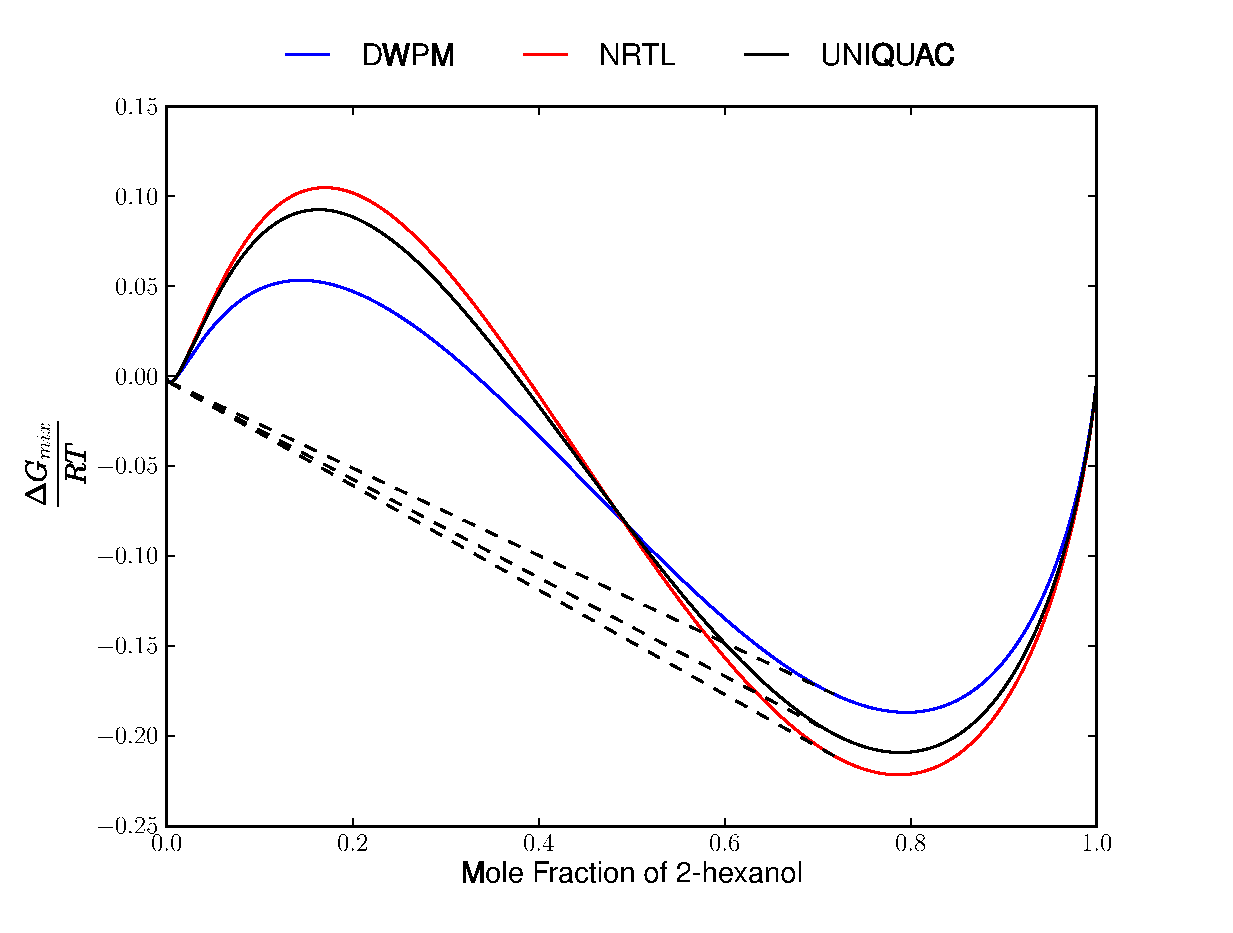
\includegraphics[width = \textwidth]{Results_Parts/BinaryParams/2-hexanol-water/AllModelsGibbsPlots/T_293.eps}
	\caption{293~$\mathrm{K}$} 
\end{subfigure}%
~%
\begin{subfigure}[h]{0.5\textwidth}
	\centering
	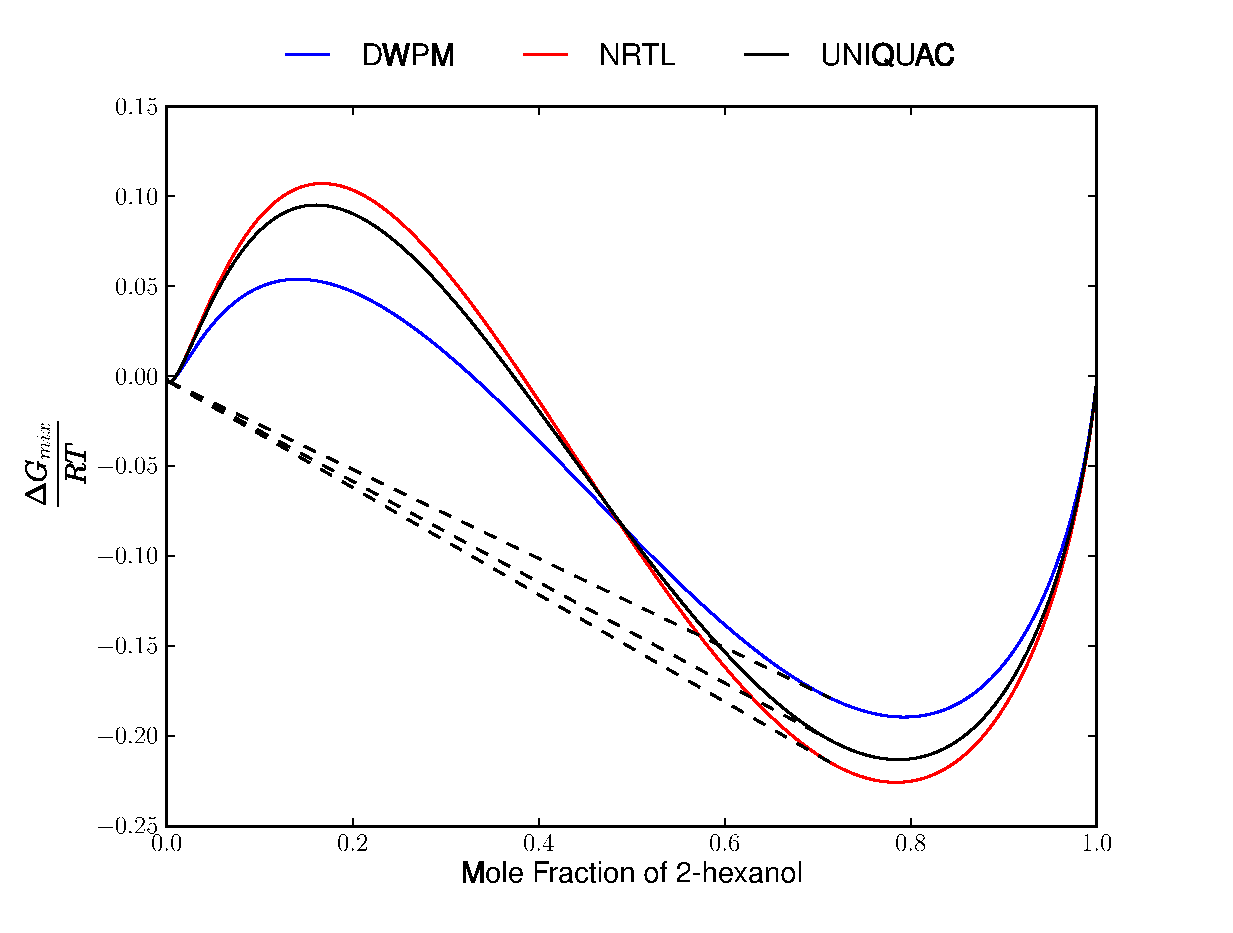
\includegraphics[width = \textwidth]{Results_Parts/BinaryParams/2-hexanol-water/AllModelsGibbsPlots/T_298.eps}
	\caption{298~$\mathrm{K}$}
\end{subfigure}%
\\%
\begin{subfigure}[h]{0.5\textwidth}
	\centering
	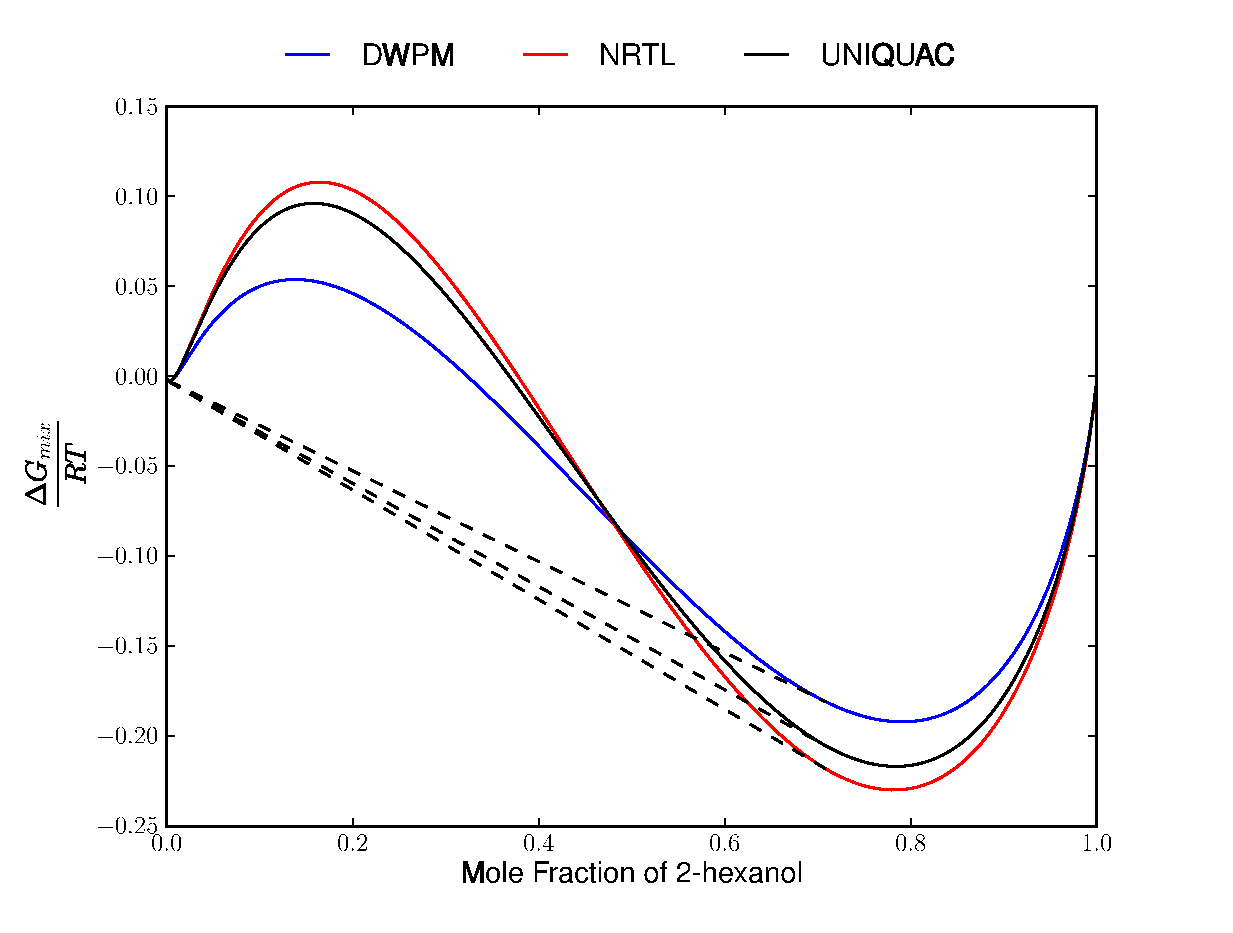
\includegraphics[width = \textwidth]{Results_Parts/BinaryParams/2-hexanol-water/AllModelsGibbsPlots/T_303.eps}
	\caption{303~$\mathrm{K}$} 
\end{subfigure}%
\caption{Calculated liquid-liquid equilibrium for 2-Hexanol and Water}
\end{figure}
\clearpage
%%------------------------------------------------------------------------------------------------------------------------------------------------%%
\subsection{13-Dimethyl Benzene and Water}
\vspace*{\fill}
\begin{figure}[hp]
\begin{subfigure}[h]{0.5\textwidth}
	\centering
	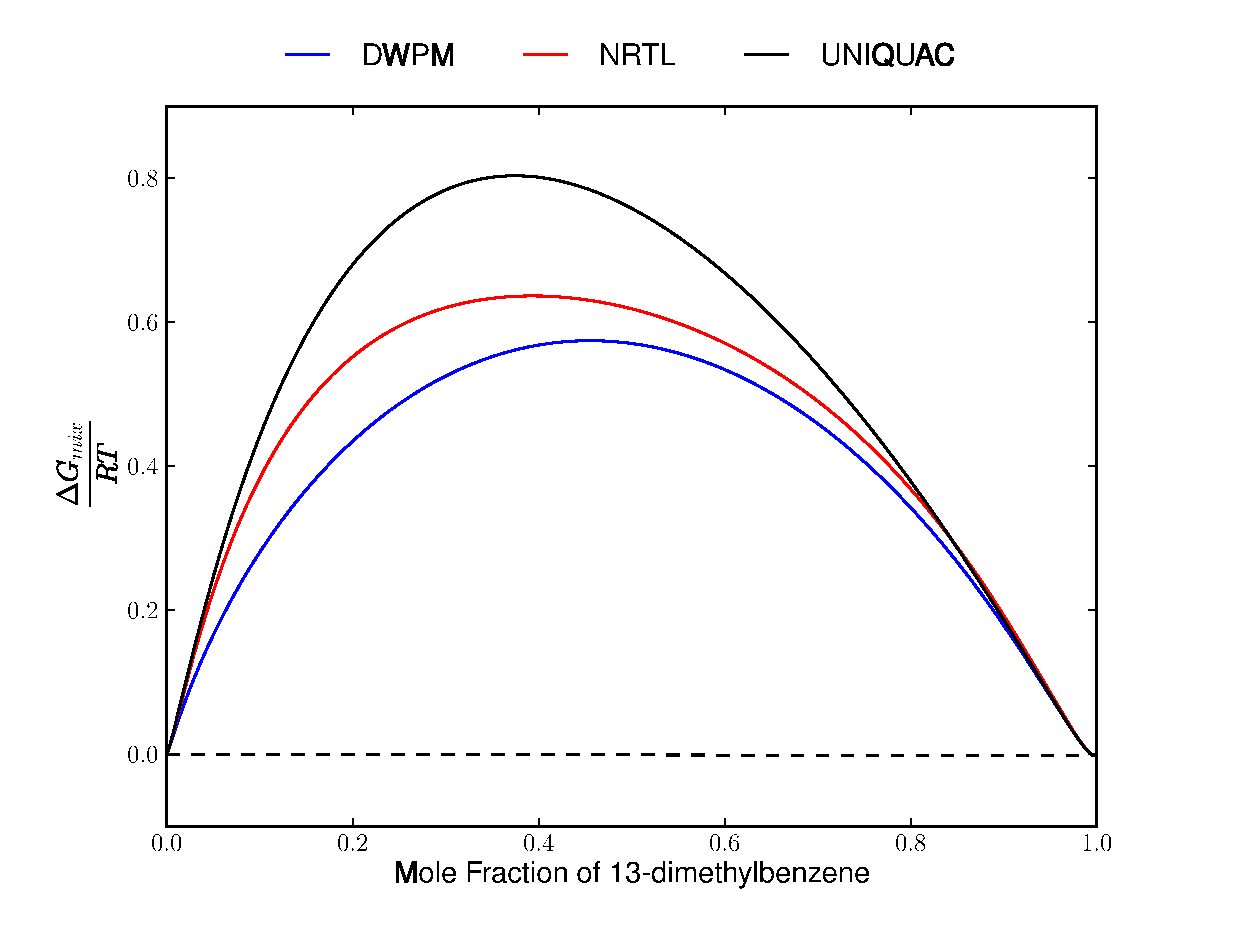
\includegraphics[width = \textwidth]{Results_Parts/BinaryParams/13-dimethylbenzene-water/AllModelsGibbsPlots/T_292.85.eps}
	\caption{292.85~$\mathrm{K}$} 
\end{subfigure}%
~%
\begin{subfigure}[h]{0.5\textwidth}
	\centering
	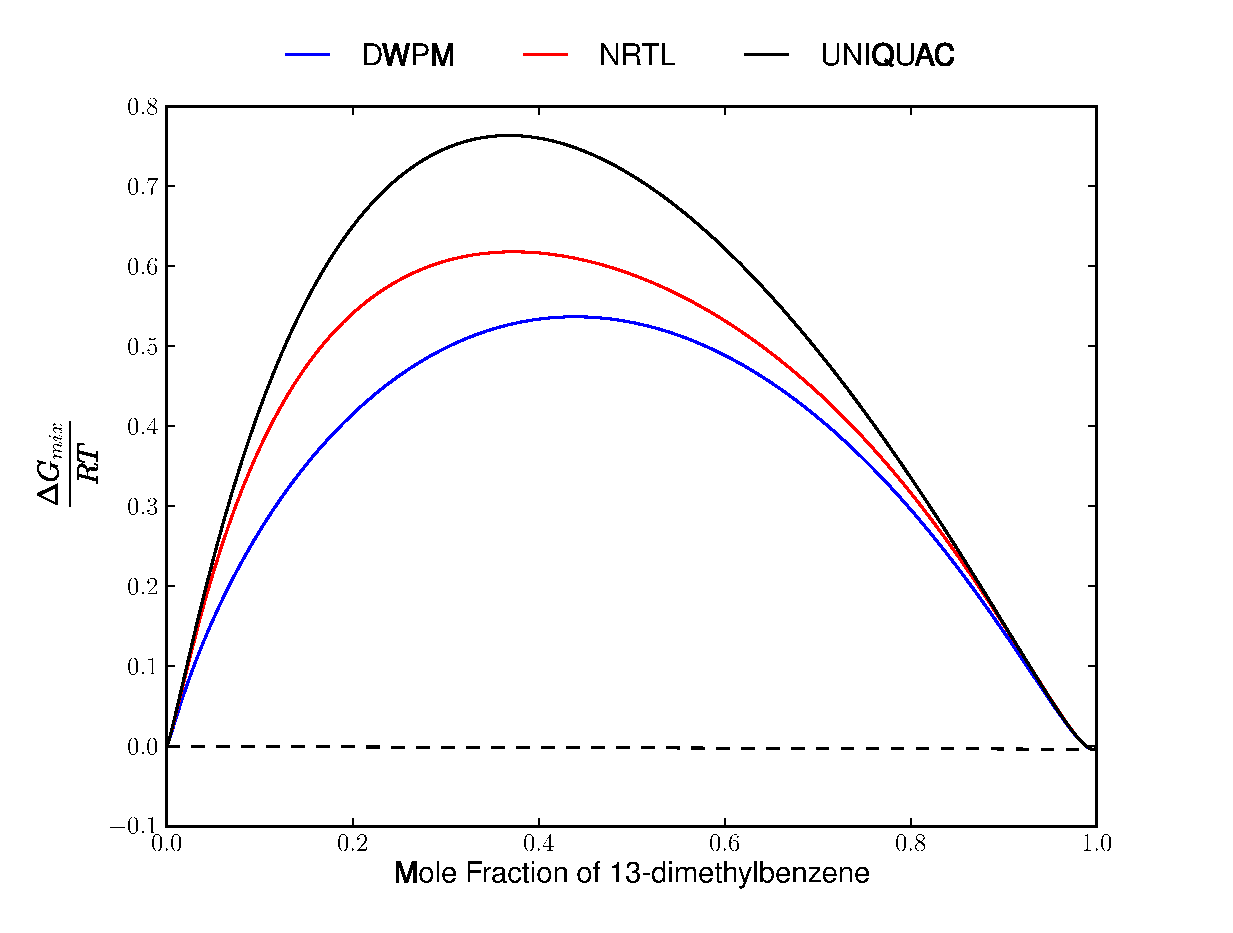
\includegraphics[width = \textwidth]{Results_Parts/BinaryParams/13-dimethylbenzene-water/AllModelsGibbsPlots/T_312.85.eps}
	\caption{312.85~$\mathrm{K}$} 
\end{subfigure}%
\\%
\begin{subfigure}[h]{0.5\textwidth}
\centering
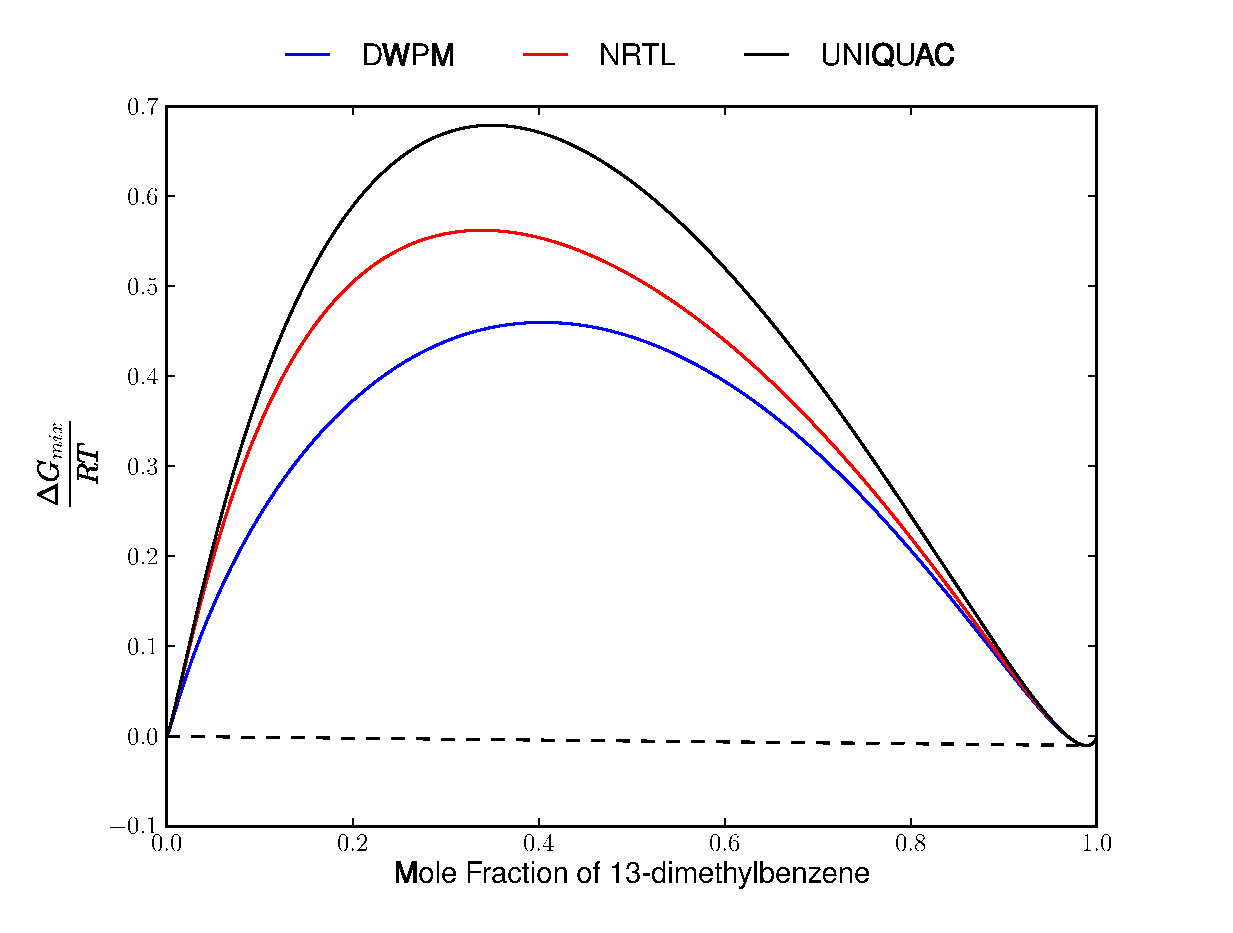
\includegraphics[width = \textwidth]{Results_Parts/BinaryParams/13-dimethylbenzene-water/AllModelsGibbsPlots/T_342.85.eps}
\caption{342.85~$\mathrm{K}$} 
\end{subfigure}%
\caption{Calculated liquid-liquid equilibrium for 13-Dimethyl Benzene and Water}
\end{figure}
\vspace*{\fill}
\clearpage
%%-------------------------------------------------------------------------------------------------------------------------------------------------%%
\subsection{Aniline and Water}
\vspace*{\fill}
\begin{figure}[hp]
\begin{subfigure}[h]{0.5\textwidth}
	\centering
	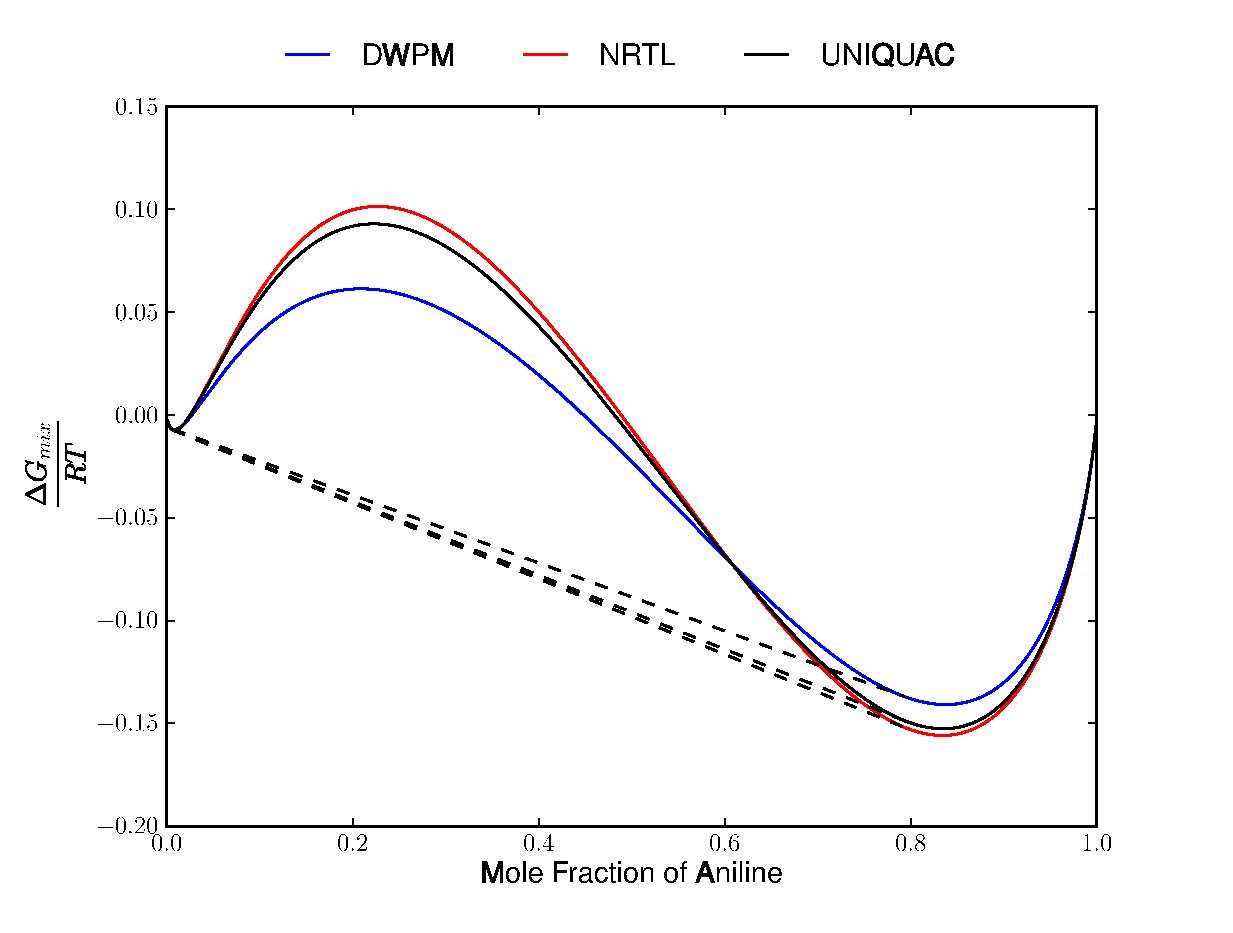
\includegraphics[width = \textwidth]{Results_Parts/BinaryParams/aniline-water/AllModelsGibbsPlots/T_281.6.eps}
	\caption{281.6~$\mathrm{K}$} 
\end{subfigure}%
~%
\begin{subfigure}[h]{0.5\textwidth}
	\centering
	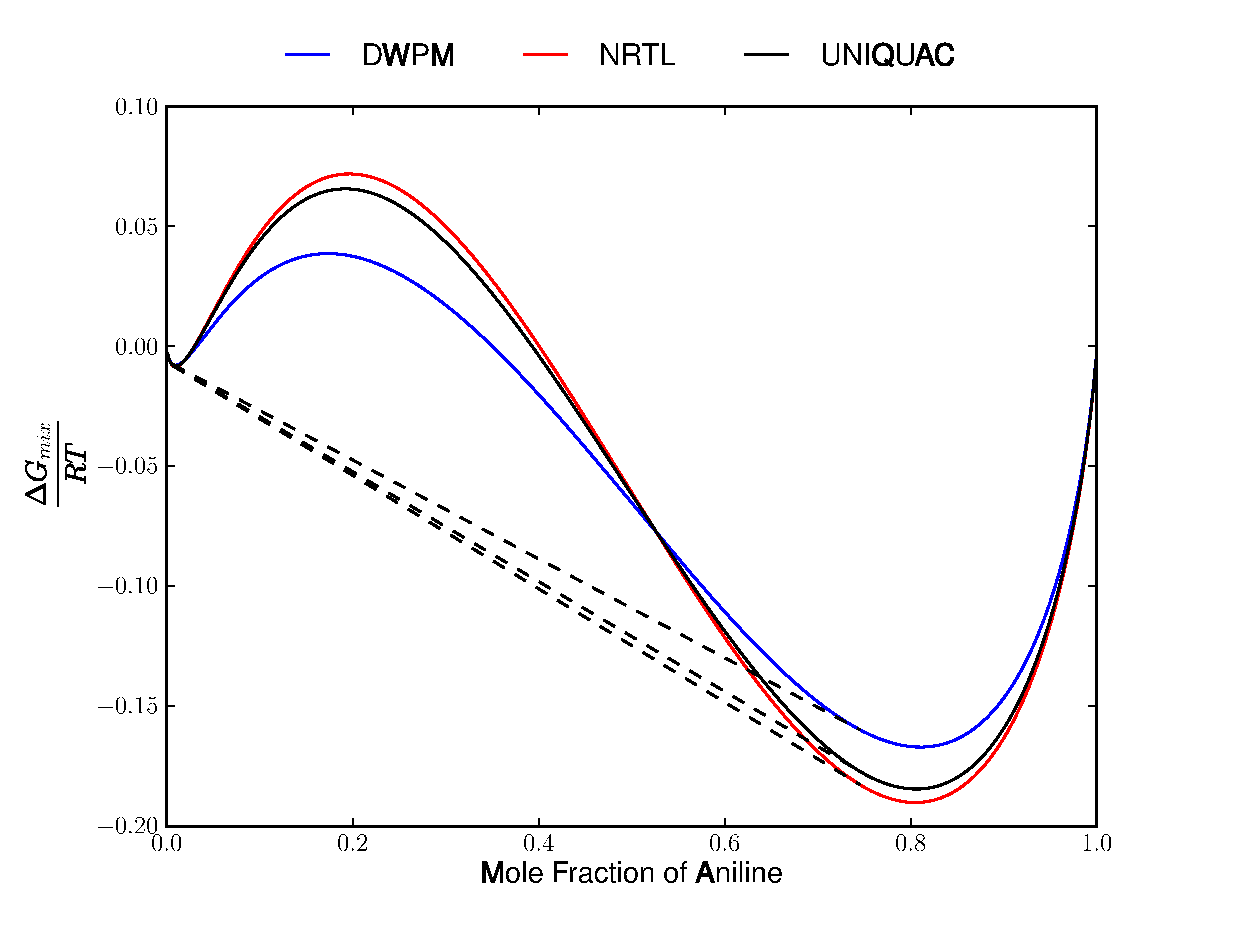
\includegraphics[width = \textwidth]{Results_Parts/BinaryParams/aniline-water/AllModelsGibbsPlots/T_298.4.eps}
	\caption{298.4~$\mathrm{K}$} 
\end{subfigure}%
\\%
\begin{subfigure}[h]{0.5\textwidth}
	\centering
	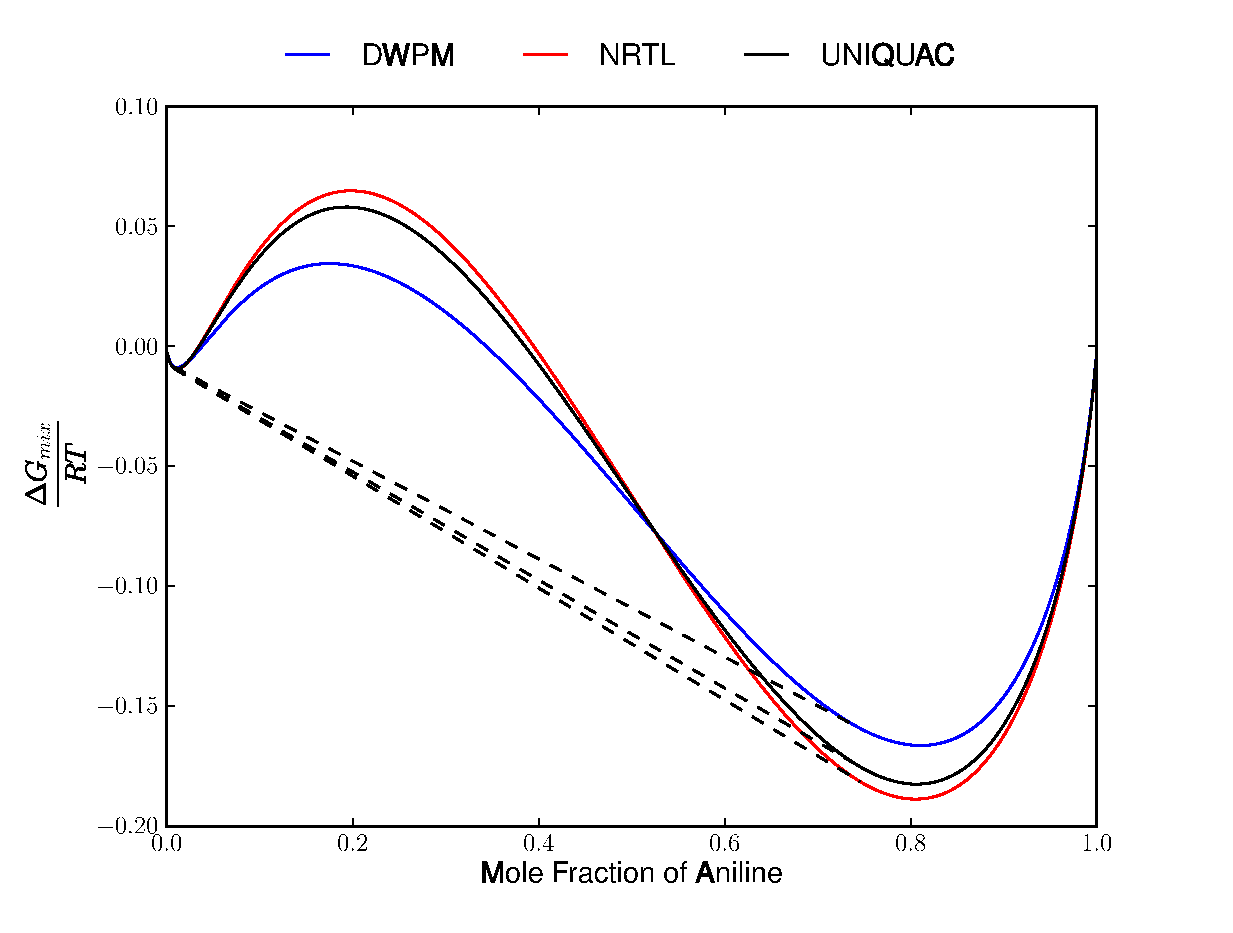
\includegraphics[width = \textwidth]{Results_Parts/BinaryParams/aniline-water/AllModelsGibbsPlots/T_321.0.eps}
	\caption{321.0~$\mathrm{K}$} 
\end{subfigure}%
~%
\begin{subfigure}[h]{0.5\textwidth}
	\centering
	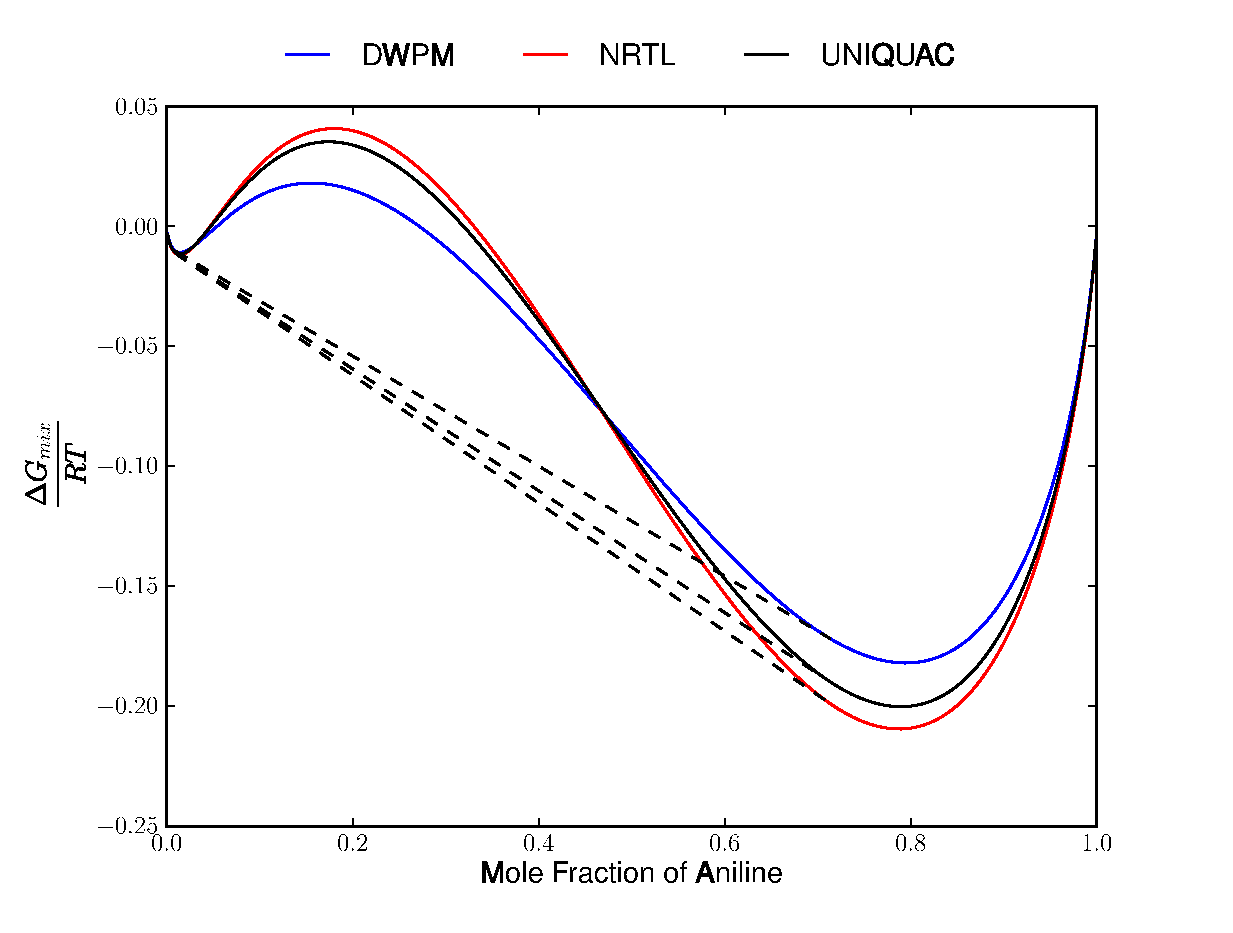
\includegraphics[width = \textwidth]{Results_Parts/BinaryParams/aniline-water/AllModelsGibbsPlots/T_339.3.eps}
	\caption{339.3~$\mathrm{K}$} 
\end{subfigure}%
\caption{Calculated liquid-liquid equilibrium for Aniline and Water}
\end{figure}
\vspace*{\fill}
\clearpage
\begin{figure}[hpt]
\ContinuedFloat 
\begin{subfigure}[h]{0.5\textwidth}
\centering
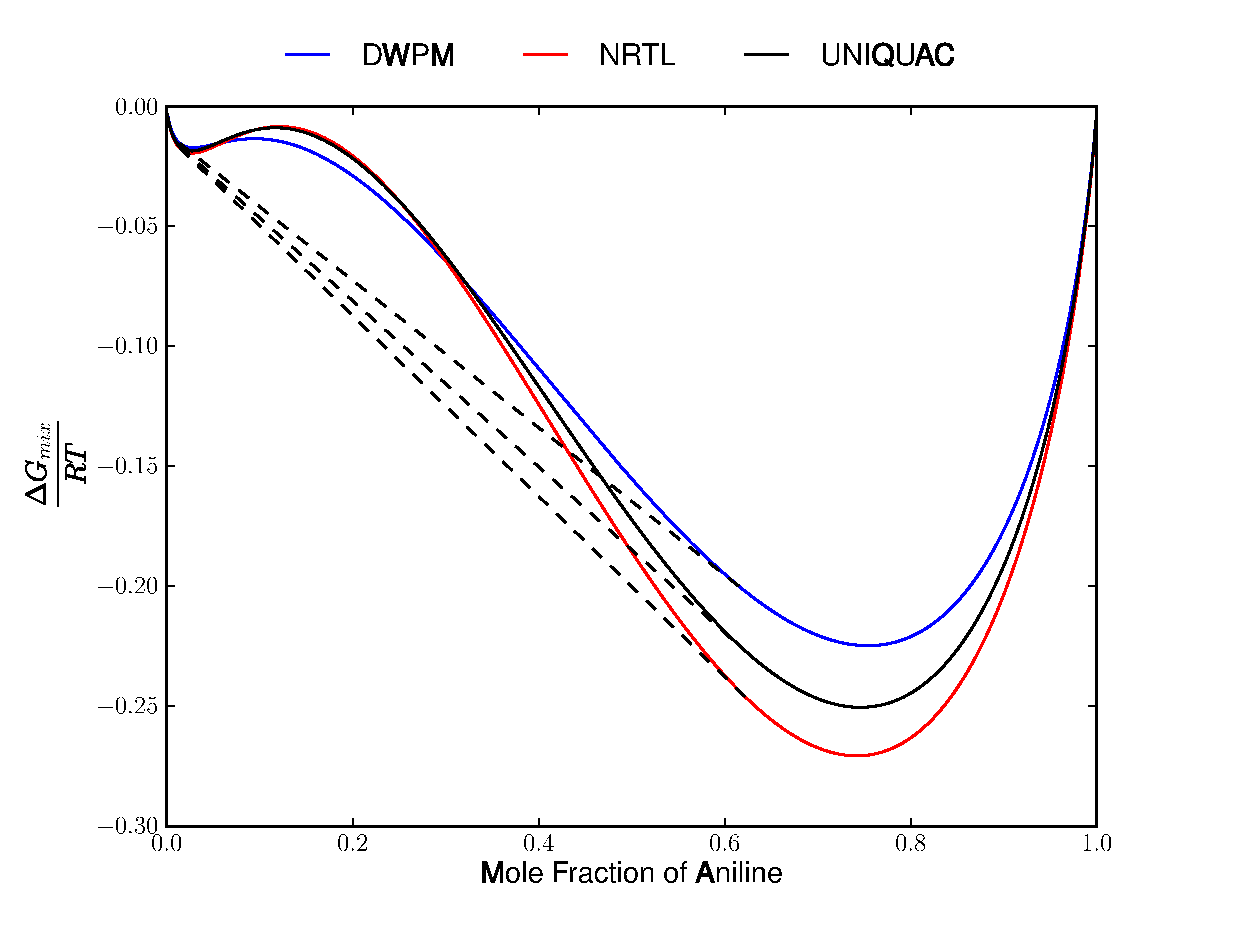
\includegraphics[width = \textwidth]{Results_Parts/BinaryParams/aniline-water/AllModelsGibbsPlots/T_369.7.eps}
\caption{369.7~$\mathrm{K}$}
\end{subfigure}%
\caption[]{Calculated liquid-liquid equilibrium for Aniline and Water}
\end{figure}
\clearpage

%%-------------------------------------------------------------------------------------------------------------------------------------------------%%

\subsection{Diethylene Glycol and 12-Dimethyl Benzene}
\vspace*{\fill}
\begin{figure}[hp]
\begin{subfigure}[h]{0.5\textwidth}
	\centering
	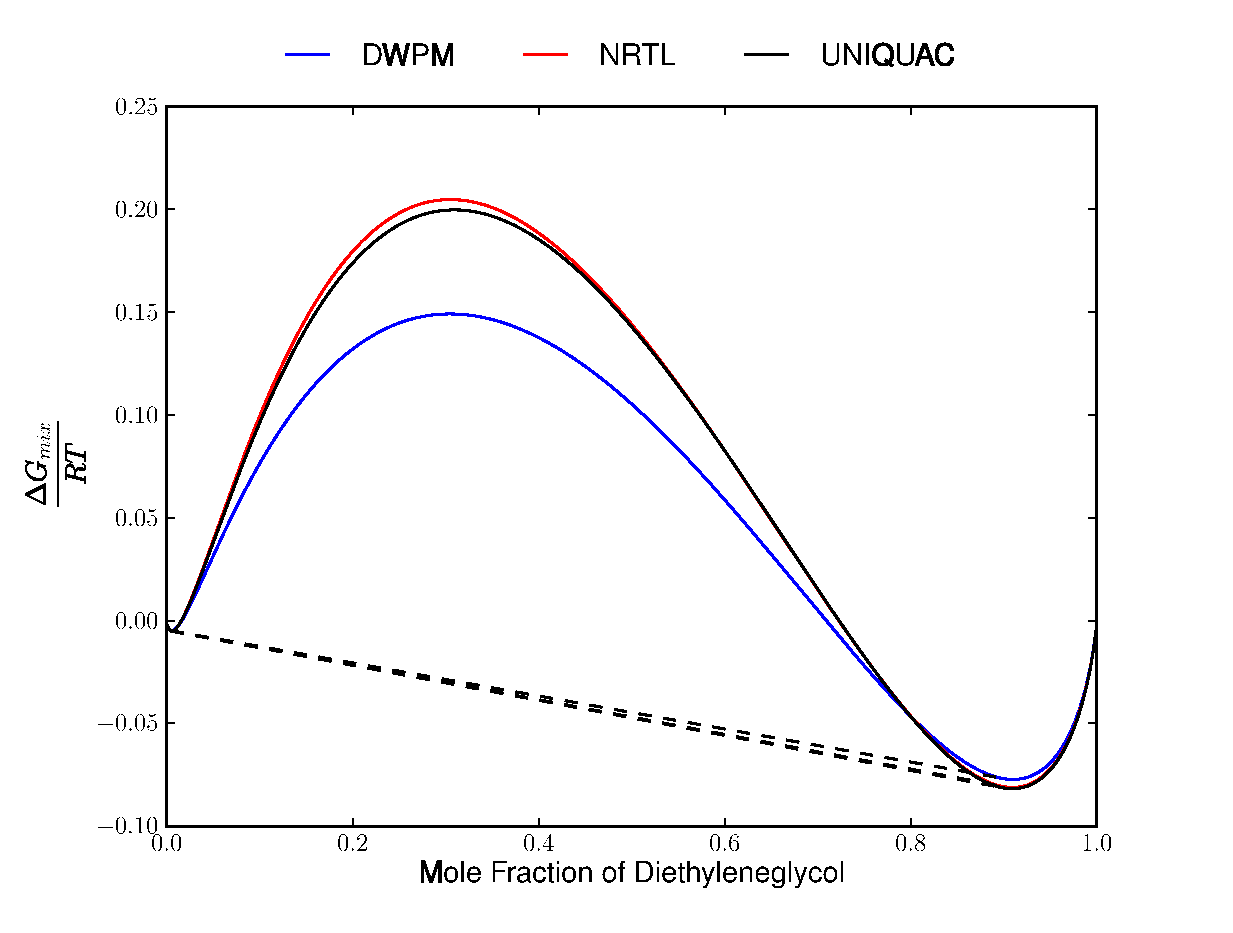
\includegraphics[width = \textwidth]{Results_Parts/BinaryParams/diethyleneglycol-12-dimethylbenzene/AllModelsGibbsPlots/T_313.3.eps}
	\caption{313.3~$\mathrm{K}$} 
\end{subfigure}%
~%
\begin{subfigure}[h]{0.5\textwidth}
	\centering
	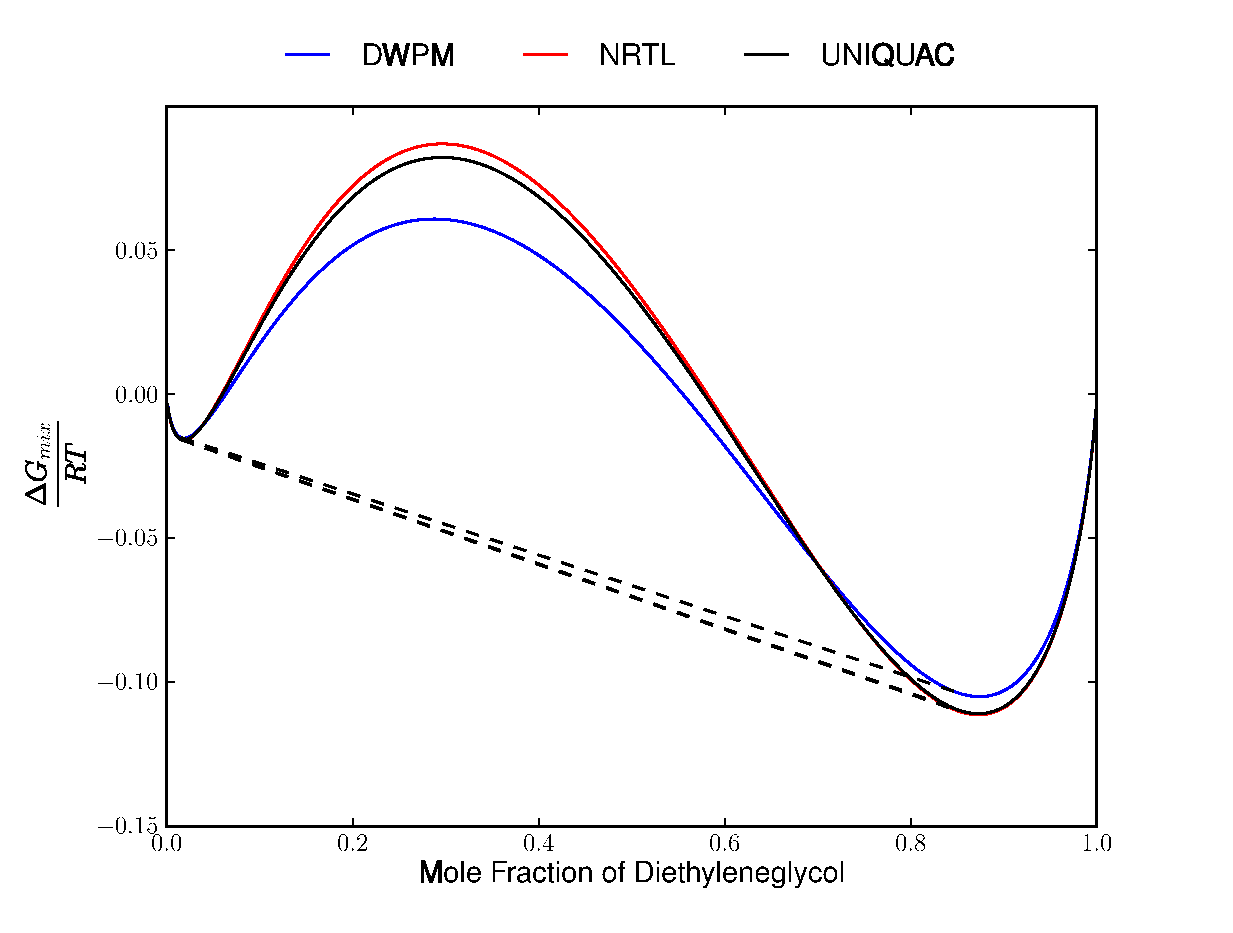
\includegraphics[width = \textwidth]{Results_Parts/BinaryParams/diethyleneglycol-12-dimethylbenzene/AllModelsGibbsPlots/T_332.8.eps}
	\caption{332.8~$\mathrm{K}$} 
\end{subfigure}%
\\%
\begin{subfigure}[h]{0.5\textwidth}
	\centering
	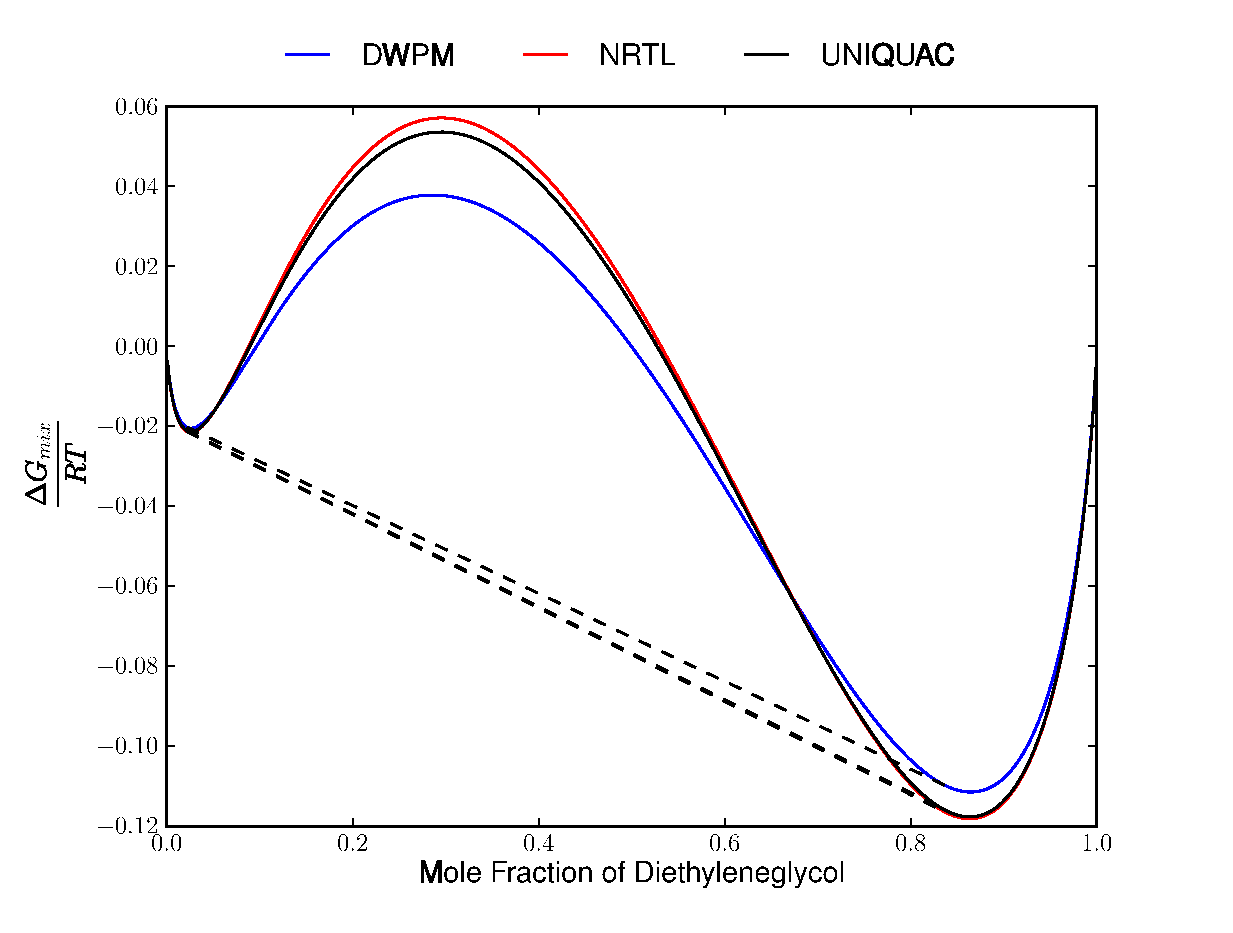
\includegraphics[width = \textwidth]{Results_Parts/BinaryParams/diethyleneglycol-12-dimethylbenzene/AllModelsGibbsPlots/T_353.8.eps}
	\caption{383.8~$\mathrm{K}$} 
\end{subfigure}%
~%
\begin{subfigure}[h]{0.5\textwidth}
	\centering
	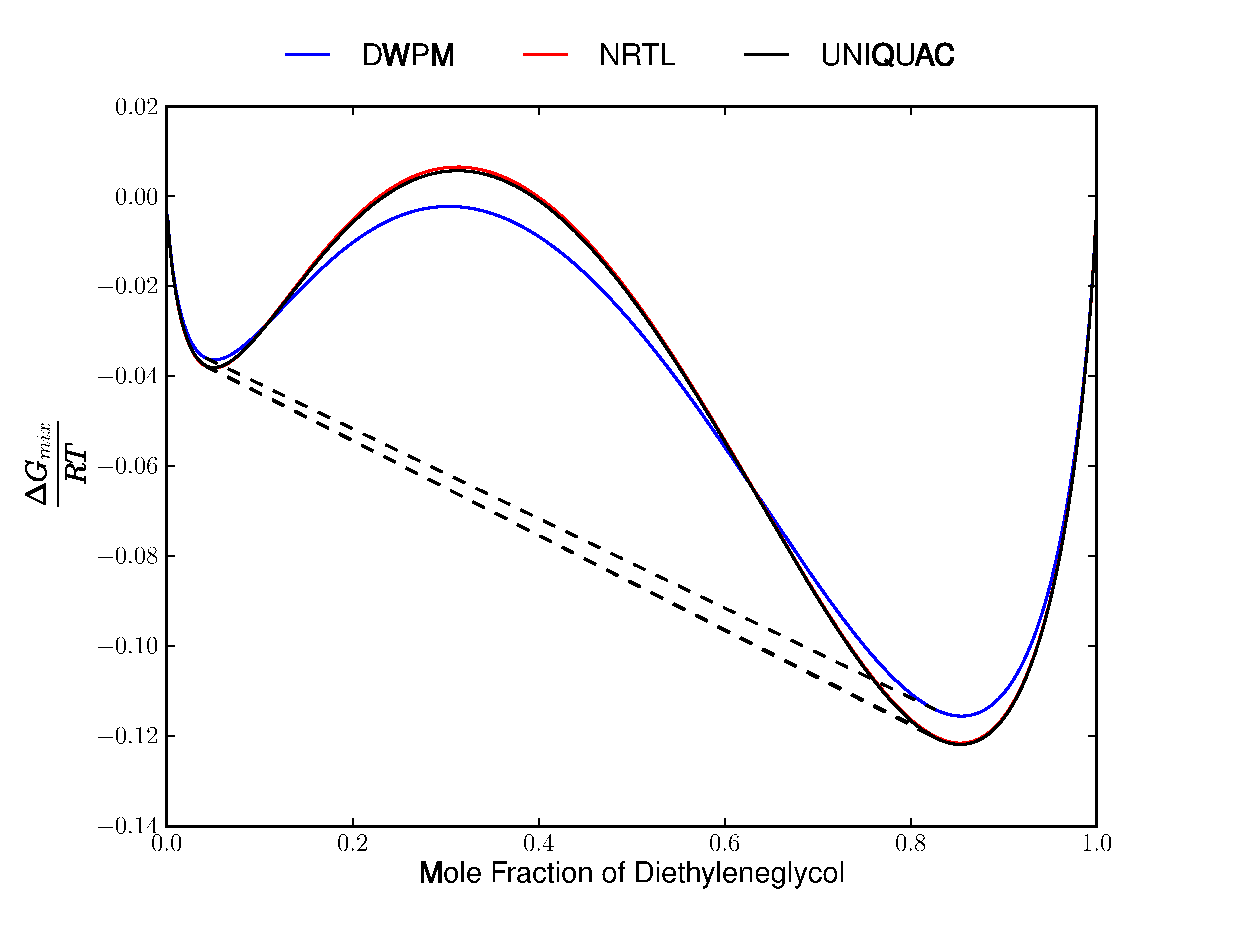
\includegraphics[width = \textwidth]{Results_Parts/BinaryParams/diethyleneglycol-12-dimethylbenzene/AllModelsGibbsPlots/T_363.0.eps}
	\caption{363.0~$\mathrm{K}$} 
\end{subfigure}%
\caption{Calculated liquid-liquid equilibrium for Diethylene Glycol and 12-Dimethyl Benzene}
\end{figure}
\vspace*{\fill}
\clearpage
\begin{figure}[hpt]
\ContinuedFloat 
\begin{subfigure}[h]{0.5\textwidth}
	\centering
	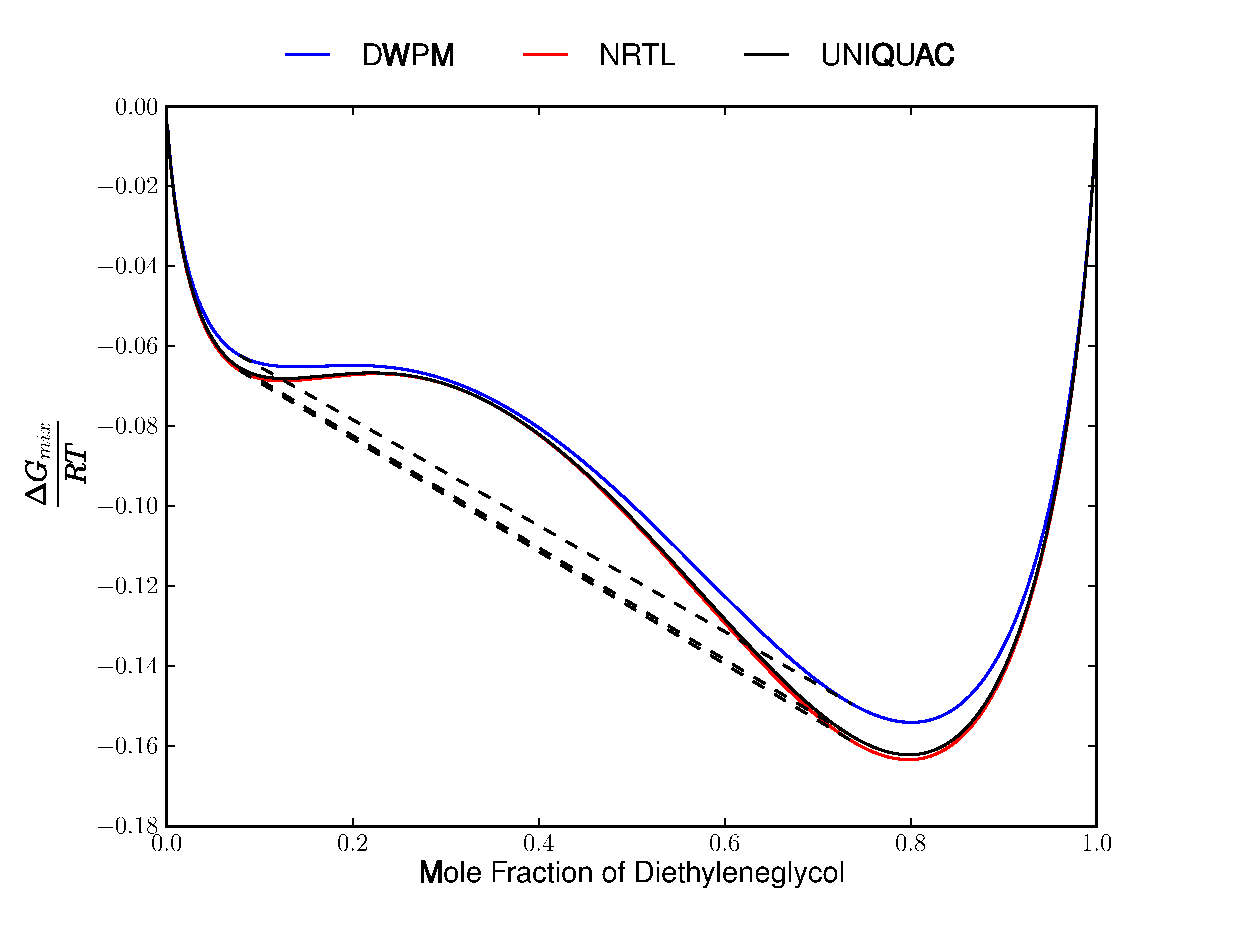
\includegraphics[width = \textwidth]{Results_Parts/BinaryParams/diethyleneglycol-12-dimethylbenzene/AllModelsGibbsPlots/T_393.0.eps}
	\caption{393.0~$\mathrm{K}$} 
\end{subfigure}
\caption[]{Calculated liquid-liquid equilibrium for Diethylene Glycol and 12-Dimethyl Benzene}
\end{figure}
\clearpage

%%------------------------------------------------------------------------------------------------------------------------------------------------%%

\subsection{Dipropyl Ether and Water}
\vspace*{\fill}
\begin{figure}[hp]
\begin{subfigure}[h]{0.5\textwidth}
	\centering
	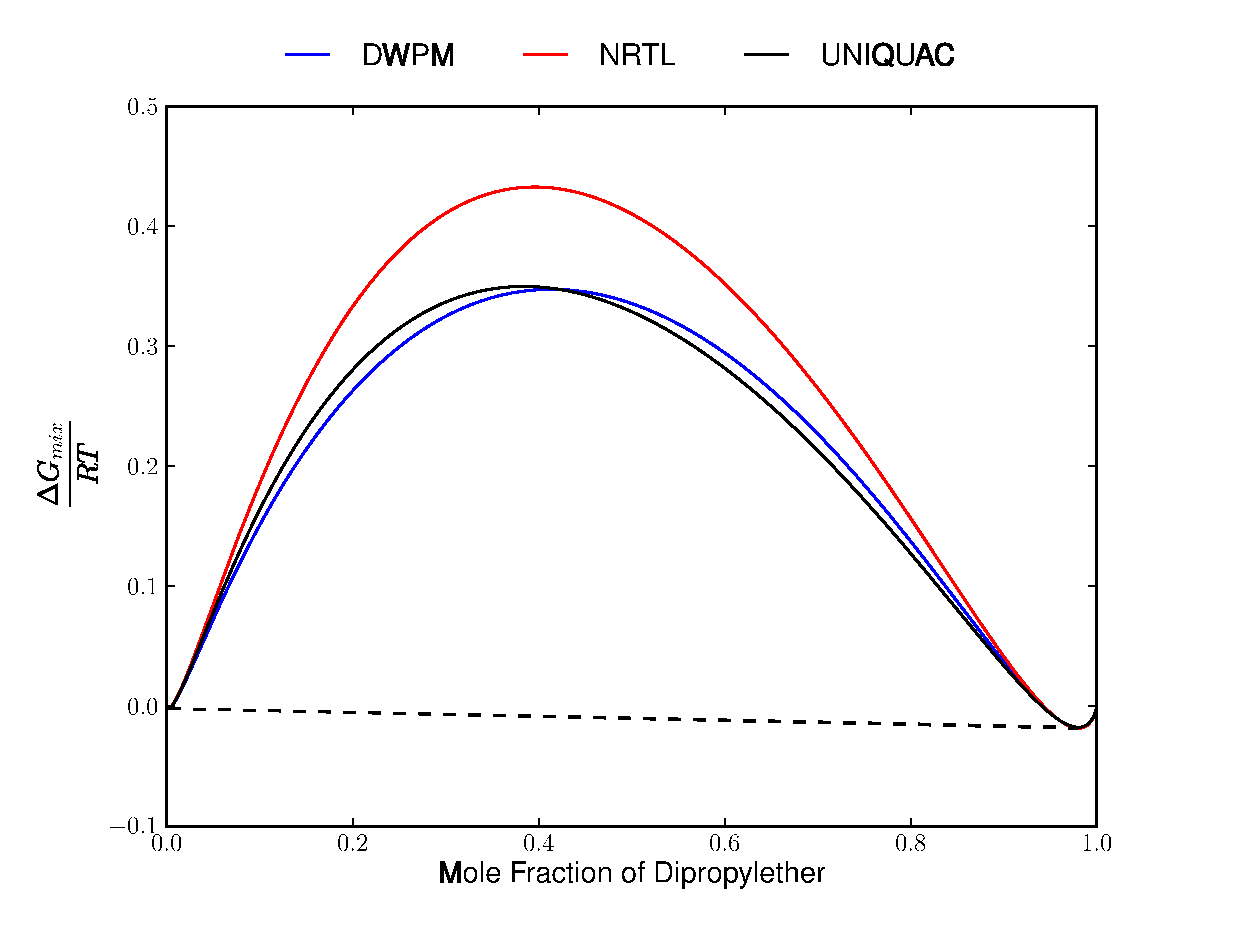
\includegraphics[width = \textwidth]{Results_Parts/BinaryParams/dipropylether-water/AllModelsGibbsPlots/T_273.eps}
	\caption{273.0~$\mathrm{K}$} 
\end{subfigure}%
~%
\begin{subfigure}[h]{0.5\textwidth}
	\centering
	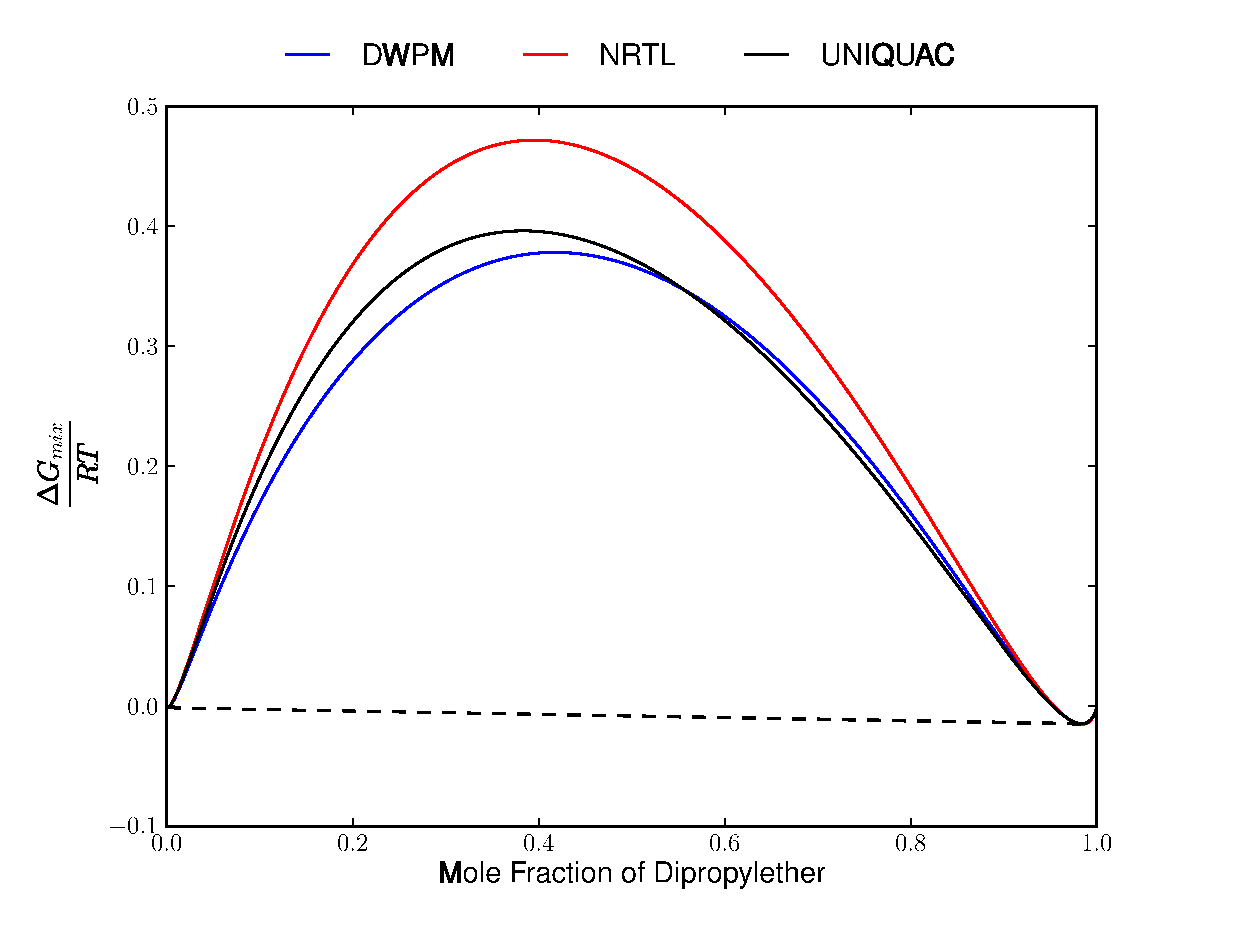
\includegraphics[width = \textwidth]{Results_Parts/BinaryParams/dipropylether-water/AllModelsGibbsPlots/T_283.eps}
	\caption{283.0~$\mathrm{K}$} 
\end{subfigure}%
\\%
\begin{subfigure}[h]{0.5\textwidth}
	\centering
	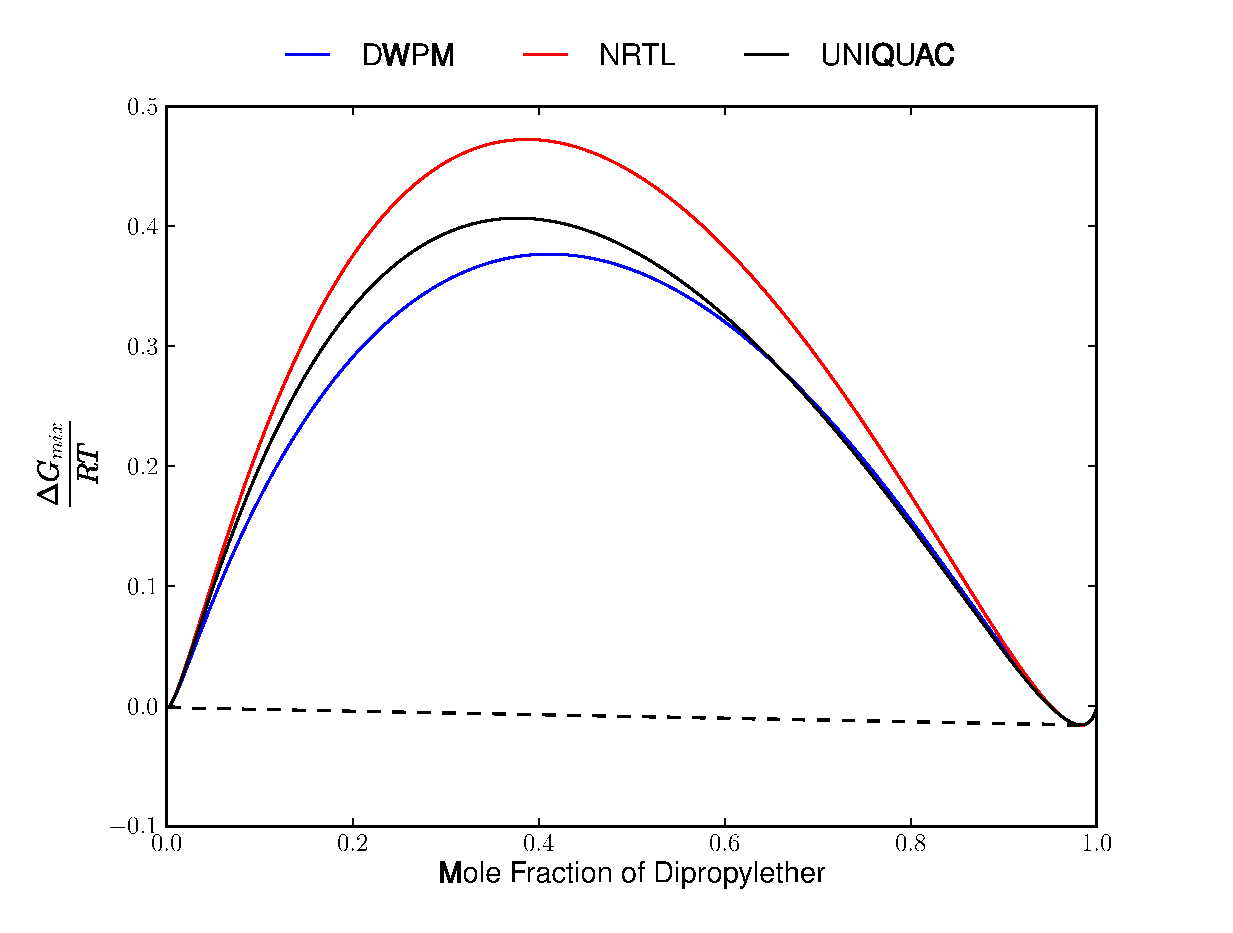
\includegraphics[width = \textwidth]{Results_Parts/BinaryParams/dipropylether-water/AllModelsGibbsPlots/T_288.eps}
	\caption{288.0~$\mathrm{K}$} 
\end{subfigure}%
~%
\begin{subfigure}[h]{0.5\textwidth}
	\centering
	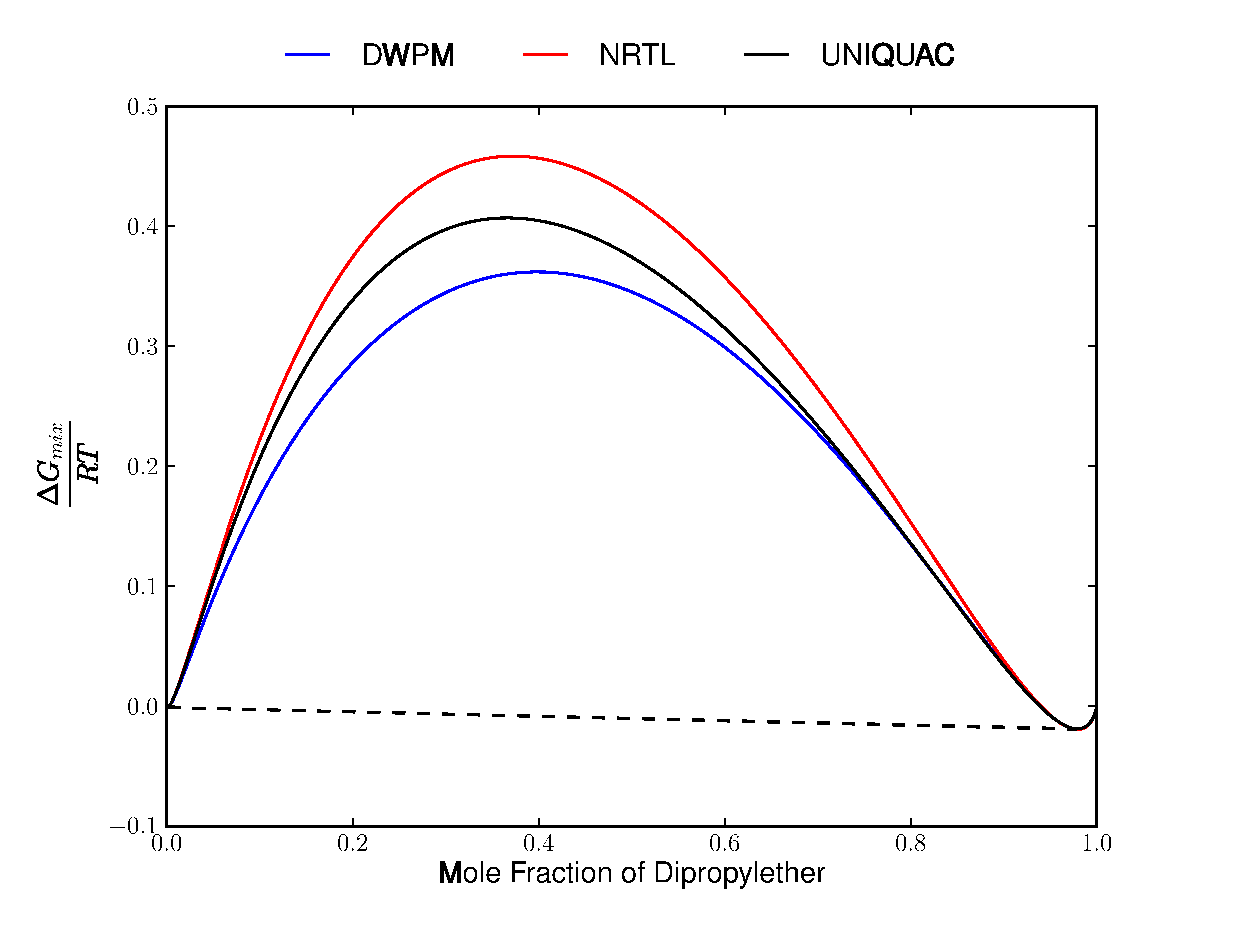
\includegraphics[width = \textwidth]{Results_Parts/BinaryParams/dipropylether-water/AllModelsGibbsPlots/T_293.eps}
	\caption{293.0~$\mathrm{K}$} 
\end{subfigure}%
\caption{Calculated liquid-liquid equilibrium for Dipropyl Ether and Water}
\end{figure}
\vspace*{\fill}
\clearpage
\begin{figure}[hpt]
\ContinuedFloat 
\begin{subfigure}[h]{0.5\textwidth}
	\centering
	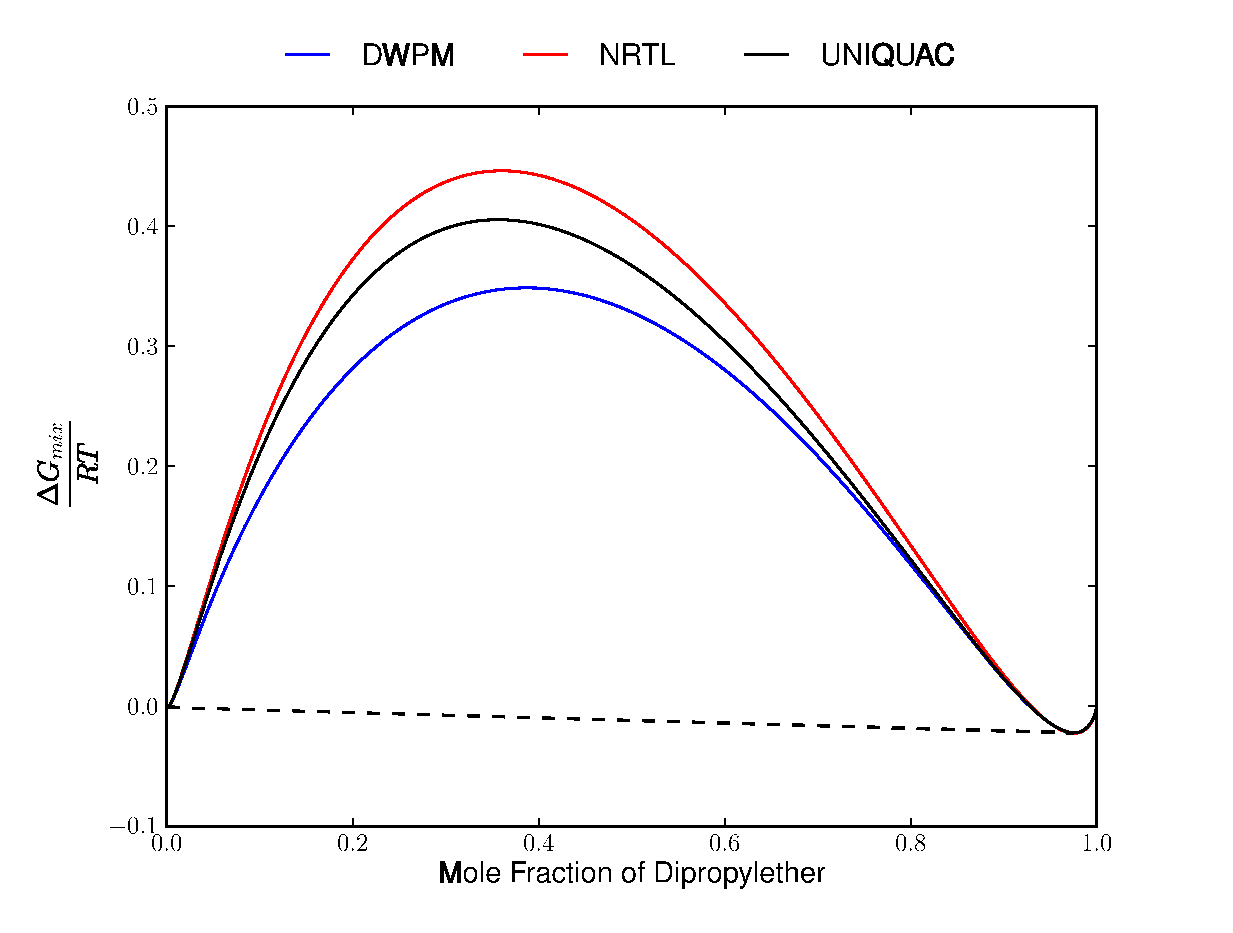
\includegraphics[width = \textwidth]{Results_Parts/BinaryParams/dipropylether-water/AllModelsGibbsPlots/T_298.eps}
	\caption{298.0~$\mathrm{K}$}
\end{subfigure}%
\caption[]{Calculated liquid-liquid equilibrium for Dipropyl Ether and Water}
\end{figure}
\clearpage

%%------------------------------------------------------------------------------------------------------------------------------------------------%%

\subsection{Ethyl Ester Acetic Acid and Water}
\vspace*{\fill}
\begin{figure}[hp]
\begin{subfigure}[h]{0.5\textwidth}
	\centering
	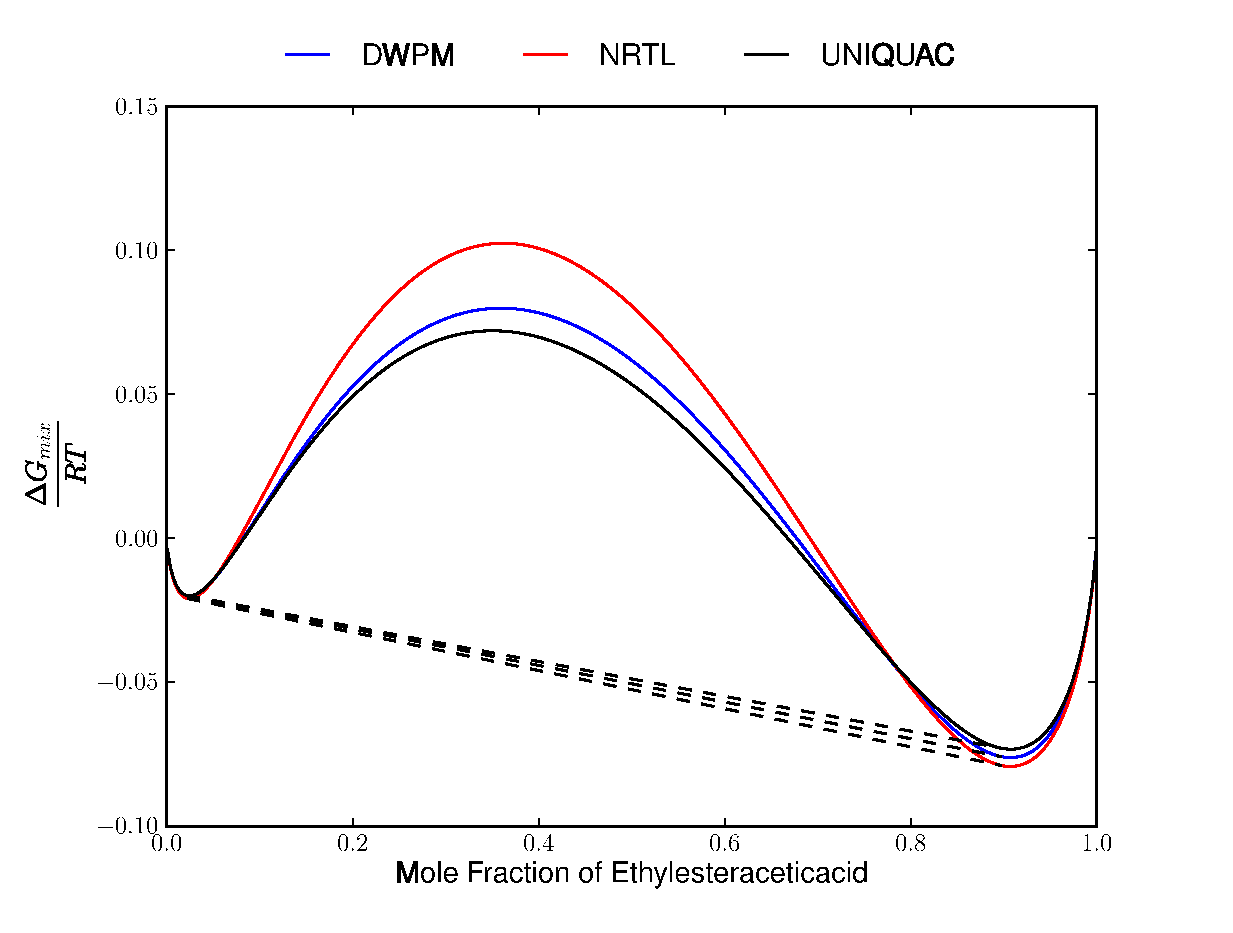
\includegraphics[width = \textwidth]{Results_Parts/BinaryParams/ethylesteraceticacid-water/AllModelsGibbsPlots/T_273.0.eps}
	\caption{273.0~$\mathrm{K}$} 
\end{subfigure}%
~%
\begin{subfigure}[h]{0.5\textwidth}
	\centering
	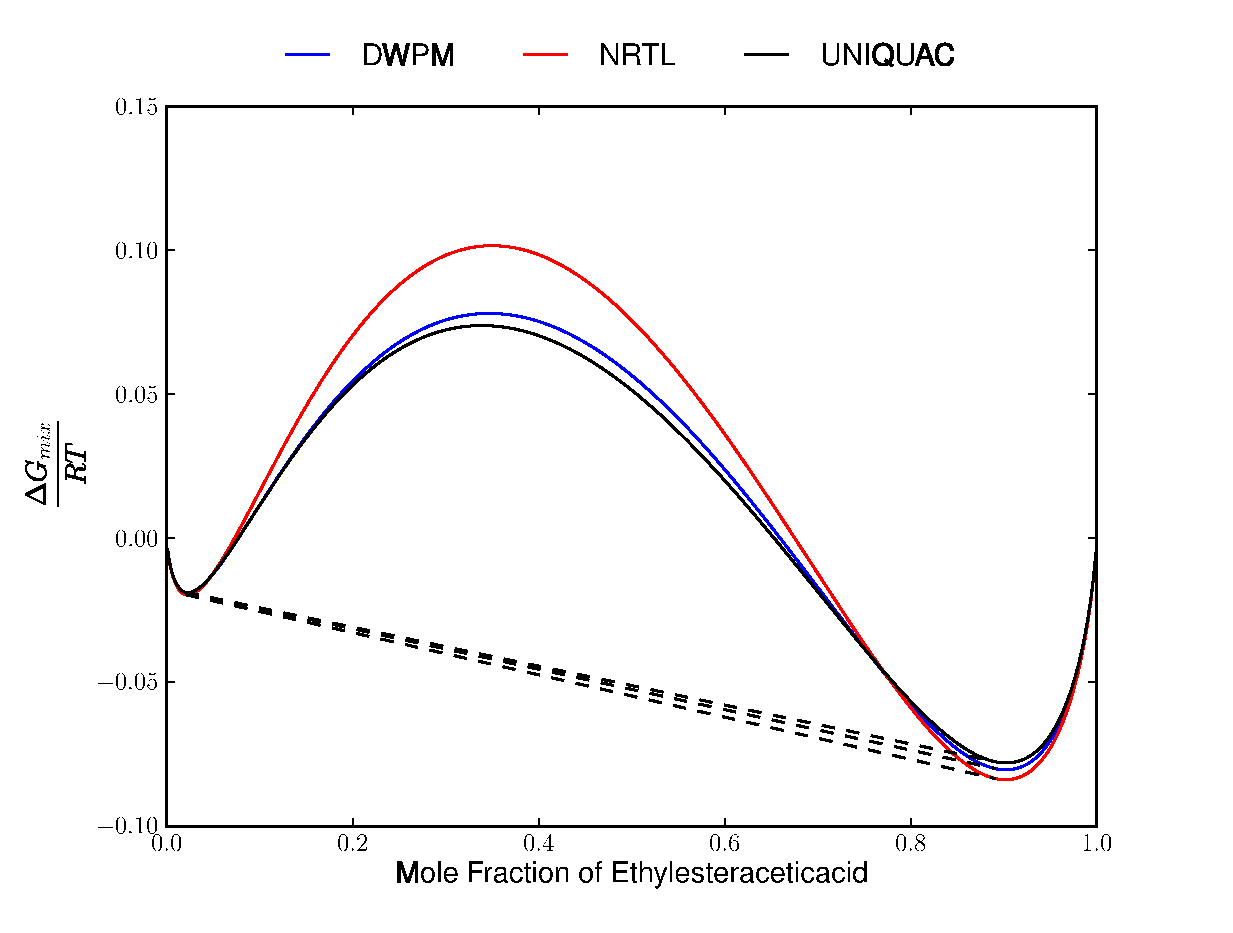
\includegraphics[width = \textwidth]{Results_Parts/BinaryParams/ethylesteraceticacid-water/AllModelsGibbsPlots/T_278.0.eps}
	\caption{278.0~$\mathrm{K}$} 
\end{subfigure}%
\\%
\begin{subfigure}[h]{0.5\textwidth}
	\centering
	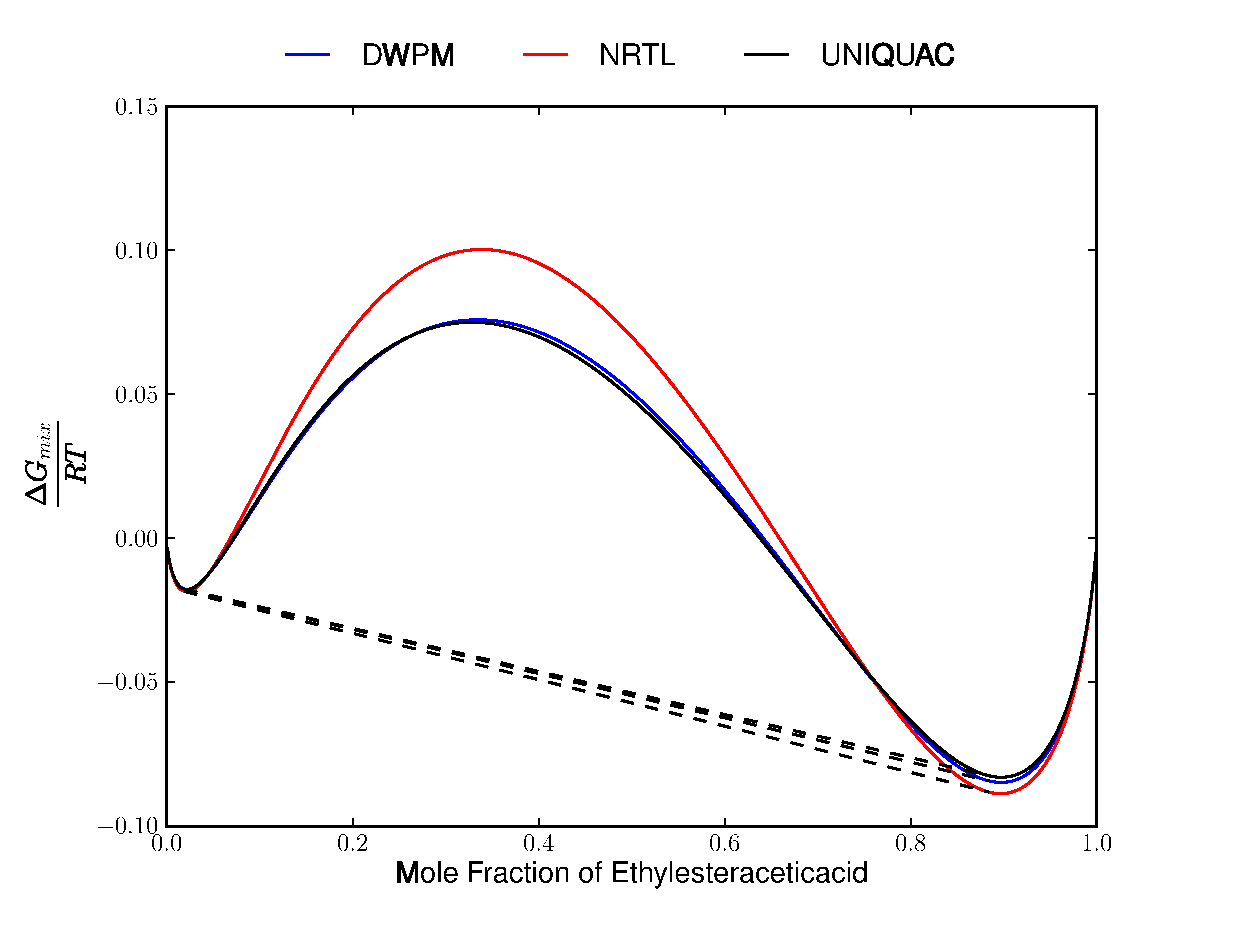
\includegraphics[width = \textwidth]{Results_Parts/BinaryParams/ethylesteraceticacid-water/AllModelsGibbsPlots/T_283.0.eps}
	\caption{283.0~$\mathrm{K}$}
\end{subfigure}%
~%
\begin{subfigure}[h]{0.5\textwidth}
	\centering
	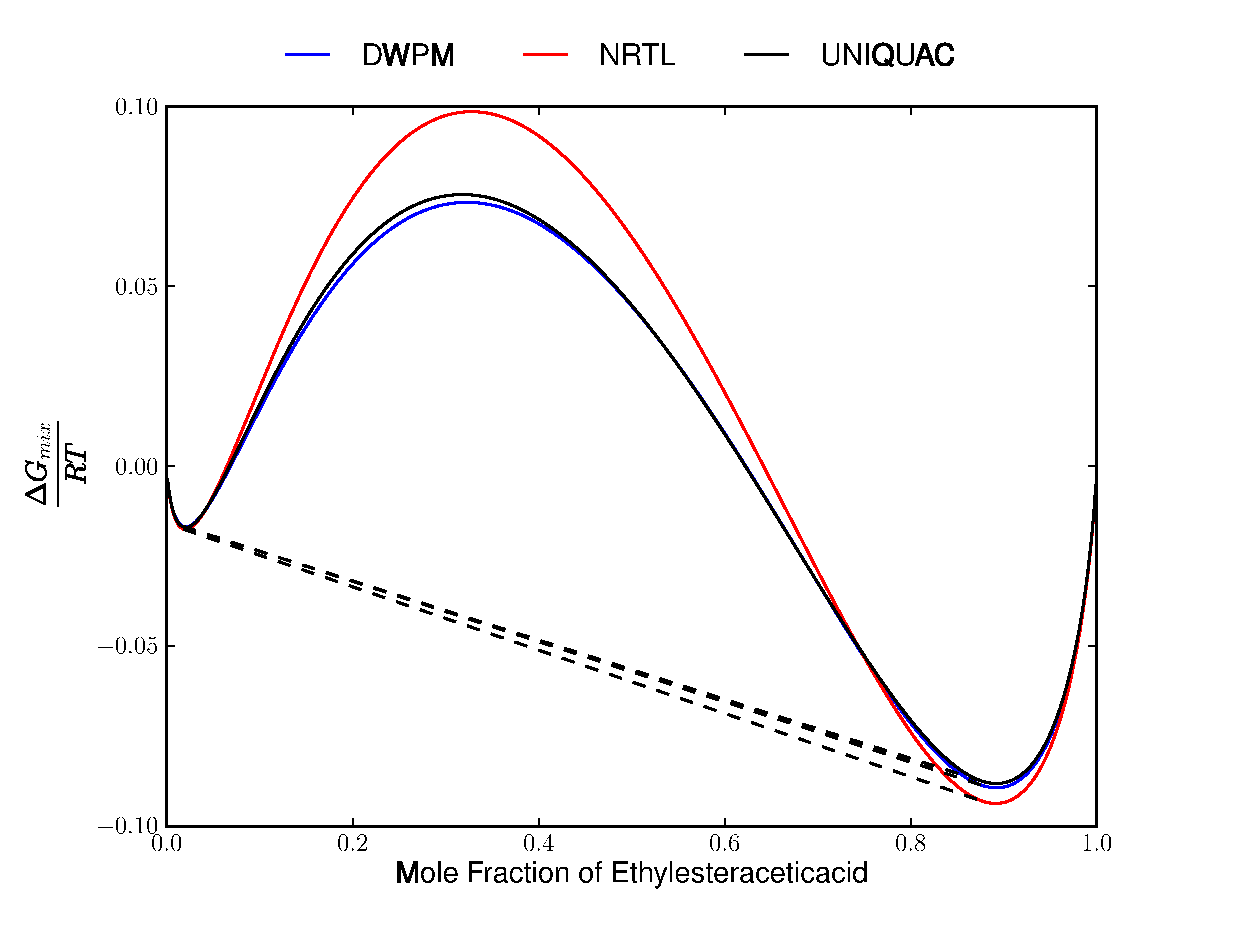
\includegraphics[width = \textwidth]{Results_Parts/BinaryParams/ethylesteraceticacid-water/AllModelsGibbsPlots/T_288.0.eps}
	\caption{288.0~$\mathrm{K}$}
\end{subfigure}%
\caption{Calculated liquid-liquid equilibrium for Ethyl Ester Acetic Acid and Water}
\end{figure}
\vspace*{\fill}
\clearpage
\vspace*{\fill}
\begin{figure}[hp]
\ContinuedFloat 
\begin{subfigure}[h]{0.5\textwidth}
	\centering
	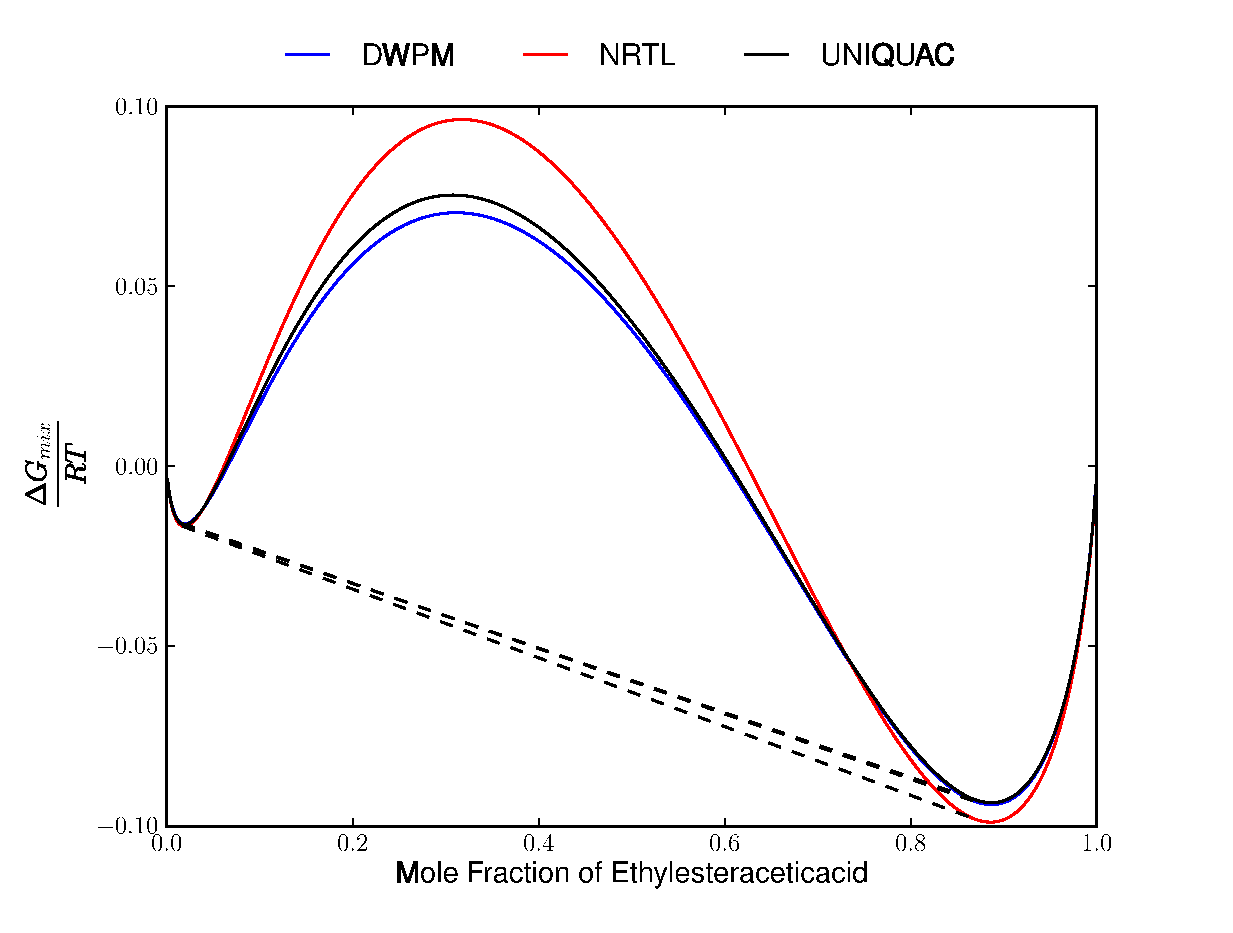
\includegraphics[width = \textwidth]{Results_Parts/BinaryParams/ethylesteraceticacid-water/AllModelsGibbsPlots/T_293.0.eps}
	\caption{293.0~$\mathrm{K}$}
\end{subfigure}%
~%
\begin{subfigure}[h]{0.5\textwidth}
	\centering
	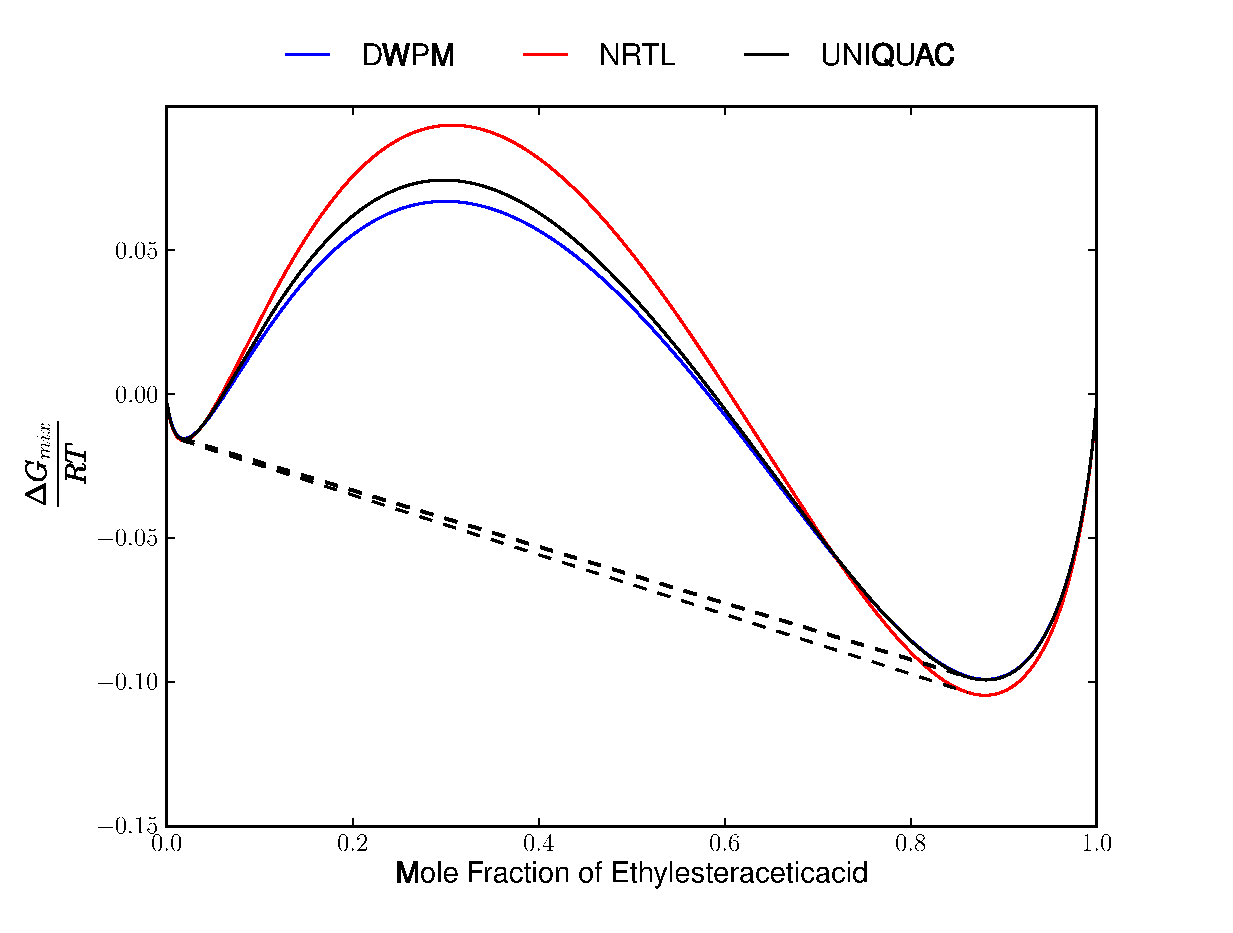
\includegraphics[width = \textwidth]{Results_Parts/BinaryParams/ethylesteraceticacid-water/AllModelsGibbsPlots/T_298.0.eps}
	\caption{298.0~$\mathrm{K}$}
\end{subfigure}%
\\%
\begin{subfigure}[h]{0.5\textwidth}
	\centering
	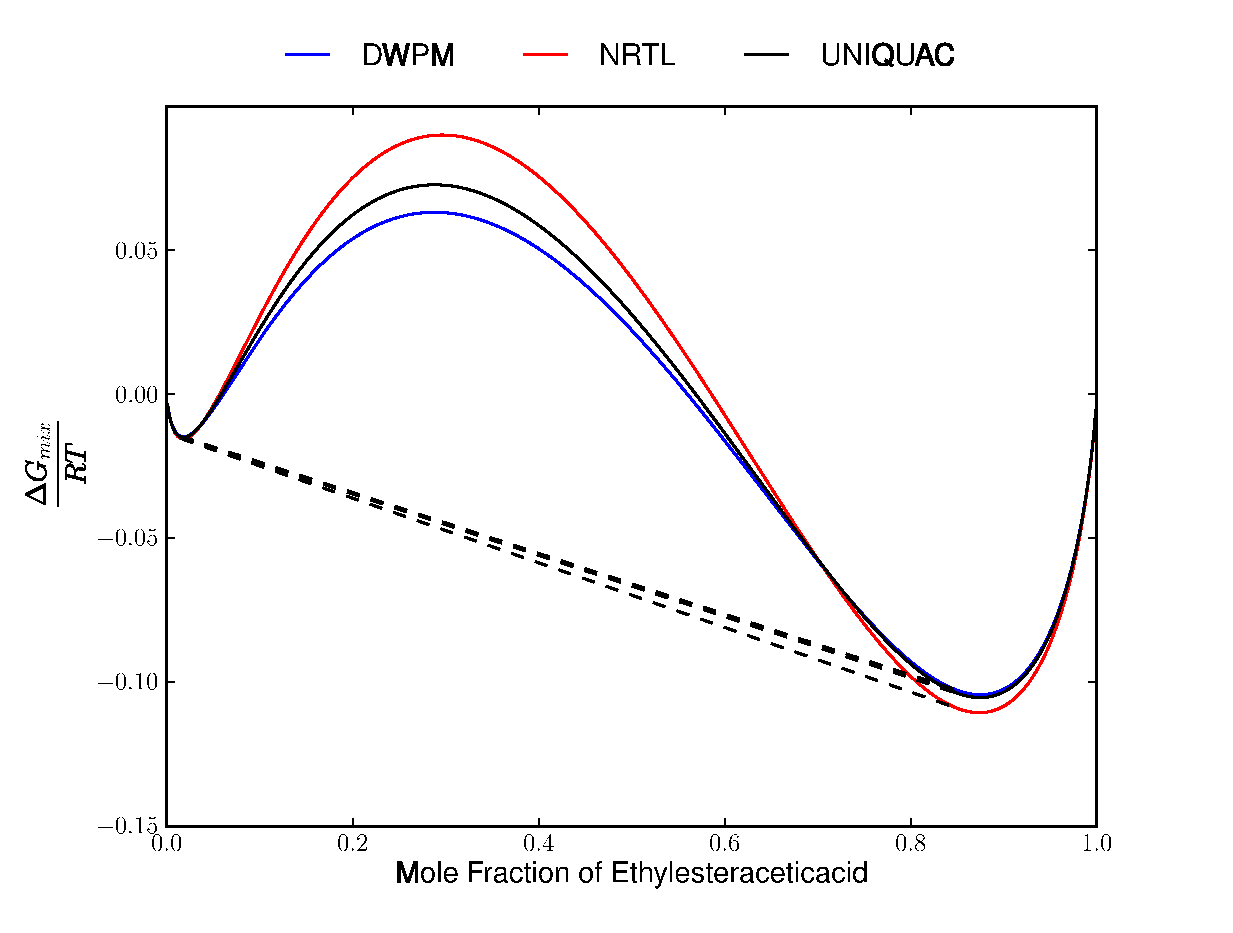
\includegraphics[width = \textwidth]{Results_Parts/BinaryParams/ethylesteraceticacid-water/AllModelsGibbsPlots/T_303.0.eps}
	\caption{303.0~$\mathrm{K}$}
\end{subfigure}%
~%
\begin{subfigure}[h]{0.5\textwidth}
	\centering
	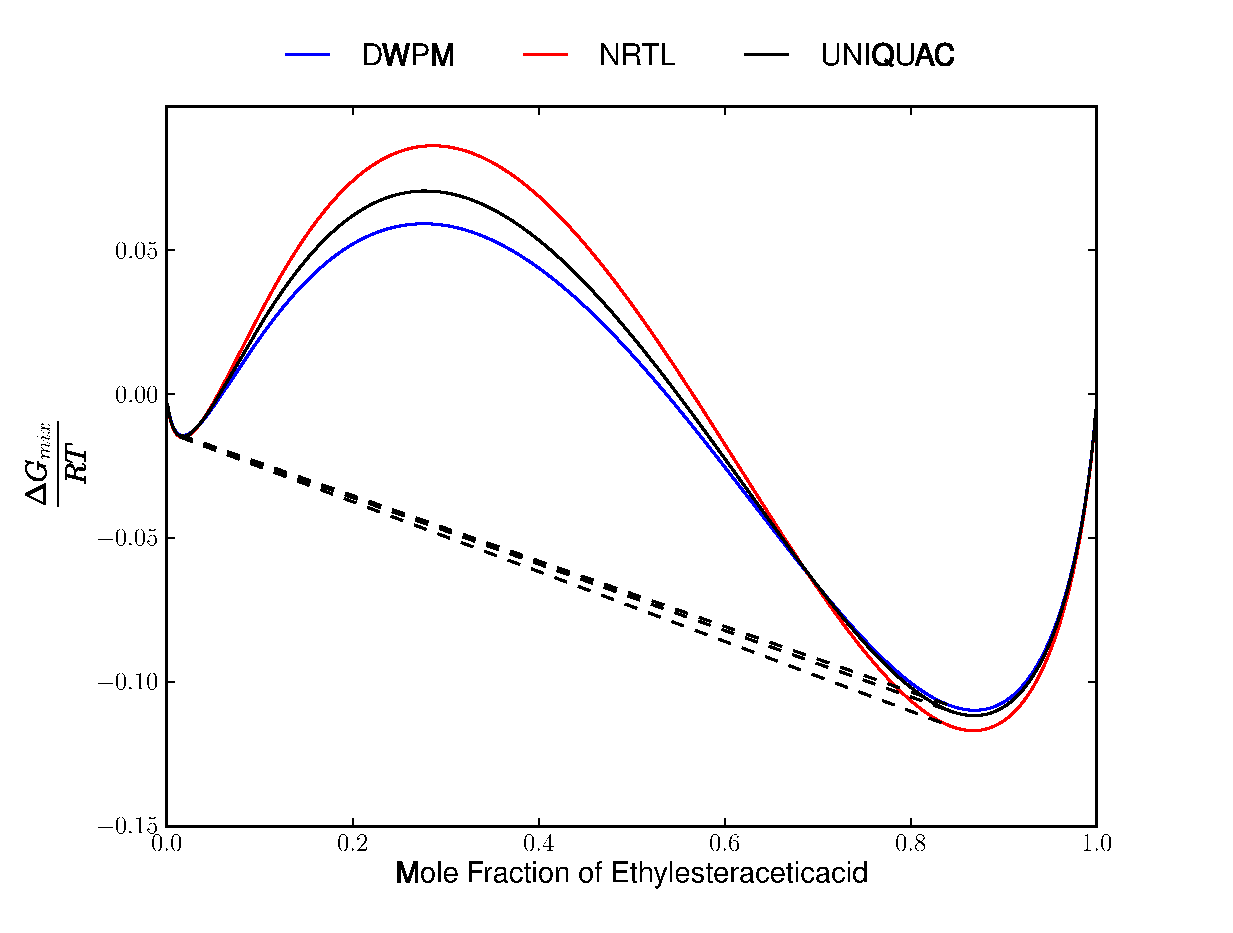
\includegraphics[width = \textwidth]{Results_Parts/BinaryParams/ethylesteraceticacid-water/AllModelsGibbsPlots/T_308.0.eps}
	\caption{308.0~$\mathrm{K}$}
\end{subfigure}%
\caption[]{Calculated liquid-liquid equilibrium for Ethyl Ester Acetic Acid and Water}
\end{figure}
\vspace*{\fill}
\clearpage
\begin{figure}[hpt]
\ContinuedFloat 
\begin{subfigure}[h]{0.5\textwidth}
	\centering
	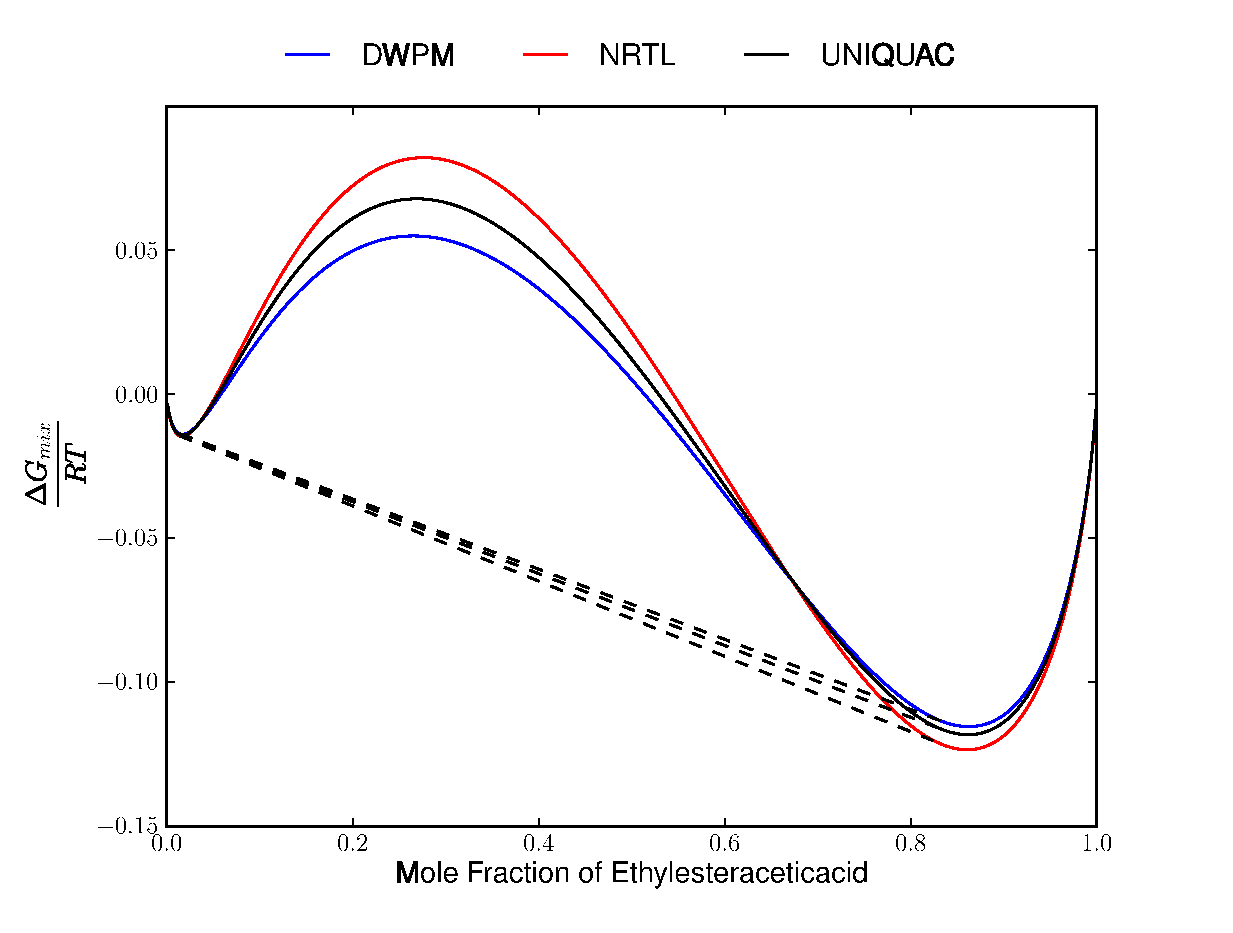
\includegraphics[width = \textwidth]{Results_Parts/BinaryParams/ethylesteraceticacid-water/AllModelsGibbsPlots/T_313.0.eps}
	\caption{313.0~$\mathrm{K}$}
\end{subfigure}%
\caption[]{Calculated liquid-liquid equilibrium for Ethyl Ester Acetic Acid and Water}
\end{figure}
\clearpage
%%----------------------------------------------------------------------------------------------------------------------------------------------%%

\subsection{Methanol and Heptane}
\vspace*{\fill}
\begin{figure}[hp]
\begin{subfigure}[h]{0.5\textwidth}
\centering
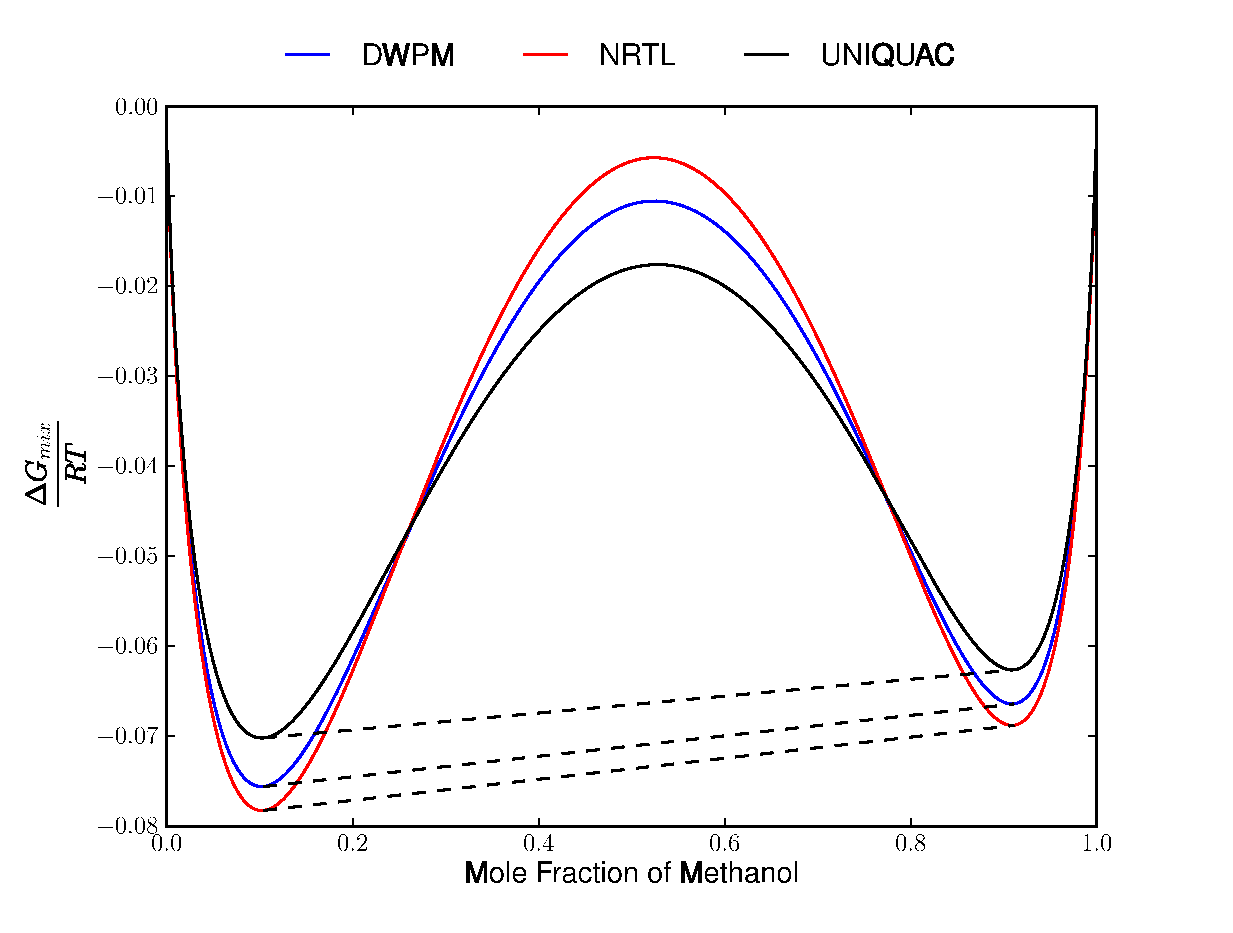
\includegraphics[width = \textwidth]{Results_Parts/BinaryParams/methanol-heptane/AllModelsGibbsPlots/T_291.eps}
\caption{291.0~$\mathrm{K}$} \label{methanol-heptane291}
\end{subfigure}%
~%
\begin{subfigure}[h]{0.5\textwidth}
\centering
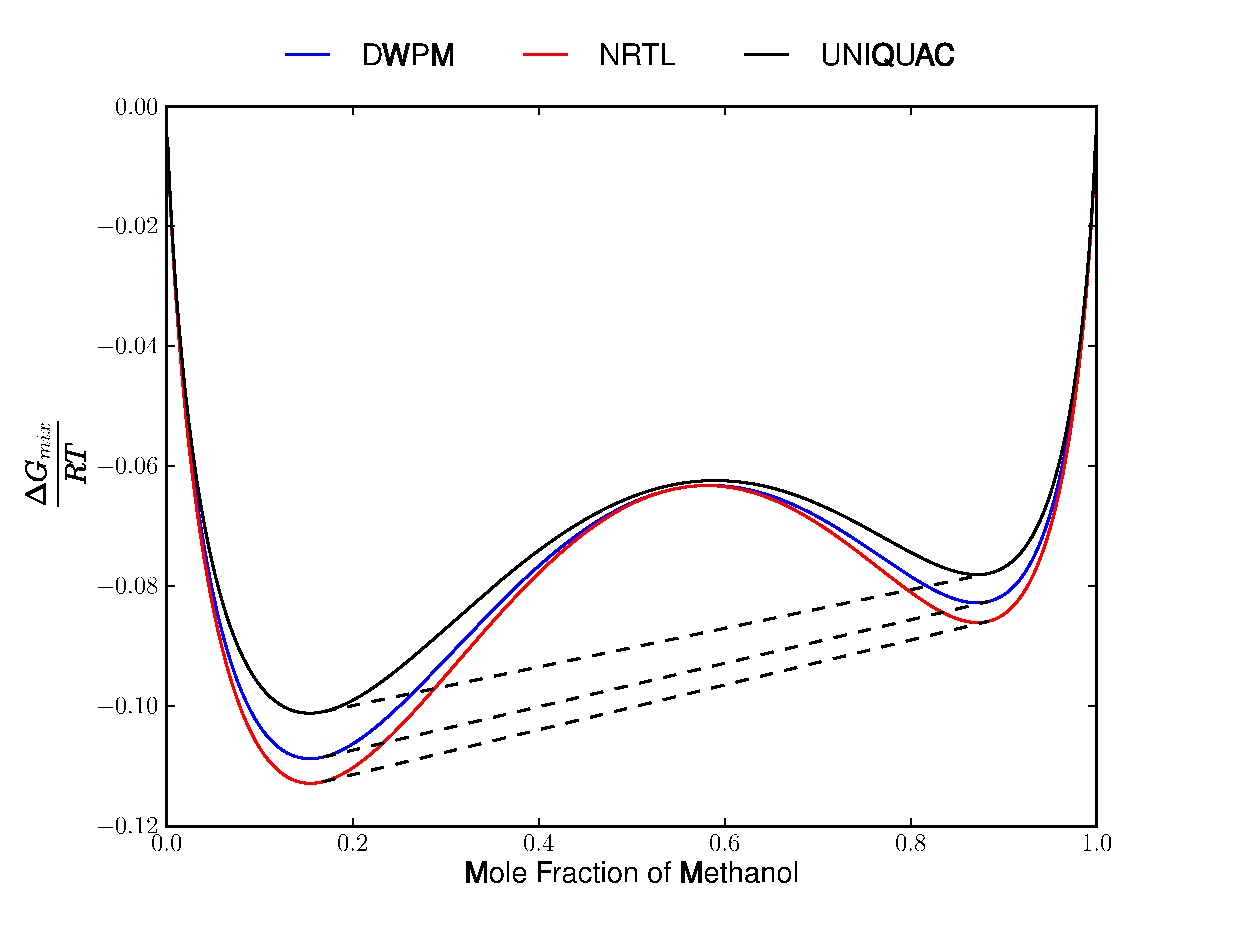
\includegraphics[width = \textwidth]{Results_Parts/BinaryParams/methanol-heptane/AllModelsGibbsPlots/T_303.eps}
\caption{303.0~$\mathrm{K}$} 
\end{subfigure}%
\\%
\begin{subfigure}[h]{0.5\textwidth}
\centering
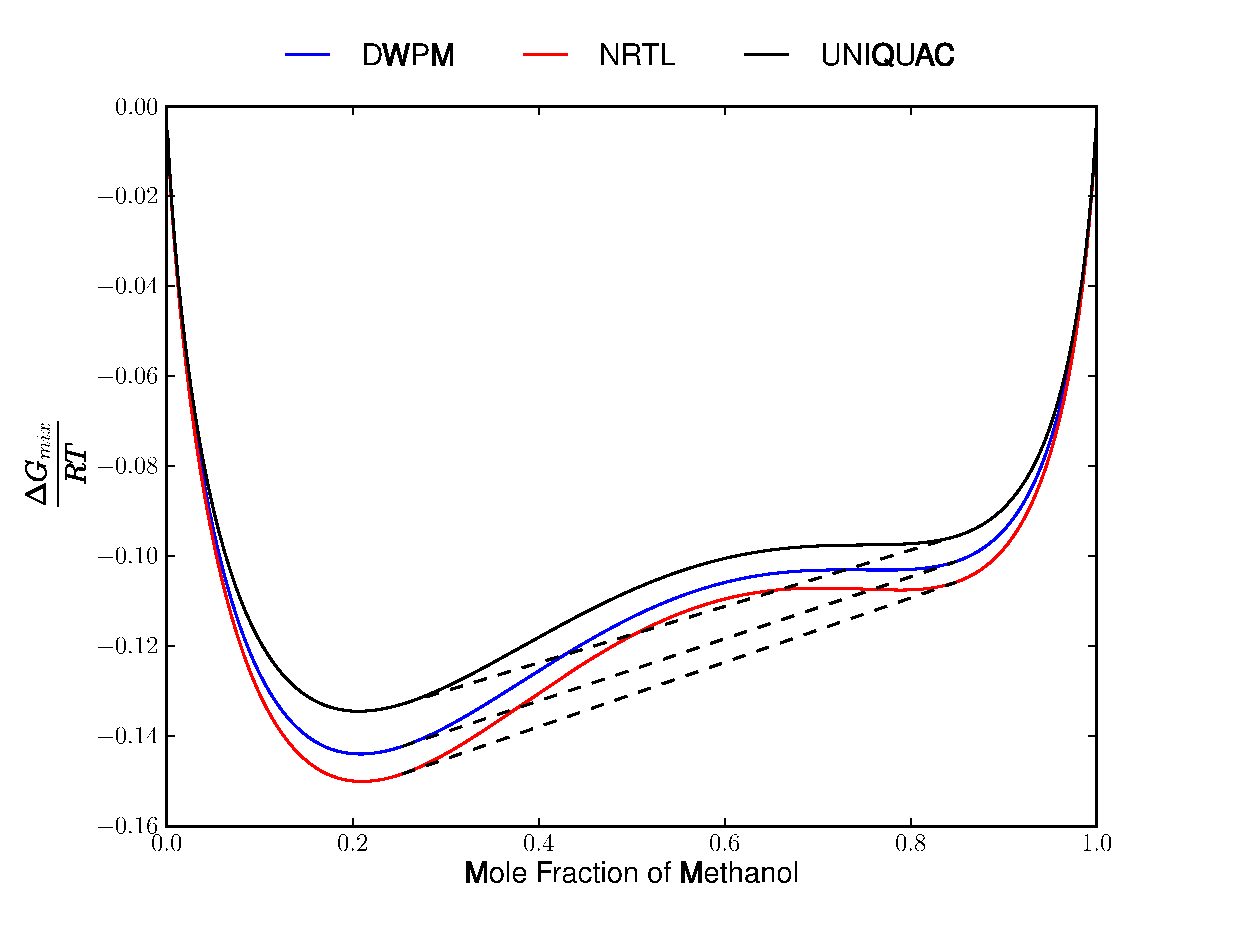
\includegraphics[width = \textwidth]{Results_Parts/BinaryParams/methanol-heptane/AllModelsGibbsPlots/T_313.eps}
\caption{313.0~$\mathrm{K}$} 
\end{subfigure}%
~%
\begin{subfigure}[h]{0.5\textwidth}
\centering
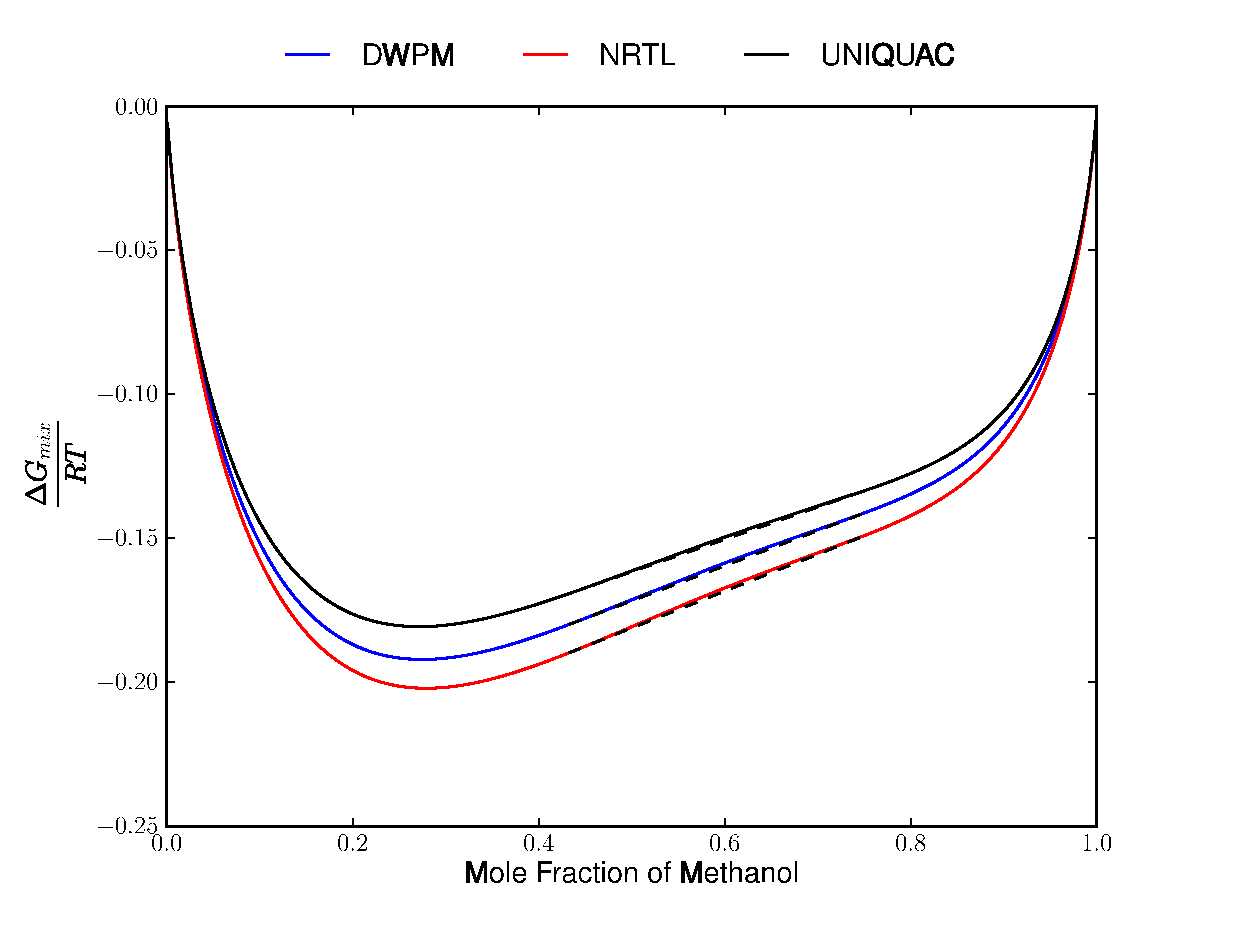
\includegraphics[width = \textwidth]{Results_Parts/BinaryParams/methanol-heptane/AllModelsGibbsPlots/T_323.eps}
\caption{323.0~$\mathrm{K}$} \label{methanol-heptane323}
\end{subfigure}%
\caption{Calculated liquid-liquid equilibrium for Methanol and Heptane}
\end{figure}
\vspace*{\fill}
\clearpage

%%-----------------------------------------------------------------------------------------------------------------------------------------------%%

\subsection{Methanol and Hexane}
\vspace*{\fill}
\begin{figure}[hp]
\begin{subfigure}[h]{0.5\textwidth}
\centering
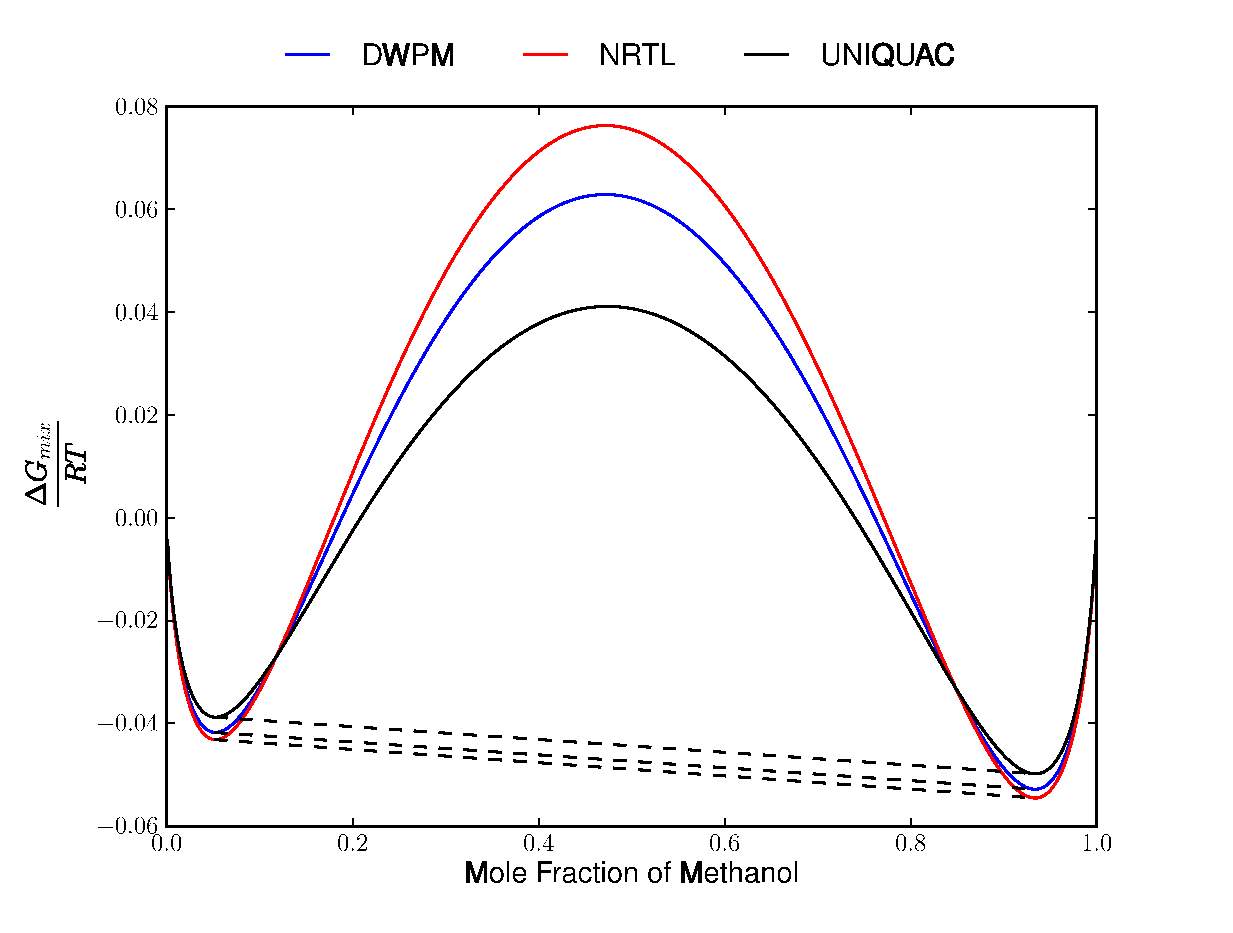
\includegraphics[width = \textwidth]{Results_Parts/BinaryParams/methanol-hexane/AllModelsGibbsPlots/T_255.2.eps}
\caption{255.2~$\mathrm{K}$} \label{methanol-hexane255}
\end{subfigure}%
~%
\begin{subfigure}[h]{0.5\textwidth}
\centering
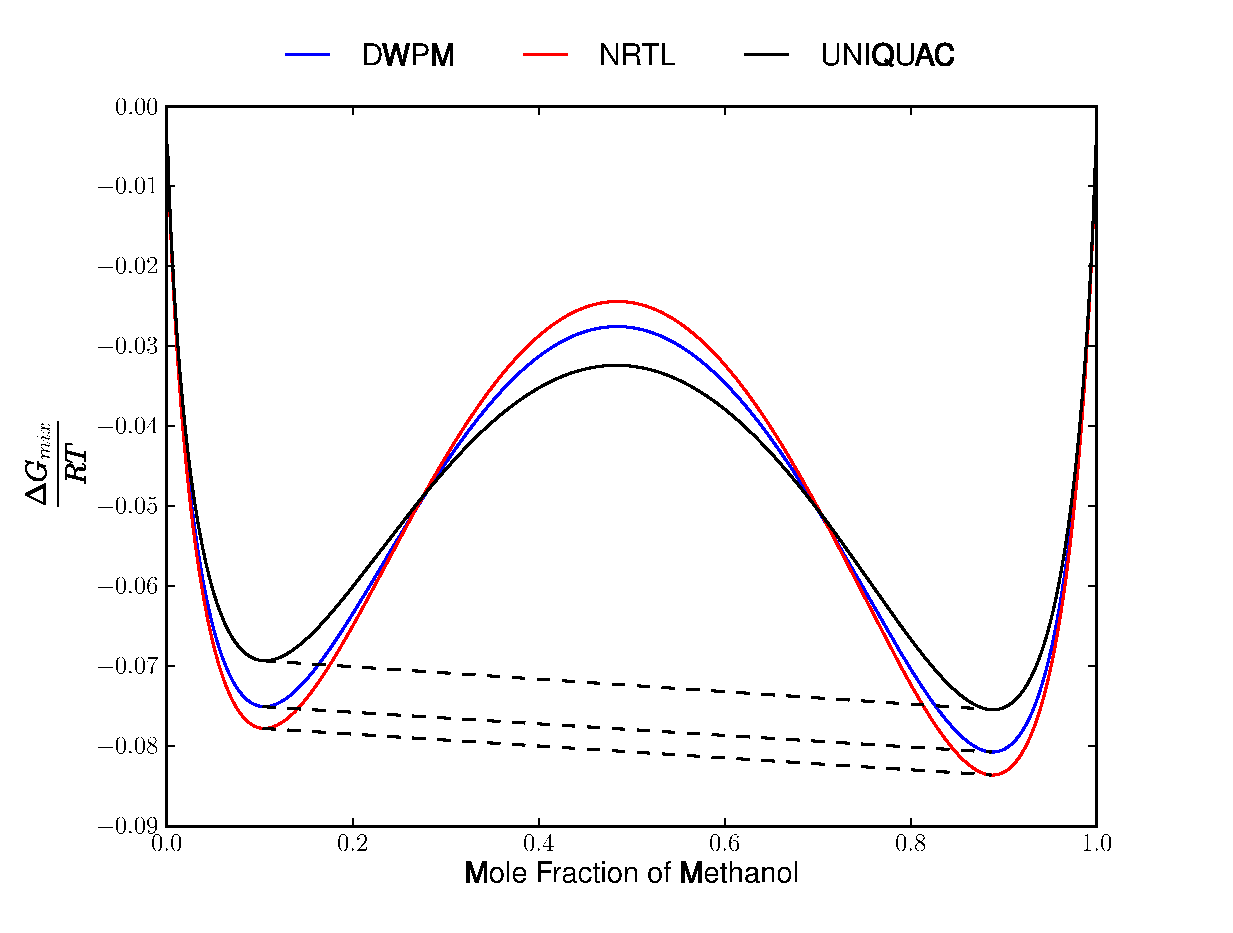
\includegraphics[width = \textwidth]{Results_Parts/BinaryParams/methanol-hexane/AllModelsGibbsPlots/T_278.0.eps}
\caption{278.0~$\mathrm{K}$} 
\end{subfigure}%
\\%
\begin{subfigure}[h]{0.5\textwidth}
\centering
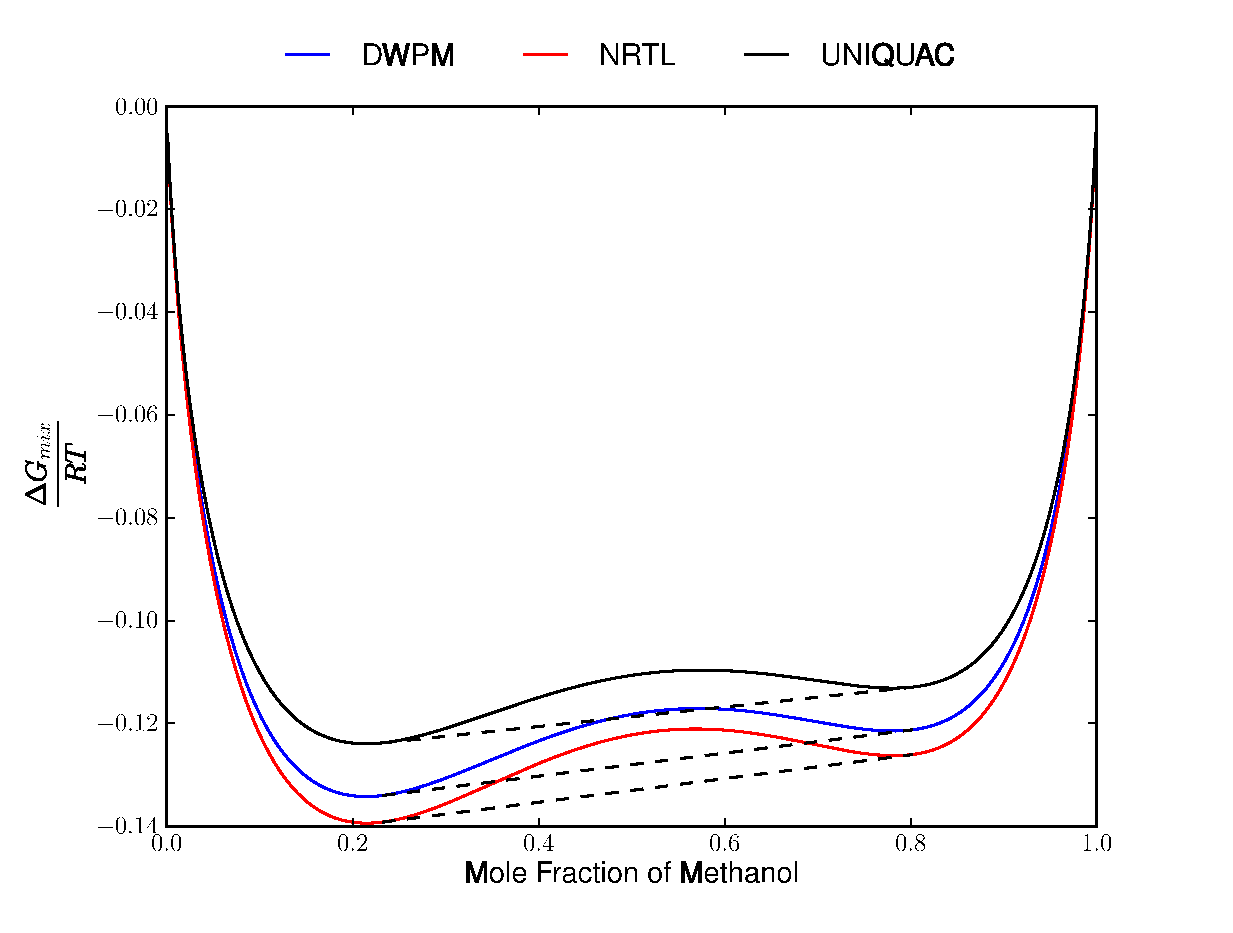
\includegraphics[width = \textwidth]{Results_Parts/BinaryParams/methanol-hexane/AllModelsGibbsPlots/T_298.0.eps}
\caption{298.0~$\mathrm{K}$} \label{methanol-hexane298}
\end{subfigure}%
\caption{Calculated liquid-liquid equilibrium for Methanol and Hexane}
\end{figure}
\vspace*{\fill}
\clearpage
	%\section{Gibbs Energy Surfaces of Ternary Mixtures}\label{AppendixGibbsPlotsTernaries}
	%	This section depicts the Gibbs energy surfaces predicted using the model parameters calculated from ternary liquid-liquid equilibrium data. The two experimental tie-lines, used for the pseudo-analytical method of parameter estimation, are indicated as solid black lines. In the figures that follow, regions where the Hessian matrix of the Gibbs energy function is not positive definite, i.~e. where the ternary mixture is unstable, are projected below the  Gibbs energy surface and indicated in red.\\

%%------------------------------- Cyclohexane, Benzene and Nitro-Methane-------------------------------------------%
\subsection{Cyclohexane, Benzene and Nitro-Methane}

\begin{figure}[hp]
 \vspace{40pt}
\centering
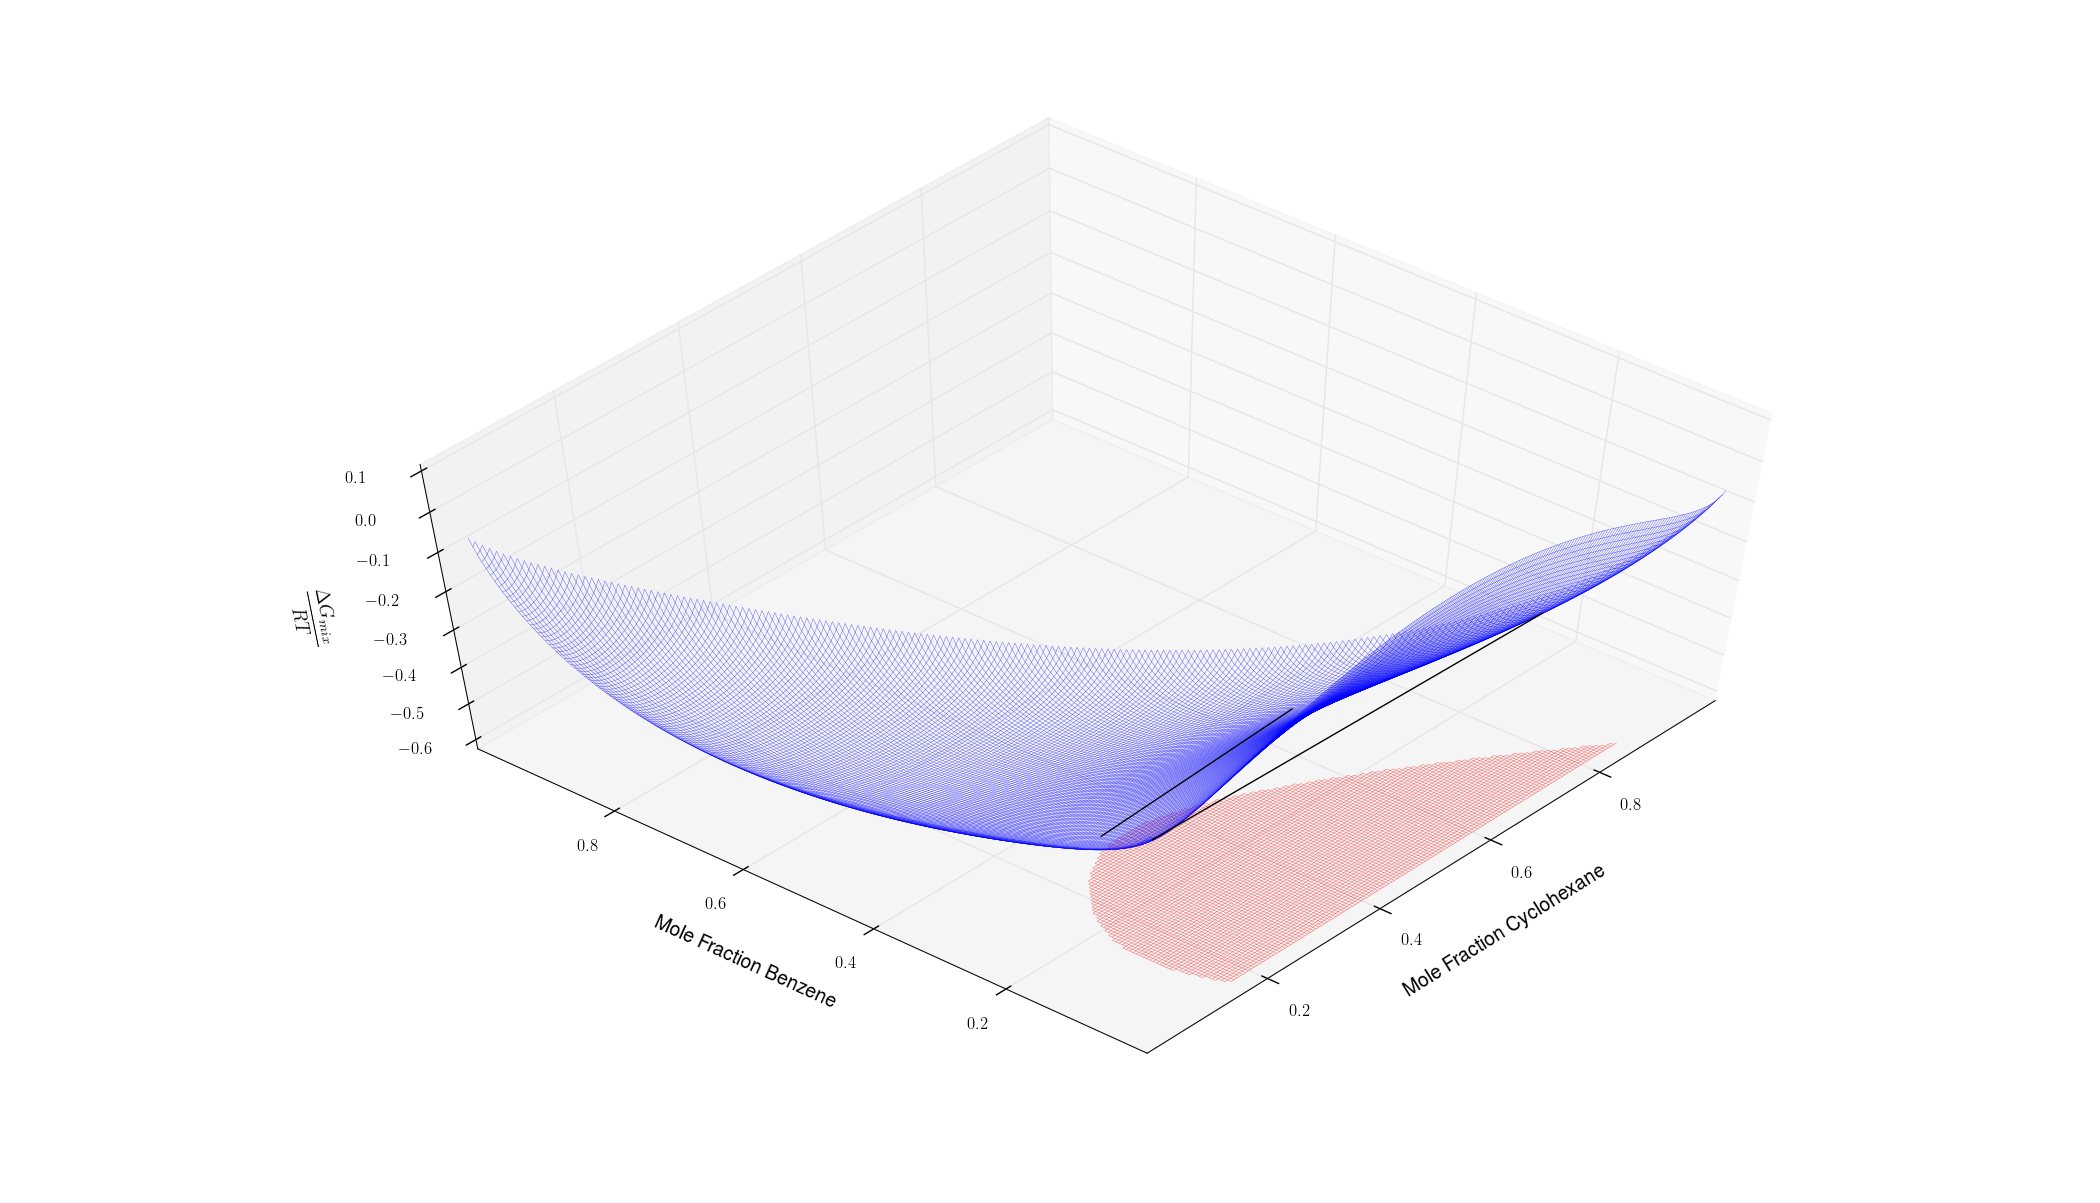
\includegraphics[width = \textwidth, bb=100 100 1600 700]{Results_Parts/TernaryParams/cyclohexane-benzene-methanenitro/DWPM/rotation1.png}
\caption{Predicted Gibbs energy surface for Cyclohexane, Benzene and Nitro-Methane at $298.15~\mathrm{K}$}
\end{figure}	

\begin{figure}[hp]
\vspace{40pt}
\ContinuedFloat
\centering
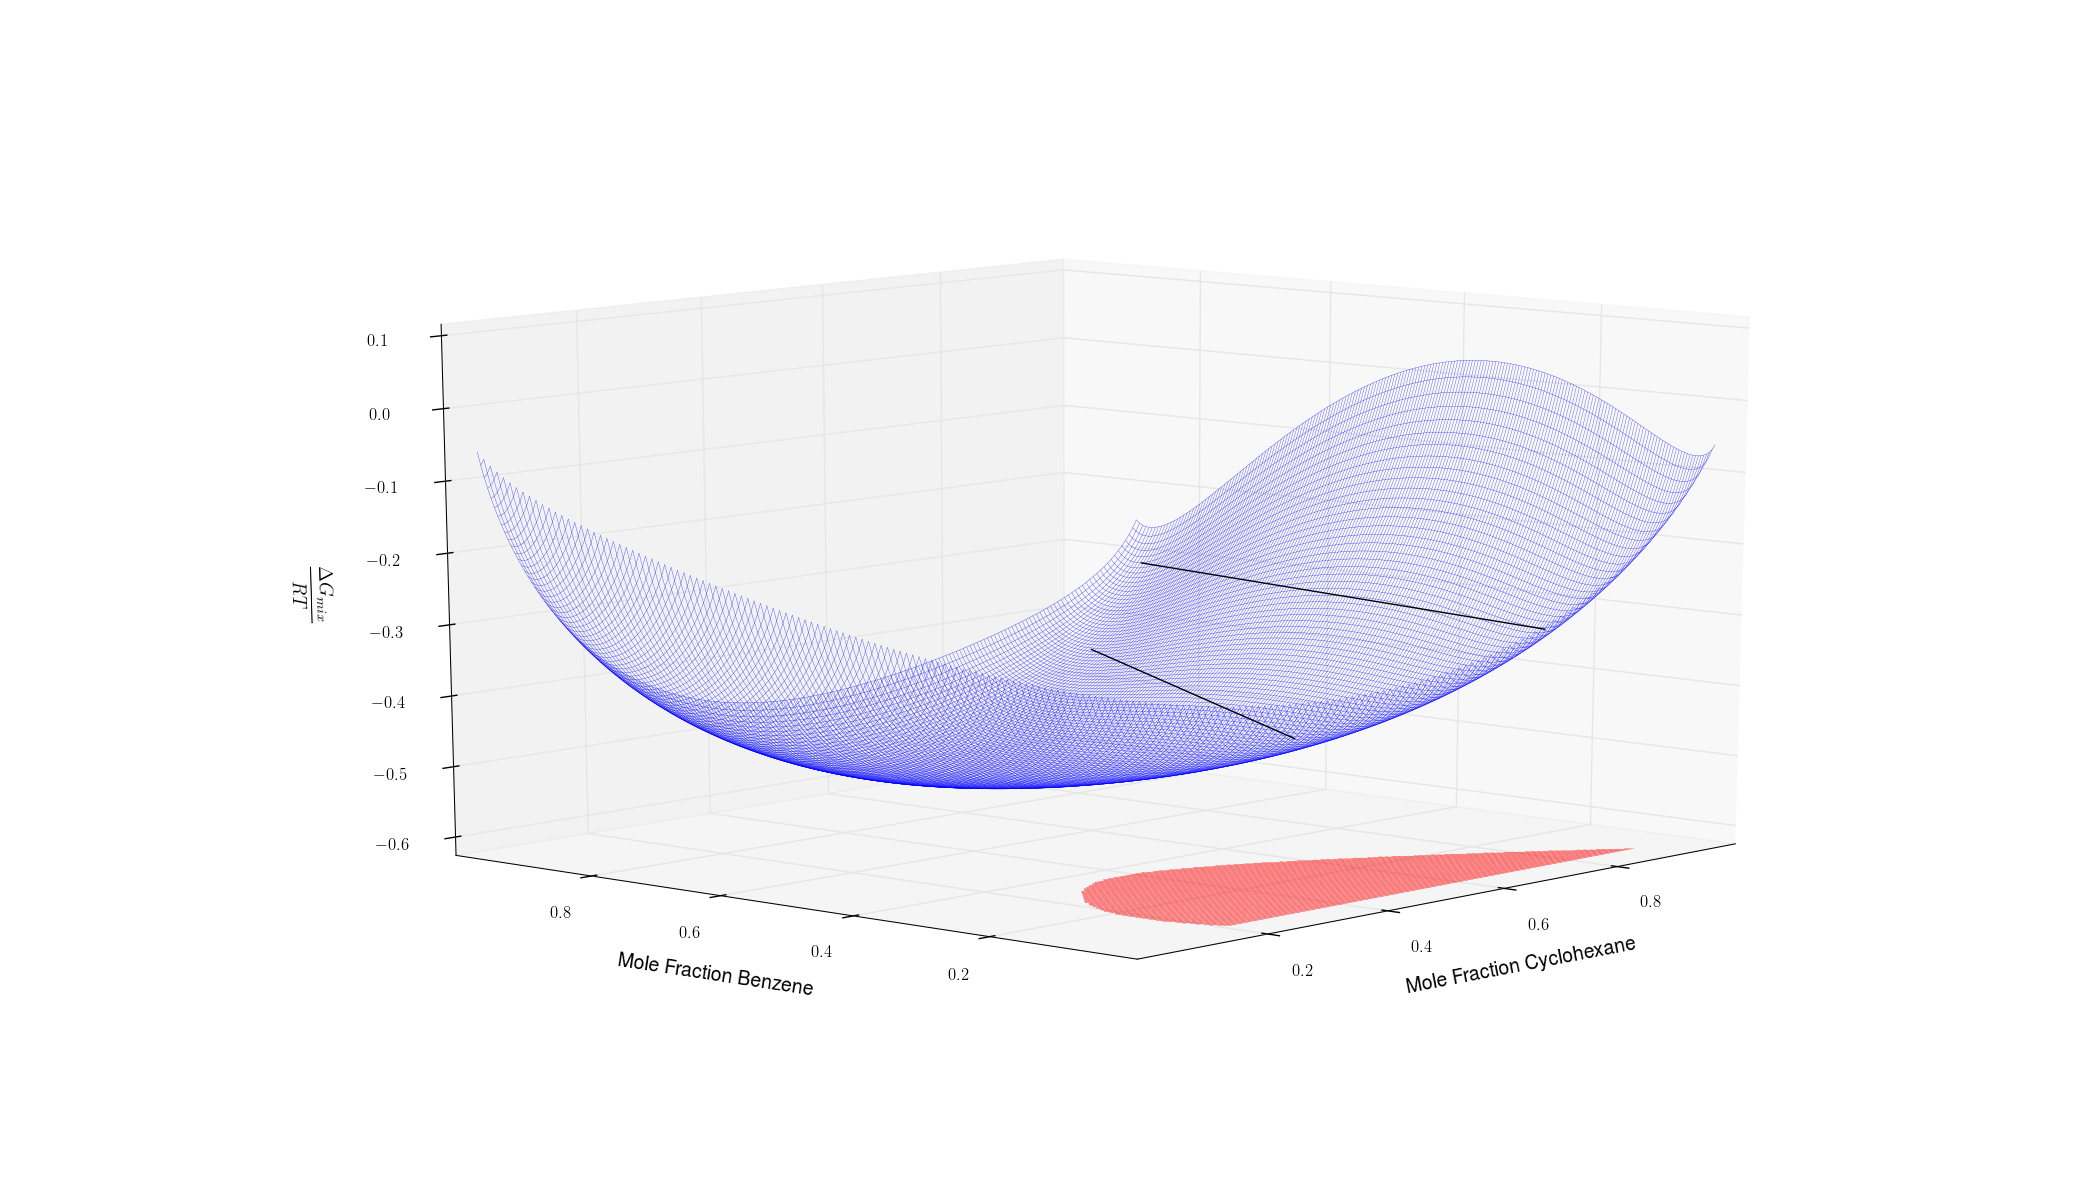
\includegraphics[width = \textwidth, bb=100 100 1600 700]{Results_Parts/TernaryParams/cyclohexane-benzene-methanenitro/DWPM/rotation2.png}
\caption[]{(Continued) Rotated View 1}
\end{figure}

\begin{figure}[hp]
\vspace{40pt}
\ContinuedFloat
\centering
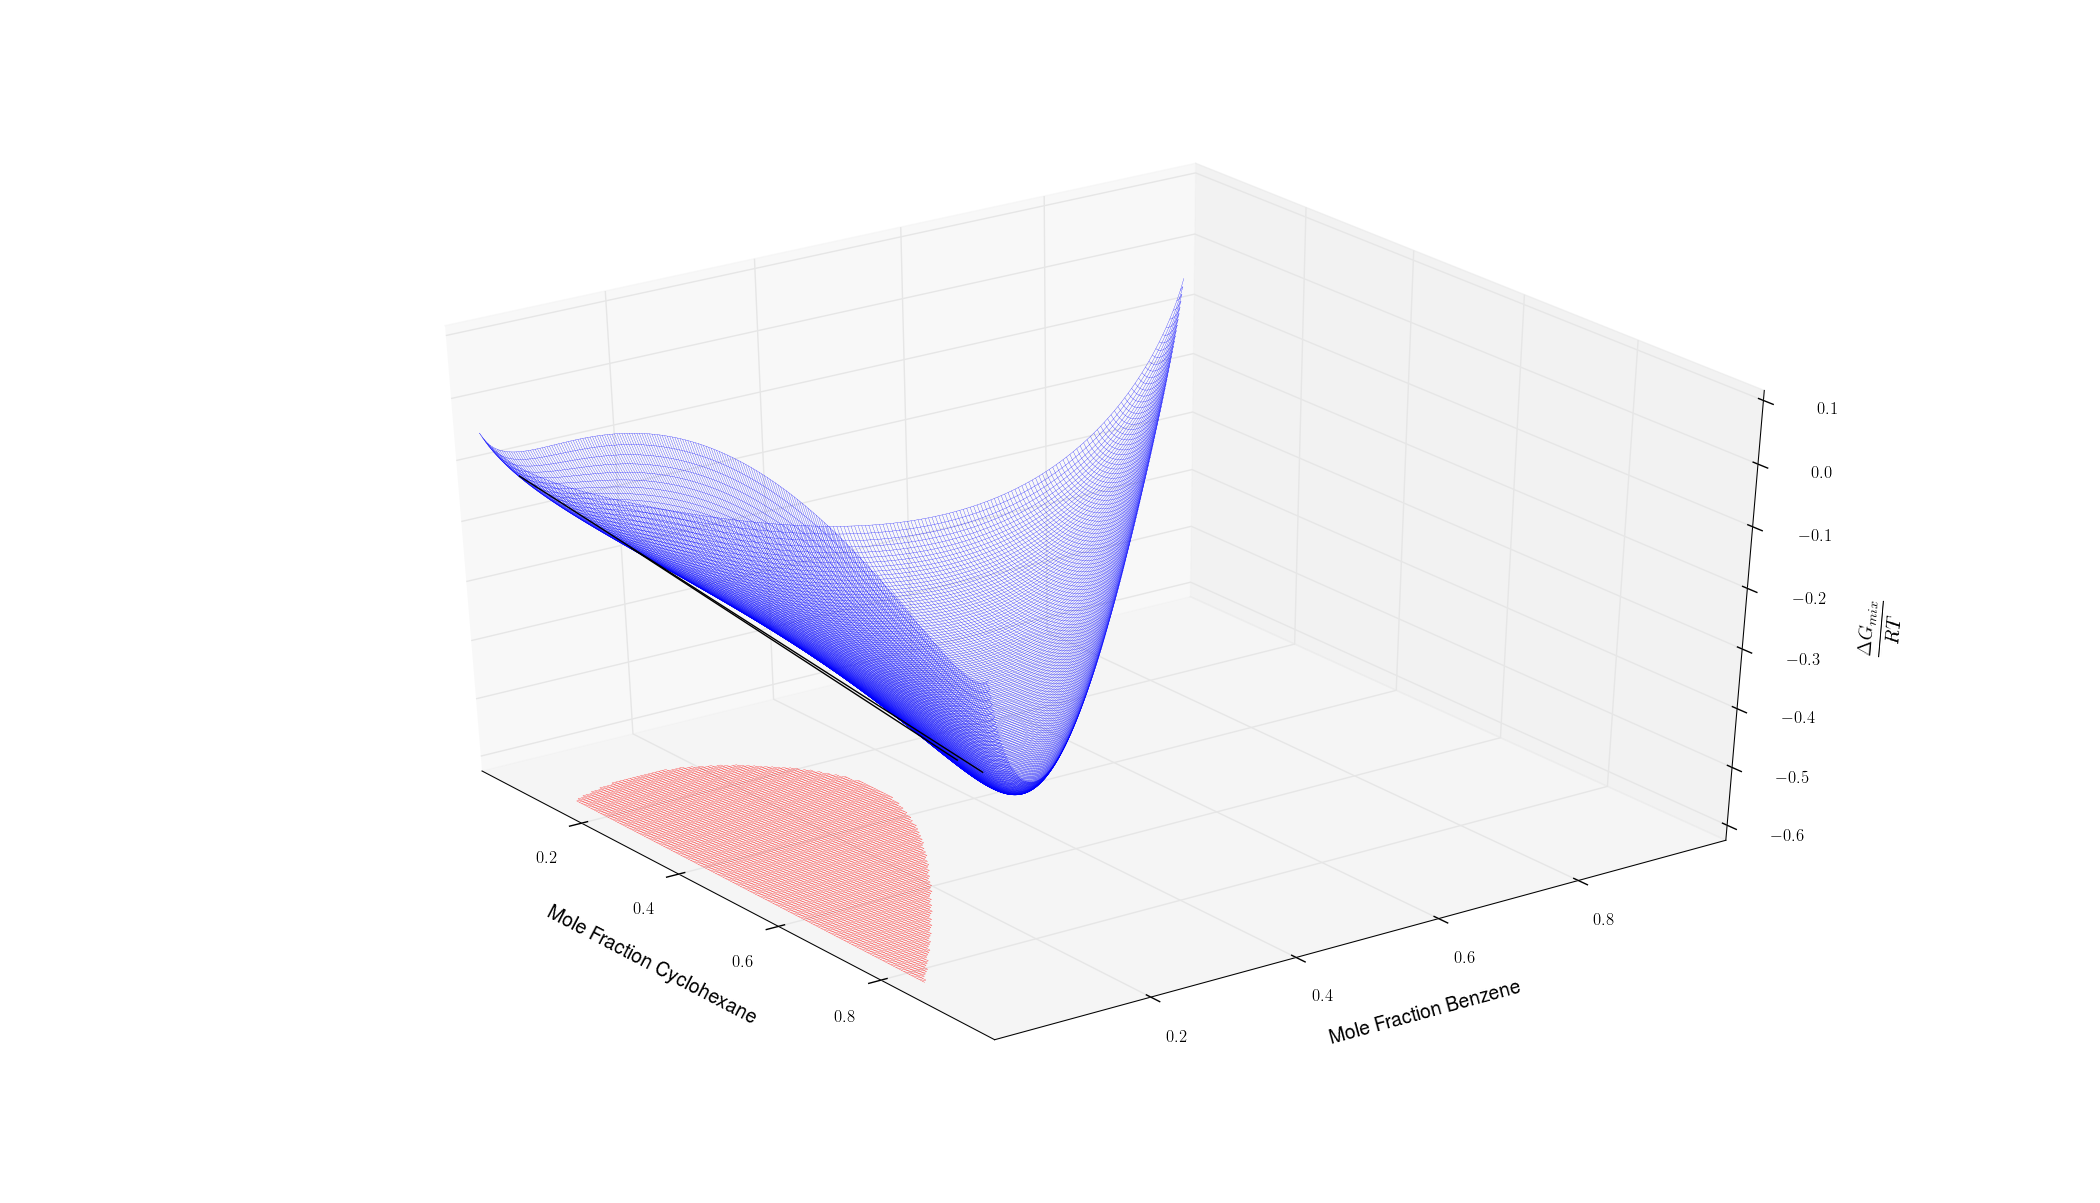
\includegraphics[width = \textwidth, bb=100 100 1600 700]{Results_Parts/TernaryParams/cyclohexane-benzene-methanenitro/DWPM/rotation5.png}
\caption[]{(Continued) Rotated View 2}
\end{figure}

\begin{figure}[hp]
\vspace{40pt}
\ContinuedFloat
\centering
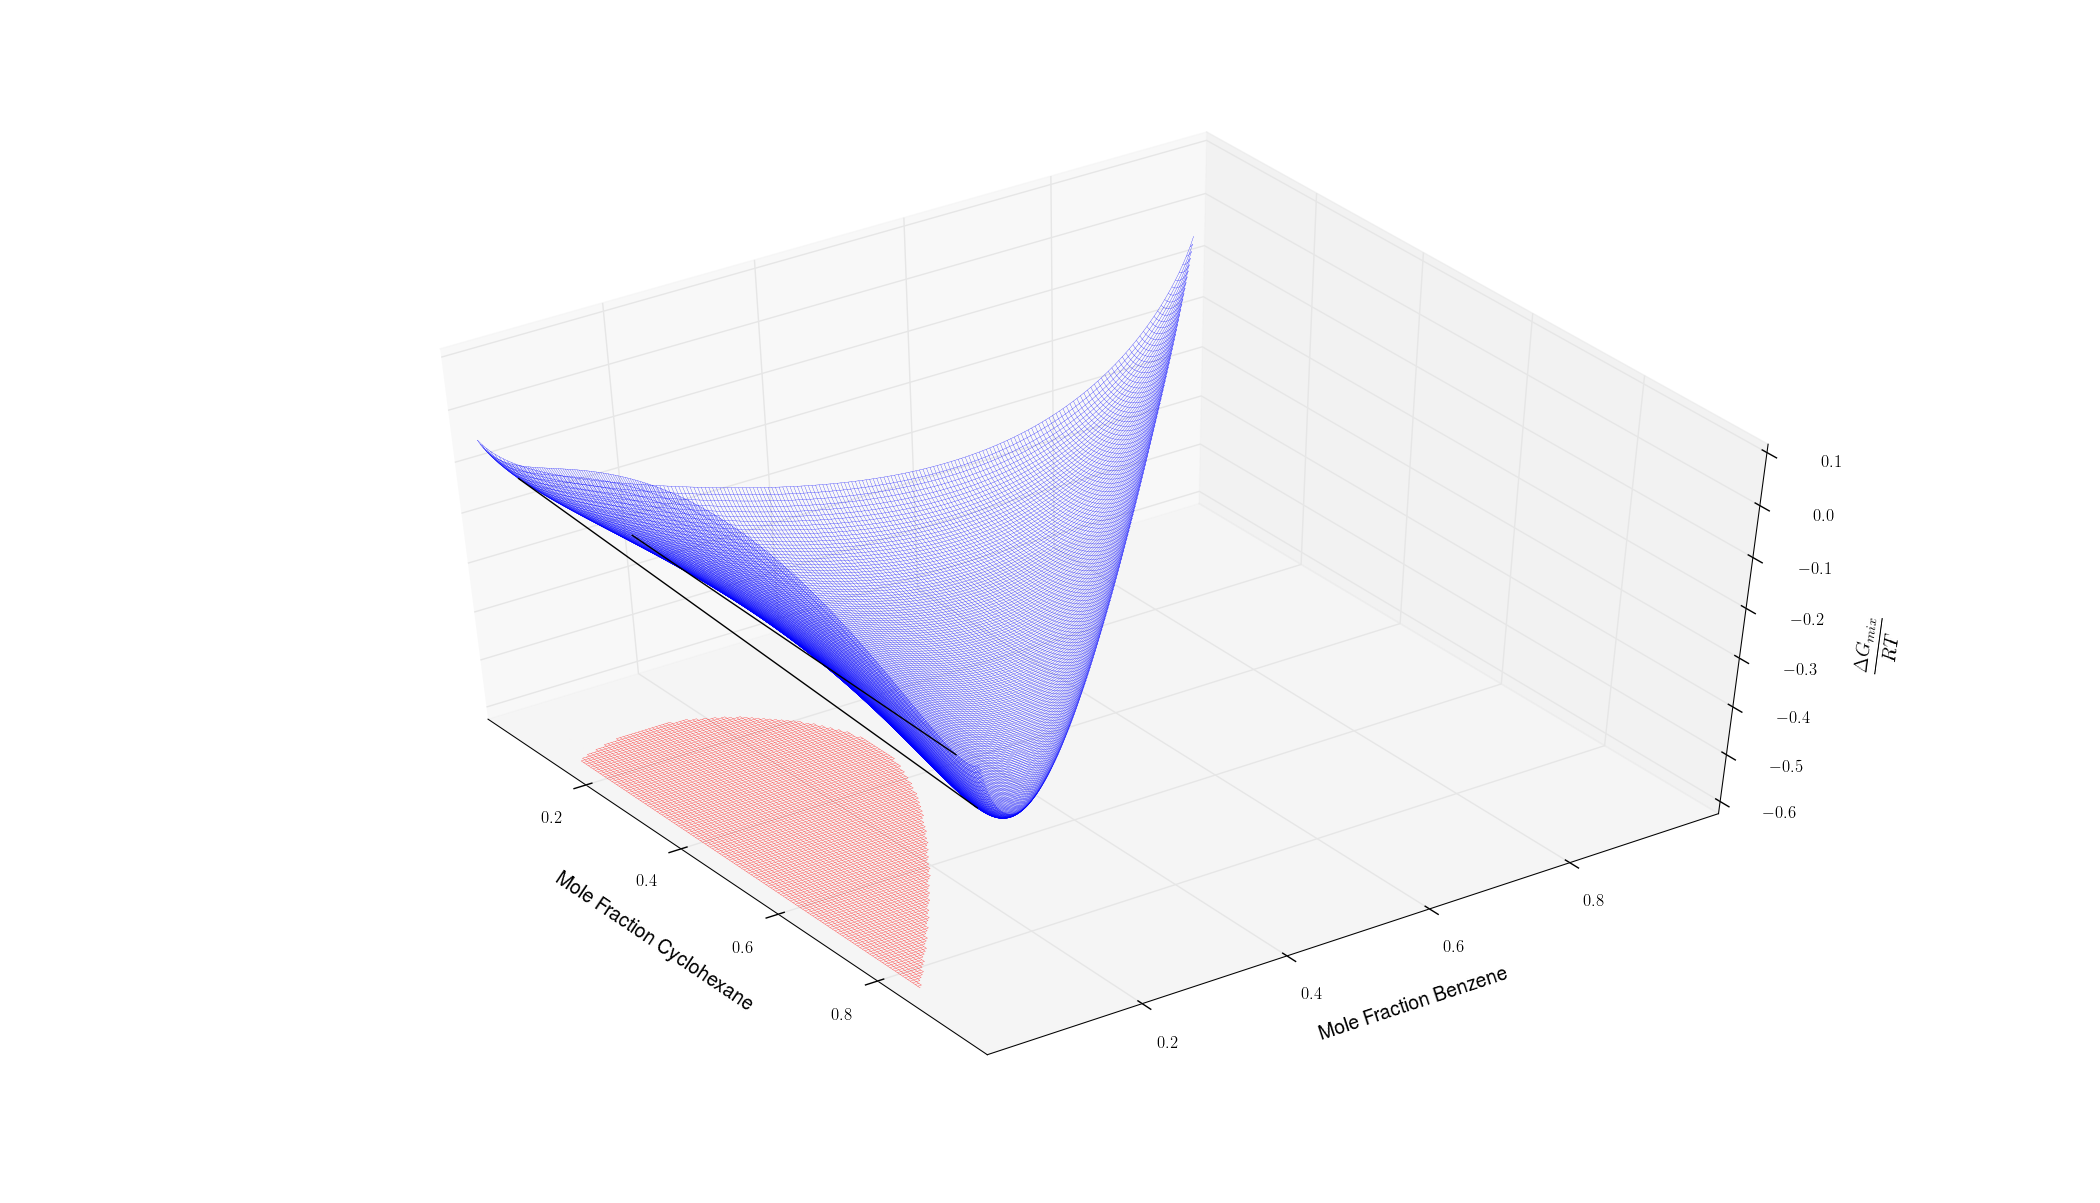
\includegraphics[width = \textwidth, bb=100 100 1600 700]{Results_Parts/TernaryParams/cyclohexane-benzene-methanenitro/DWPM/rotation6.png}
\caption[]{(Continued) Rotated View 3}
\end{figure}
\clearpage

%%------------------------------- Heptane, Hexane and Methanol-------------------------------------------%
\subsection{Heptane, Hexane and Methanol}

\begin{figure}[hp]
 \vspace{40pt}
\centering
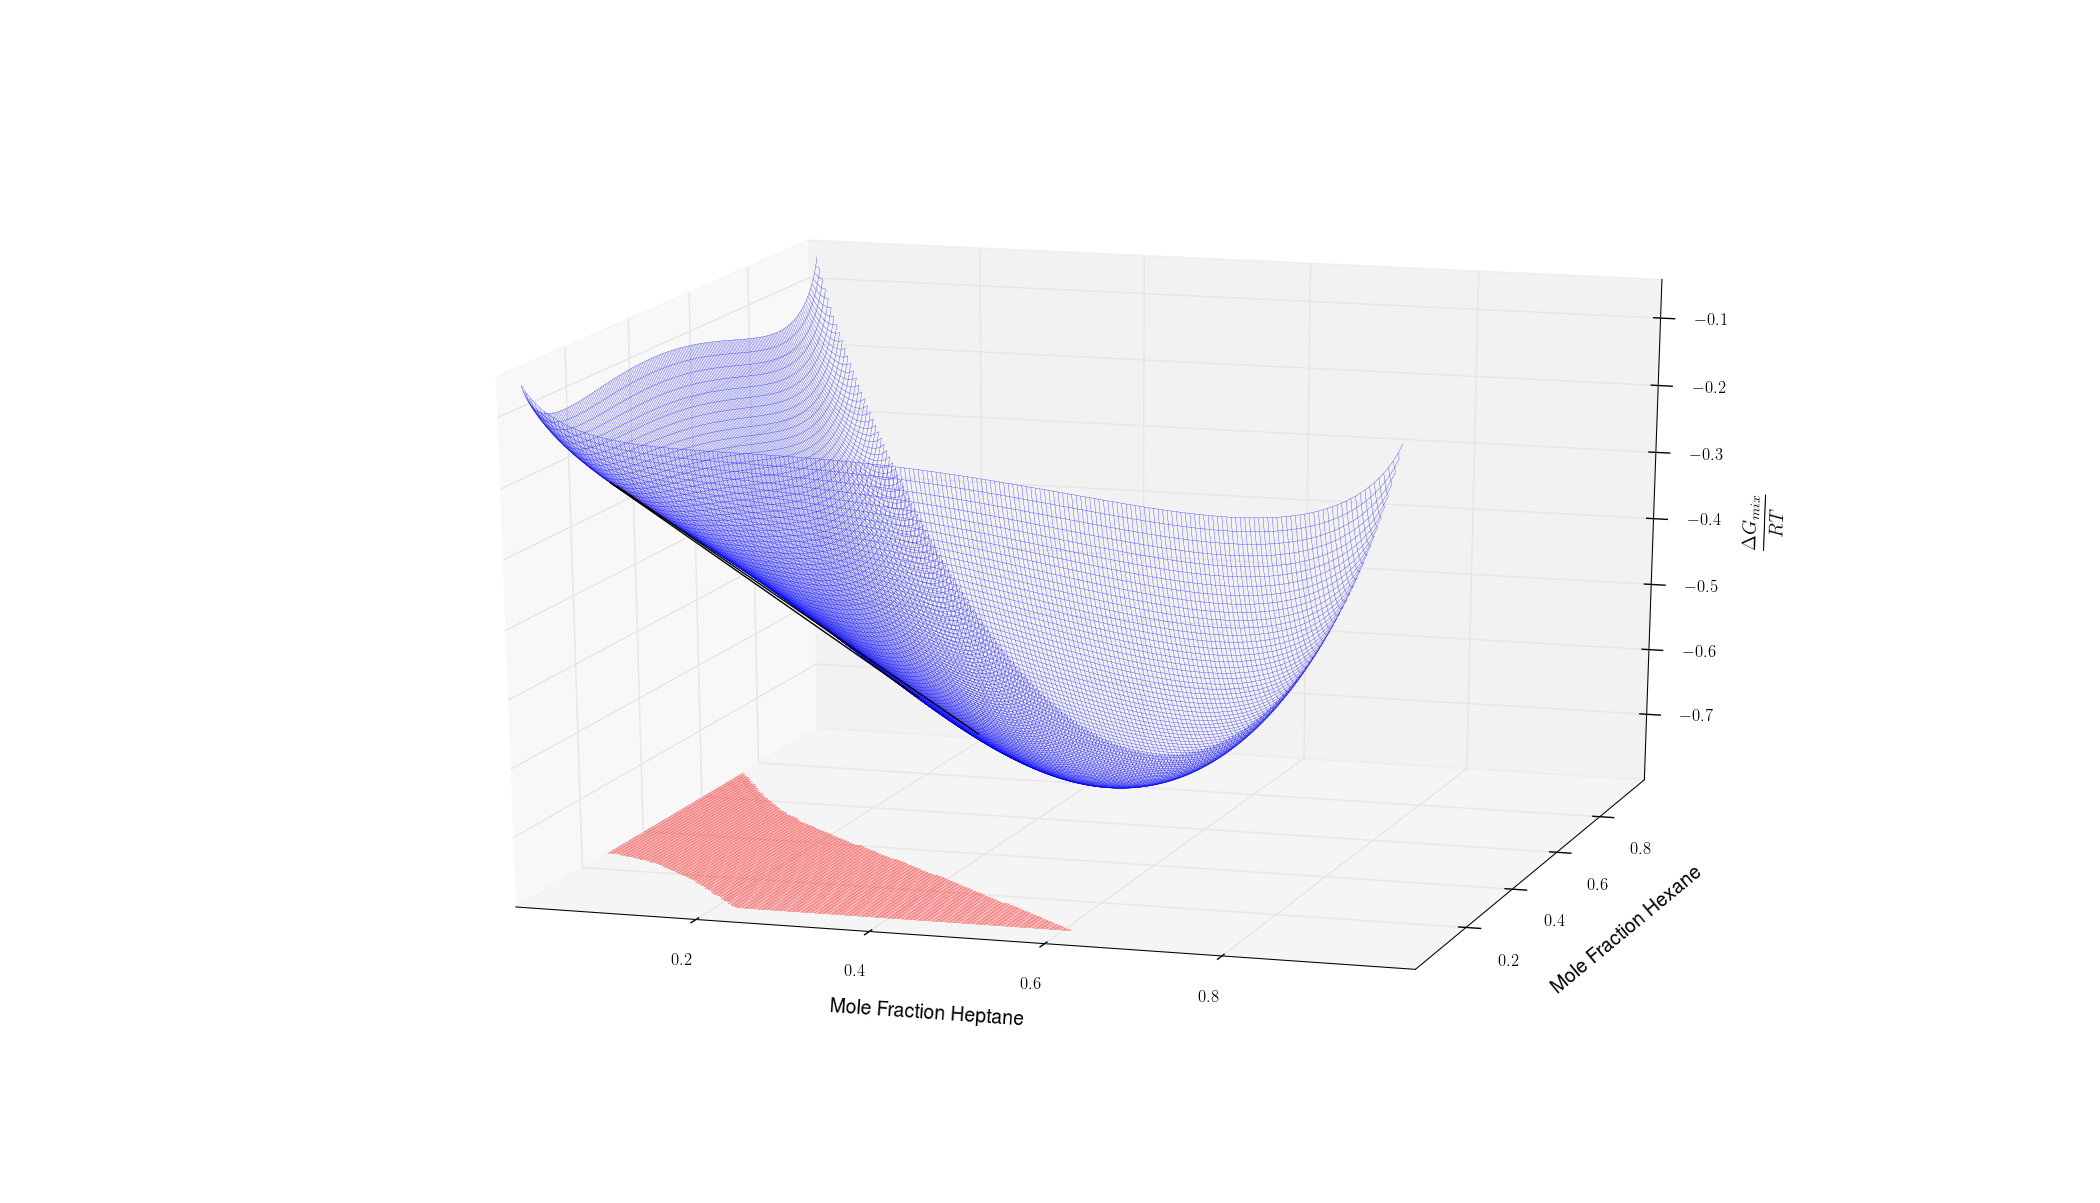
\includegraphics[width = \textwidth, bb=100 100 1600 700]{Results_Parts/TernaryParams/heptane-hexane-methanol/DWPMTieline3and4/rotation4.png}
\caption{Predicted Gibbs energy surface for Heptane, Hexane and Methanol at $305.95~\mathrm{K}$, using parameters calculated from experimental tie-lines 3 and 4.}
\end{figure}	

\begin{figure}[hp]
\vspace{40pt}
\ContinuedFloat
\centering
\includegraphics[width = \textwidth, bb=100 100 1600 700]{Results_Parts/TernaryParams/heptane-hexane-methanol/DWPMTieline3and4/rotation3.png}
\caption[]{(Continued) Rotated View 1}
\end{figure}

\begin{figure}[hp]
\vspace{40pt}
\ContinuedFloat
\centering
\includegraphics[width = \textwidth, bb=100 100 1600 700]{Results_Parts/TernaryParams/heptane-hexane-methanol/DWPMTieline3and4/rotation6.png}
\caption[]{(Continued) Rotated View 2}
\end{figure}

\begin{figure}[hp]
\vspace{40pt}
\ContinuedFloat
\centering
\includegraphics[width = \textwidth, bb=100 100 1600 700]{Results_Parts/TernaryParams/heptane-hexane-methanol/DWPMTieline3and4/rotation8.png}
\caption[]{(Continued) Rotated View 3}
\end{figure}

\clearpage

\begin{figure}[hp]
 \vspace{40pt}
\centering
\includegraphics[width = \textwidth, bb=100 100 1600 700]{Results_Parts/TernaryParams/heptane-hexane-methanol/DWPMTieline3and-2/rotation6.png}
\caption{Predicted Gibbs energy surface for Heptane, Hexane and Methanol at $305.95~\mathrm{K}$, using parameters calculated from experimental tie-lines 3 and second to last.}
\end{figure}	

\begin{figure}[hp]
\vspace{40pt}
\ContinuedFloat
\centering
\includegraphics[width = \textwidth, bb=100 100 1600 700]{Results_Parts/TernaryParams/heptane-hexane-methanol/DWPMTieline3and-2/rotation2.png}
\caption[]{(Continued) Rotated View 1}
\end{figure}

\begin{figure}[hp]
\vspace{40pt}
\ContinuedFloat
\centering
\includegraphics[width = \textwidth, bb=100 100 1600 700]{Results_Parts/TernaryParams/heptane-hexane-methanol/DWPMTieline3and-2/rotation4.png}
\caption[]{(Continued) Rotated View 2}
\end{figure}

\clearpage
%%------------------------------- 1-Hexanol, Nitro-Methane and Water-------------------------------------------%
\subsection{1-Hexanol, Nitro-Methane and Water}

\begin{figure}[hp]
\centering
\includegraphics[width = 0.6\textwidth, bb=100 0 500 400]{Results_Parts/TernaryParams/1-hexanol-methanenitro-water/DWPM/294.15/PredictedGibbsWireframe.png}
\caption{Predicted Gibbs energy surface for 1-Hexanol, Nitro-Methane and Water at $294.15~\mathrm{K}$.}
\end{figure}	


\begin{figure}[hp]
\centering
\includegraphics[width = 0.6\textwidth, bb=100 0 500 400]{Results_Parts/TernaryParams/1-hexanol-methanenitro-water/DWPM/296.15/PredictedGibbsWireframe.png}
\caption{Predicted Gibbs energy surface for 1-Hexanol, Nitro-Methane and Water at $296.15~\mathrm{K}$.}
\end{figure}


		
\end{document}